\documentclass[12pt, draftcls, onecolumn]{IEEEtran}

\usepackage{bm}
\usepackage{verbatim}
\usepackage{algorithm}
\usepackage{soul,xcolor}
\usepackage[T1]{fontenc}
\usepackage{algcompatible}
\usepackage[normalem]{ulem}
\usepackage{multirow,enumitem}
\usepackage{graphicx}

\usepackage{url}
\usepackage{bbm}
\usepackage{cite}
\usepackage{array}
\usepackage{ifthen}
\usepackage{xspace}
\usepackage{dsfont}
\usepackage{amsmath}
\usepackage{amssymb}
\usepackage{multicol}
\usepackage{amsfonts}
\usepackage{mathrsfs}
\usepackage{booktabs}
\usepackage{caption}
\usepackage{subcaption}
\usepackage{algpseudocode}

\usepackage{esint}
\usepackage{amsthm}
\usepackage{cancel}
\usepackage{siunitx}
\usepackage{setspace}
\usepackage{hyperref}
\usepackage{makecell}
\usepackage{footnote}

\captionsetup{font=small}
\captionsetup[sub]{font=footnotesize}

\renewcommand\qedsymbol{$\blacksquare$}

\renewcommand\theadalign{c}
\renewcommand\theadfont{\bfseries}
\renewcommand\cellgape{\Gape[2pt]}
\renewcommand\theadgape{\Gape[2pt]}

\theoremstyle{plain}
\newtheorem{lemma}{Lemma}
\newtheorem{theorem}{Theorem}

\theoremstyle{definition}
\newtheorem{defi}{Definition}
\newtheorem{corollary}{Corollary}

\theoremstyle{remark}
\newtheorem{remark}{Remark}
\newtheorem{nota}{Notation}

\newcommand{\tot}{\mathrm{tot}}
\newcommand{\numberthis}{\addtocounter{equation}{1}\tag{\theequation}}

\sisetup{detect-all,range-phrase=--,range-units=single}
\newcommand\mst[2][red]{\setbox0=\hbox{$#2$}\rlap{\raisebox{.45\ht0}{\textcolor{#1}{\rule{\wd0}{2pt}}}}#2}

\newcommand{\bk}[1]{\textcolor{blue}{[BK: #1]}}
\newcommand{\mb}[1]{\textcolor{blue}{[MB: #1]}}
\newcommand{\nm}[1]{\textcolor{magenta}{[NM: #1]}}

\newcommand{\sst}[1]{\st{#1}}
\newcommand{\prob}{\mathbb{P}}
\newcommand{\tfr}{T_{\mathrm{fr}}}
\newcommand{\vect}[1]{\mathbf{#1}}
\newcommand{\wtot}{W_{\mathrm{tot}}}
\newcommand{\add}[1]{\textcolor{red}{#1}}

\DeclareMathOperator{\Exp}{\mathbb{E}}
\DeclareMathOperator*{\argmax}{arg\,max}
\DeclareMathOperator*{\argmin}{arg\,min}

\newcommand{\tfrm}{T_{\mathrm{fr}}}
\newcommand{\beam}[1]{\mathcal B_{#1}}
\newcommand{\size}[1]{\left | #1 \right|}
\newcommand{\beambs}[1]{\mathcal B_{{\mathrm t},#1}}
\newcommand{\beamue}[1]{\mathcal B_{{\mathrm r},#1}}
\newcommand{\diag}[1]{\mathrm{diag}\left(#1 \right)}

\setlength{\textfloatsep}{1.5pt}

\title{MAESTRO-X: Distributed Orchestration of Rotary-Wing UAV Relay Swarms}
\author{Bharath Keshavamurthy\IEEEauthorrefmark{1}, Matthew A. Bliss\IEEEauthorrefmark{2}, and Nicol\`{o} Michelusi\IEEEauthorrefmark{1}
\thanks{Part of this work has been supported by NSF under grants CNS-1642982 and CNS-2129015.}
\thanks{\IEEEauthorrefmark{1}Electrical, Computer and Energy Engineering, Arizona State University, Tempe, AZ.}
\thanks{\IEEEauthorrefmark{2}Electrical and Computer Engineering, Purdue University, West Lafayette, IN.}
\thanks{A part of this research has been submitted to Asilomar 2022 \cite{ASILOMAR}.}
\thanks{The source code for this project is available on \href{https://github.com/bharathkeshavamurthy/MAESTRO-X.git}{GitHub} \cite{MAESTRO-X}.}
\vspace{-6mm}
}


\begin{document}
\bstctlcite{IEEEexample:BSTcontrol}

\maketitle
\thispagestyle{plain}
\pagestyle{plain}
\setulcolor{red}
\setul{red}{2pt}
\setstcolor{red}
\vspace{-15mm}


\begin{abstract}
This work details the design of a scalable framework to orchestrate a swarm of rotary-wing UAVs serving as cellular relays to facilitate beyond line-of-sight connectivity and traffic offloading for ground users. First, a Multiscale Adaptive Energy-conscious Scheduling and TRajectory Optimization (MAESTRO) framework is developed under single-agent specializations, whose goal is to minimize time-average service latencies for user requests under Poisson arrivals, subject to an average UAV power constraint. Formulated as a semi-Markov decision process and equipped with rate adaptation to exploit air-to-ground channel characteristics, the underlying objective imbibes a multiscale structure to the solution: outer actions on radial wait velocities and terminal service positions optimize the long-term delay-power trade-off; consequently, inner actions on angular wait velocities and service trajectories minimize the instantaneous delay-power cost. A novel hierarchical competitive swarm optimization scheme is developed for UAV path planning, wherein iterative pair-wise updates devise trajectories of increasingly higher resolution. Next, this single-agent construction is eXtended to UAV swarms (MAESTRO-X) under a policy replication heuristic enabled by a decentralized command-and-control network; additional augmentations include a spread maximization scheme to suitably position idle UAVs in the swarm for potential new relay requests and a consensus-driven conflict resolution algorithm that orchestrates scheduling decisions based on delay-power costs that incorporate M/G/$x$ queuing dynamics. Numerical evaluations show that MAESTRO-X delivers significant performance improvements vis-à-vis average service latencies and average UAV power consumption: for a swarm of $3$ UAVs, MAESTRO-X delivers  data payloads $12.5\times$ faster than static UAV deployments and $3.25\times$ faster than deep-Q networks; remarkably, a single relay optimized via MAESTRO outclasses $3$ relays under joint successive convex approximation by $79$\%. Finally, the implementation feasibility of MAESTRO-X is validated through emulations involving the radio and vehicle control software of the NSF AERPAW platform.
\end{abstract}
\vspace{-4mm}


\begin{IEEEkeywords}
UAV Relays, SMDPs, Hierarchical CSO, M/G/$x$ Queue Management
\end{IEEEkeywords}
\vspace{-4mm}


\section{Introduction}\label{S1}
\vspace{-2mm}

With sustained device proliferation, enterprises across sectors have stepped-up their adoption of Unmanned Aerial Vehicles (UAVs) to gather data, survey infrastructure, monitor operations, and automate logistics \cite{UAVSurvey, UAVTutorial}. Inevitably, this has fostered varied academic research and industrial R\&D on UAV-augmented beyond line-of-sight connectivity and traffic offloading in cellular networks: the coverage and service capabilities of an extant terrestrial radio access network can be enhanced by the mobility and maneuverability of these autonomous aerial relays \cite{LOSDominance, FundamentalTradeoffs}. These assets of UAV-aided wireless networks are especially useful in military environments, disaster-relief applications, and precision agriculture. Our prior work on cognitive radio networks \cite{TCCN} involved performance analyses and mobility studies of an intelligent spectrum sensing and access framework applied to emulated UAV-enhanced troop deployment scenarios. When the existing wireless infrastructure was rendered inaccessible during the Big Hollow fire in WA, Verizon's fleet of LTE-enabled drones allowed for expedient deployments of robust air-to-ground links to relay real-time imagery to an operations base several miles away \cite{VerizonDisasterRelief}. In precision agriculture, UAV relays serve as additive companions to MooCall livestock monitors, AgOpenGPS seeding workflows, Ecorobotix weeding platforms, and VIGOR soil moisture sensors \cite{VerizonAgriculture}.

Unsurprisingly, the pervasive potential of such wireless networks brings along a plethora of challenges in real-world deployments \cite{FundamentalTradeoffs}: on-board energy constraints of aerial platforms impacting mission times, stringent Quality-of-Service (QoS) requirements for accessible and reliable connectivity, channel stochastics of air-to-ground links in highly-mobile settings, and computational feasibility challenges in trajectory design brought on by the inherently large state and action spaces. Ergo, several works in the current literature have tried to tackle these challenges via optimization, machine learning, and reinforcement learning. Yet, various problems remain unsolved and various challenges are left unaddressed: failure to capture the uncertain system mechanics introduced by dynamic traffic generation \cite{SCA, PAoI, MEC-CVX, LoSMap, Rician},  restrictions on UAV path and velocity characteristics \cite{PSOPathStructure,PAoI}, inefficient centralized frameworks \cite{CSCA-ADMM, GameTheory, UAVDynamicCoverage}, computationally intractable joint multi-agent formulations \cite{DDQN, MEC-DDPG, DQNPositioning, MLDeployment}, infeasible trajectory design schemes that are rendered prohibitive when scaled to large UAV swarms \cite{SCA, PSO, CSO}, and failure to account for the influence of link layer behaviors on the QoS performance of the network.

In this paper, considering these limitations in state-of-the-art approaches, we study distributed deployments of multiple power-constrained UAVs, equipped with transceiver chains, supplementing a terrestrial base station by relaying dynamically-generated data traffic from miscellaneous sets of ground users. Incorporating computationally feasible trajectory design, rate adaptation to leverage Air-to-Ground (A2G) propagation conditions, management of queuing dynamics, and consensus-driven decentralized operations, the proposal detailed in our work constitute a scalable framework to efficiently orchestrate a swarm of autonomous aerial relays.

Constructing a realistic channel model that accounts for A2G channel stochastics in highly-mobile settings, we devise a rate adaptation approach that maximizes system throughput by leveraging large-scale path-loss conditions and small-scale fading statistics. To begin with, we constrain our study to a single UAV relay by proposing the Multiscale Adaptive Energy-conscious Scheduling and TRajectory Optimization (MAESTRO) framework:  with the underlying objective of minimizing the time-average communication service delay subject to an average UAV mobility power constraint, we formulate the problem as a Semi-Markov Decision Process (SMDP). Considering the UAV's operations in both its waiting and communication states, this formulation and its resultant solution exhibit a multiscale structure, i.e., minimizing the long-term delay-power costs yields outer decisions on radial wait velocities and service positions via value iteration; next, given these outer decisions, greedily minimizing the instantaneous delay-power costs yields inner actions on angular wait velocities and service trajectories. A novel hierarchical competitive swarm optimization scheme is developed for UAV path planning, wherein iterative pair-wise cost-based comparisons devise trajectories of increasingly higher resolution. 

We then extend the single-agent MAESTRO policy to UAV swarms (MAESTRO-X) by embedding it with suitable heuristics: coupled with multi-agent coordination over a decentralized command-and-control network, a spread maximization algorithm is associated with the optimal wait actions to efficiently position and prime the UAVs for potential new service requests; a consensus-driven conflict resolution algorithm is designed to orchestrate scheduling decisions based on the delay-power costs that incorporate M/G/$x$ queuing dynamics, with the goal of choosing the best possible UAV relay for the active user request. Finally, we demonstrate the implementation viability of MAESTRO-X via emulations on the NSF AERPAW platform. 

A condensed contrast between our approach and those in the relevant literature is presented in Table~\ref{T1}. Analogous to the columns of Table~\ref{T1}, we discuss this differentiation in detail next.

\begin{table}
\begin{center}
\scriptsize
    \begin{tabular}{|*{10}{c|}}
    \hline
    \thead{\bf{Paper}} &
	\thead{\bf{Adaptive}\\\bf{Control}} &
	\thead{\bf{Channel}\\\bf{Model}} &
	\multicolumn{2}{c|}{\bf{UAV Trajectory Design}} &
    \thead{\bf{Deployment}\\\bf{of UAVs}} &
    \thead{\bf{Multi-UAV}\\\bf{Construction}} &
	\thead{\bf{Overall}\\\bf{Formulation}} &
	\multicolumn{2}{c|}{\bf{Link Layer Model}}\\
    \hline
     & & & \bf{Mobility} & \bf{Velocity} & & & & \bf{Schedule} & \bf{Queue}\\
    \hline
	This & Yes & A2G & Dynamic & Variable & Distributed & Decoupled & Model-based & Yes & Yes\\
	\hline
    \cite{SCA} & No & FSPL & Dynamic & Variable & Single & - & Model-based & Yes & No\\
    \hline
    \cite{CSCA-ADMM} & No & A2G & Dynamic & Variable & Centralized & Joint & Model-based & Yes & No\\
    \hline
    \cite{DDQN} & No & A2G & Restricted & Fixed & Distributed & Joint & Model-free & No & No\\
    \hline
    \cite{PAoI} & No & FSPL & Dynamic & Fixed & Single & - & Model-based & Yes & No\\
    \hline
    \cite{MEC-CVX} & Yes & FSPL & Dynamic & Variable & Single & - & Model-based & Yes & No\\
    \hline
    \cite{MEC-DDPG} & No & FSPL & Restricted & Fixed & Distributed & Joint & Model-free & Yes & No\\
    \hline
    \cite{LoSMap} & No & A2G & Static & - & Single & - & Model-based & No & No\\
    \hline
    \cite{GameTheory} & No & A2G & Static & - & Distributed & Joint & Model-based & Yes & No\\
    \hline
    \cite{UAVDynamicCoverage} & Yes & FSPL & Static & - & Distributed & Joint & Model-based & No & No\\
    \hline
    \cite{JointTrajectoryDesign} & No & FSPL & Dynamic & Fixed & Centralized & Joint & Model-based & Yes & No\\
    \hline
    \cite{MultiDroneDeployment} & No & A2G & Static & - & Centralized & Joint & Model-based & No & No\\
    \hline
    \cite{RLSenseSend} & No & A2G & Restricted & Fixed & Distributed & Decoupled & Model-free & No & No\\
    \hline
    \cite{DQNPositioning} & Yes & FSPL & Static & - & Distributed & Joint & Model-free & No & Yes\\
    \hline
    \cite{MLDeployment} & No & A2G & Static & - & Distributed & Joint & Model-free & No & No\\
    \hline
    \cite{Rician} & No & A2G & Dynamic & Variable & Single & - & Model-based & Yes & No\\
    \hline
    \end{tabular}
    \caption{A comparison of the features of our framework with those of relevant schemes in the literature.}\label{T1}
\end{center}
\vspace{-4mm}
\end{table}

\noindent{\textbf{Related Work}}: First, reviewing single-relay formulations in existing works, we observe non-adaptive schemes \cite{SCA, PAoI, MEC-CVX, LoSMap, Rician} designed for applications where the ground users possess local storage or aggregation capabilities allowing for deterministic arrivals of data packets. Yet, practical deployments involve dynamically-generated traffic from heterogeneous users, each with varying degrees of QoS mandates and technological prowess \cite{UAVSurvey, UAVTutorial}. In contrast to the non-adaptive literature, we consider dynamic traffic generation from random user deployments, thereby constructing a control framework that is adaptive to uncertain system dynamics.

A common approach to solve for optimal service schedules and their associated trajectories has been Successive Convex Approximation (SCA) \cite{SCA, PAoI, MEC-CVX, Rician}. Apart from being computationally intractable to accommodate dynamic data traffic due to their prohibitively large convergence times, SCA approaches rely on first-order Taylor approximations of the objective and the constraints in their optimization problem to enforce convexity, which introduces inaccuracies into the model. Also, these works employ Free Space Path-Loss (FSPL) communication models that fail to account for the A2G channel characteristics inherent in UAV-assisted wireless networks, and preclude the adoption of rate adaptation to leverage small- and large-scale A2G conditions. In our work, in addition to accurately modeling A2G channel conditions and employing a computationally efficient rate adaptation scheme at all the transmitters to efficiently exploit said conditions to maximize throughput, there are no such approximations in our formulation.

For trajectory design, we propose a Competitive Swarm Optimization (CSO) \cite{CSO} approach to bypass the computational infeasibility encountered by SCA-oriented designs. Unlike SCA, CSO does not depend on the specific problem structure to work effectively and can thus accommodate realistic A2G propagation conditions and rate adaptation, as we do in our paper. Contrary to the limited update scope of Particle Swarm Optimization (PSO) \cite{PSO}, in which particle updates are driven by the individual and the swarm, CSO exhibits superior performance on several benchmarks \cite{CSO} since it involves a more efficient update strategy wherein pair-wise competition is invoked between particles, permitting the winners to advance to the next iteration and the loser particles to learn from the winners. PSO has been used in \cite{Efficient3DPlacementPSO, 3DDeploymentPSO} to optimize static hovering positions, and in \cite{PSOPathStructure,PAoI} to optimize trajectories with restrictions on path structures (e.g., moving along the circumference of a circle \cite{PSOPathStructure}) or velocities (e.g., fixed \cite{PAoI}). Moreover, in order to scale CSO to higher dimensional trajectory optimization problems, we embed CSO within a Hierarchical wrapper (HCSO), which enables the design of optimal series of way-points and velocities of increasingly higher resolution, with no such path structures imposed.

Next, shifting our attention to swarm orchestration frameworks, we find inefficient solutions such as centralized deployments \cite{JointTrajectoryDesign, MultiDroneDeployment, CSCA-ADMM} in which an aggregation gateway coordinates the operations of the UAV relays; or either joint multi-relay optimization methods \cite{CSCA-ADMM, GameTheory, UAVDynamicCoverage} or model-free formulations consisting of combined state and action spaces \cite{DDQN, MEC-DDPG, DQNPositioning, MLDeployment}. Centralized swarm deployments bring in the need for additional capital and operational expenditure; and joint multi-UAV constructions lead to prohibitively large solution spaces resulting in prohibitive convergence times. Mindful of such considerations, we present an orchestration framework suitable for distributed deployments of two or more UAVs in a swarm by coupling our single-agent policy with spread maximization and consensus-driven link-layer prescient conflict resolution over a common control channel, and replicating it across the swarm. This approach eliminates the need for a centralized aggregation center, mitigates the computational overhead and infeasibility encountered by joint multi-relay models, and facilitates a seamless incorporation of the M/G/$x$ queuing dynamics into our communication scheduling analyses. Additionally, although model-free control schemes in \cite{DDQN, MEC-DDPG, RLSenseSend, DQNPositioning, MLDeployment} consider unknown system dynamics in their formulations to solve for the optimal scheduling and trajectory design solution, they fail to effectively capture the problem structure, typically resulting in slow policy convergence times; in contrast, we use a model-based approach, by casting the problem as an SMDP which effectively captures the temporal irregularity seen in the state transitions of UAV-aided non-terrestrial networks.

To the best of our knowledge, no other work in the state-of-the-art develops a scalable orchestration framework for UAV relay swarms while incorporating practical features such as dynamic data traffic from miscellaneous sets of randomly distributed ground users; a feasible trajectory design solution, without unrealistic assumptions on UAV mobility; energy-conscious control of the UAV relays during periods of idle operation; efficient exploitation of A2G channel characteristics via rate adaptation, without unnecessary approximations in the primal problem; inclusion of M/G/$x$ queuing mechanics in the scheduling decisions; and decoupled executions of a single trained policy over realistic consensus-driven decentralized swarm deployments.

The rest of the paper is organized as follows: Sec.~\ref{S2} introduces the system model; Sec.~\ref{S3} elucidates the design of MAESTRO, our single-agent SMDP formulation; Sec.~\ref{S4} describes the algorithms inherent in our policy optimization process; Sec.~\ref{S5} outlines our multi-agent enhancements (MAESTRO-X); Sec.~\ref{S6} chronicles our numerical evaluations along with our emulations on the NSF AERPAW platform; and finally, Sec.~\ref{S7} lists our conclusions.
\vspace{-4mm}


\section{System Model}\label{S2}
\vspace{-2mm}

Consider the deployment scenario illustrated in Fig. \ref{F1}, wherein a swarm of $N_{U}$ rotary-wing Unmanned Aerial Vehicles (UAVs)---each equipped with an on-board transceiver chain---operate as cellular relays to supplement the coverage and service capabilities of a terrestrial Base Station (BS) by relaying data traffic dynamically-generated by users at ground level, i.e., Ground Nodes (GNs). The BS is located at the center of the circular cell (of radius $a$), at height $H_{B}$, while the UAVs operate at a fixed height of $H_{U}$. The GNs are distributed uniformly at random throughout the cell, with a density of $\lambda_{G}$ [GNs per unit area]. The BS utilizes $k$ orthogonal channels to serve the GNs simultaneously via an Orthogonal Frequency Division Multiple Access (OFDMA) strategy; on the other hand, the UAV relays are restricted to serve one GN at a time through a decode-and-forward scheme. All channels are assumed to have a bandwidth of $B$. Next, we set up our communication model focusing on the uplink only\footnote{This can be extended to both uplink and downlink traffic by creating a state variable differentiating between the two.}, i.e., traffic requests generated by the GNs are transmitted to the BS, either directly or using a UAV in the swarm as a relay.

\noindent{\textbf{Communication Model}}: Each GN generates uplink transmission requests of $L$ bits, according to a Poisson process with rate $\lambda_{R{|}G}$ [requests per GN per unit time]. Coupled with the random deployment of GNs, uplink requests arrive in time according to a Poisson process with rate $\lambda_{R}{=}\lambda_{G}{\cdot}\lambda_{R{|}G}$ [requests per unit time per unit area]. Thus, $\Lambda{\triangleq}\lambda_{R}\pi a^{2}$ [requests per unit time] is the overall request arrival rate over the circular cell. Since a new request is uniformly distributed in the cell area, the position $(r,\theta)$ of the GN originating the request---expressed in polar coordinates with respect to the BS---has angular coordinate $\theta$ uniform in $[0,2\pi)$, and radial coordinate with probability density function $f_{R}(r){=}\frac{2r}{a^2}\mathbb{I}(r{\leq}a)$, where $\mathbb{I}(\cdot)$ represents the indicator function. 

A fully-connected mesh network is overlaid on the BS and the UAVs in the cell in order to establish a command-and-control network, allocating the band-edges of the spectrum under use as control channels. Since the packets exchanged among the mesh nodes over the control channel constitute short frames relative to the large data payloads generated by the GNs (and communicated over orthogonal data channels), it is reasonable to neglect the latencies involved in these control operations. When a GN decides to upload its data, it informs the BS---over the control channel---about the need for an uplink transmission of $L$ bits, and includes its physical location in this preliminary request for service. Considering potential delay-power costs for this request, the BS and the UAVs coordinate over the control network to arrive at a consensus on the best scheduling decision: if direct transmission is chosen, the BS assigns a data channel $k{\in}\{1,2,{\dots},N_{B}\}$ to the GN and instructs it to begin a direct transmission to the BS (without involving the use of a UAV relay); else, if relaying the data payload through UAV $i$ is determined to be the most efficient choice, such UAV instructs the GN to begin transmission over its designated pre-determined data channel $k_{U_{i}}{\in}\{1,2,{\dots},N_{U}\}$. A {Decode-and-Forward} (D\&F) strategy underlies the communication process encountered in the latter case: while moving along a designed trajectory (a sequence of way-points and velocities), UAV $i$ first receives the entire data payload from the GN over channel $k_{U_{i}}$ ({decode}) and subsequently transmits it to the BS over the same channel ({forward}). As a result of these scheduling decisions, the GN$\rightarrow$BS, GN$\rightarrow$UAV, and UAV$\rightarrow$BS links must be studied. We discuss the channel underlying these links next.

\begin{figure} [t]
     \begin{subfigure}{0.504\linewidth}
         \centering
         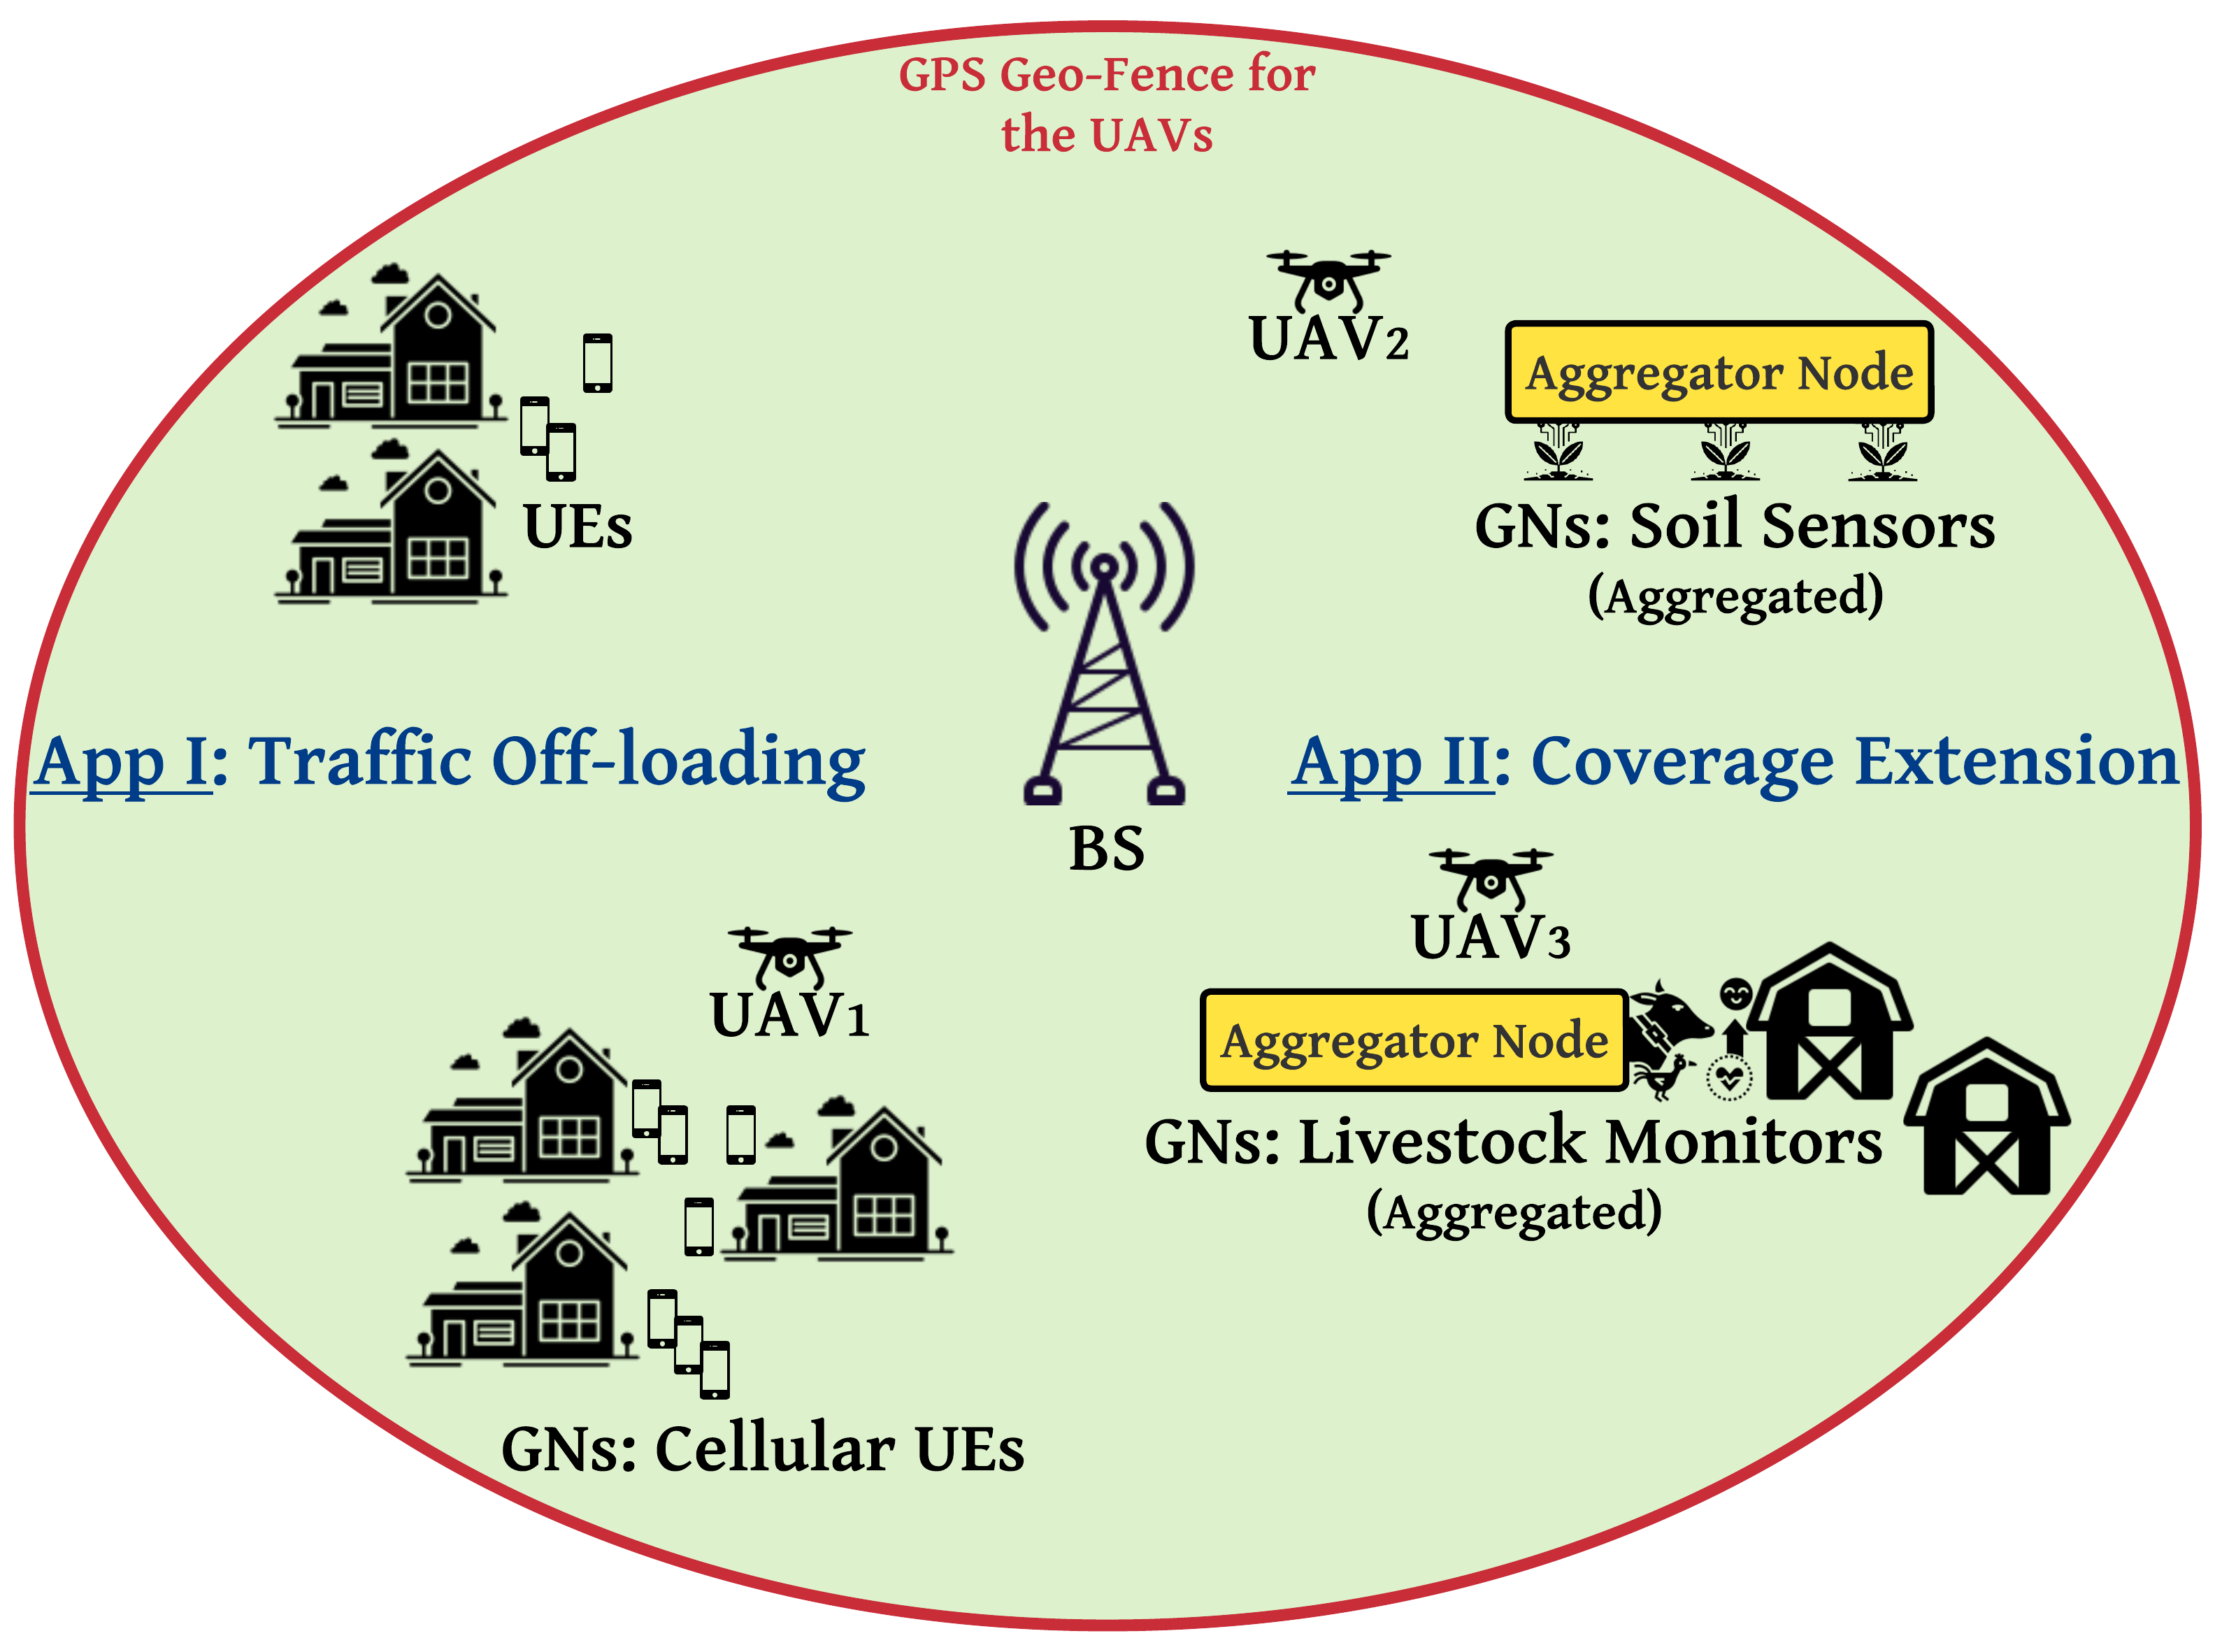
\includegraphics[width=0.9\linewidth]{figs/Deployment_Model.png}
         \caption{Deployment Model}
         \label{F1}
     \end{subfigure}
     \begin{subfigure}{0.496\linewidth}
         \centering
         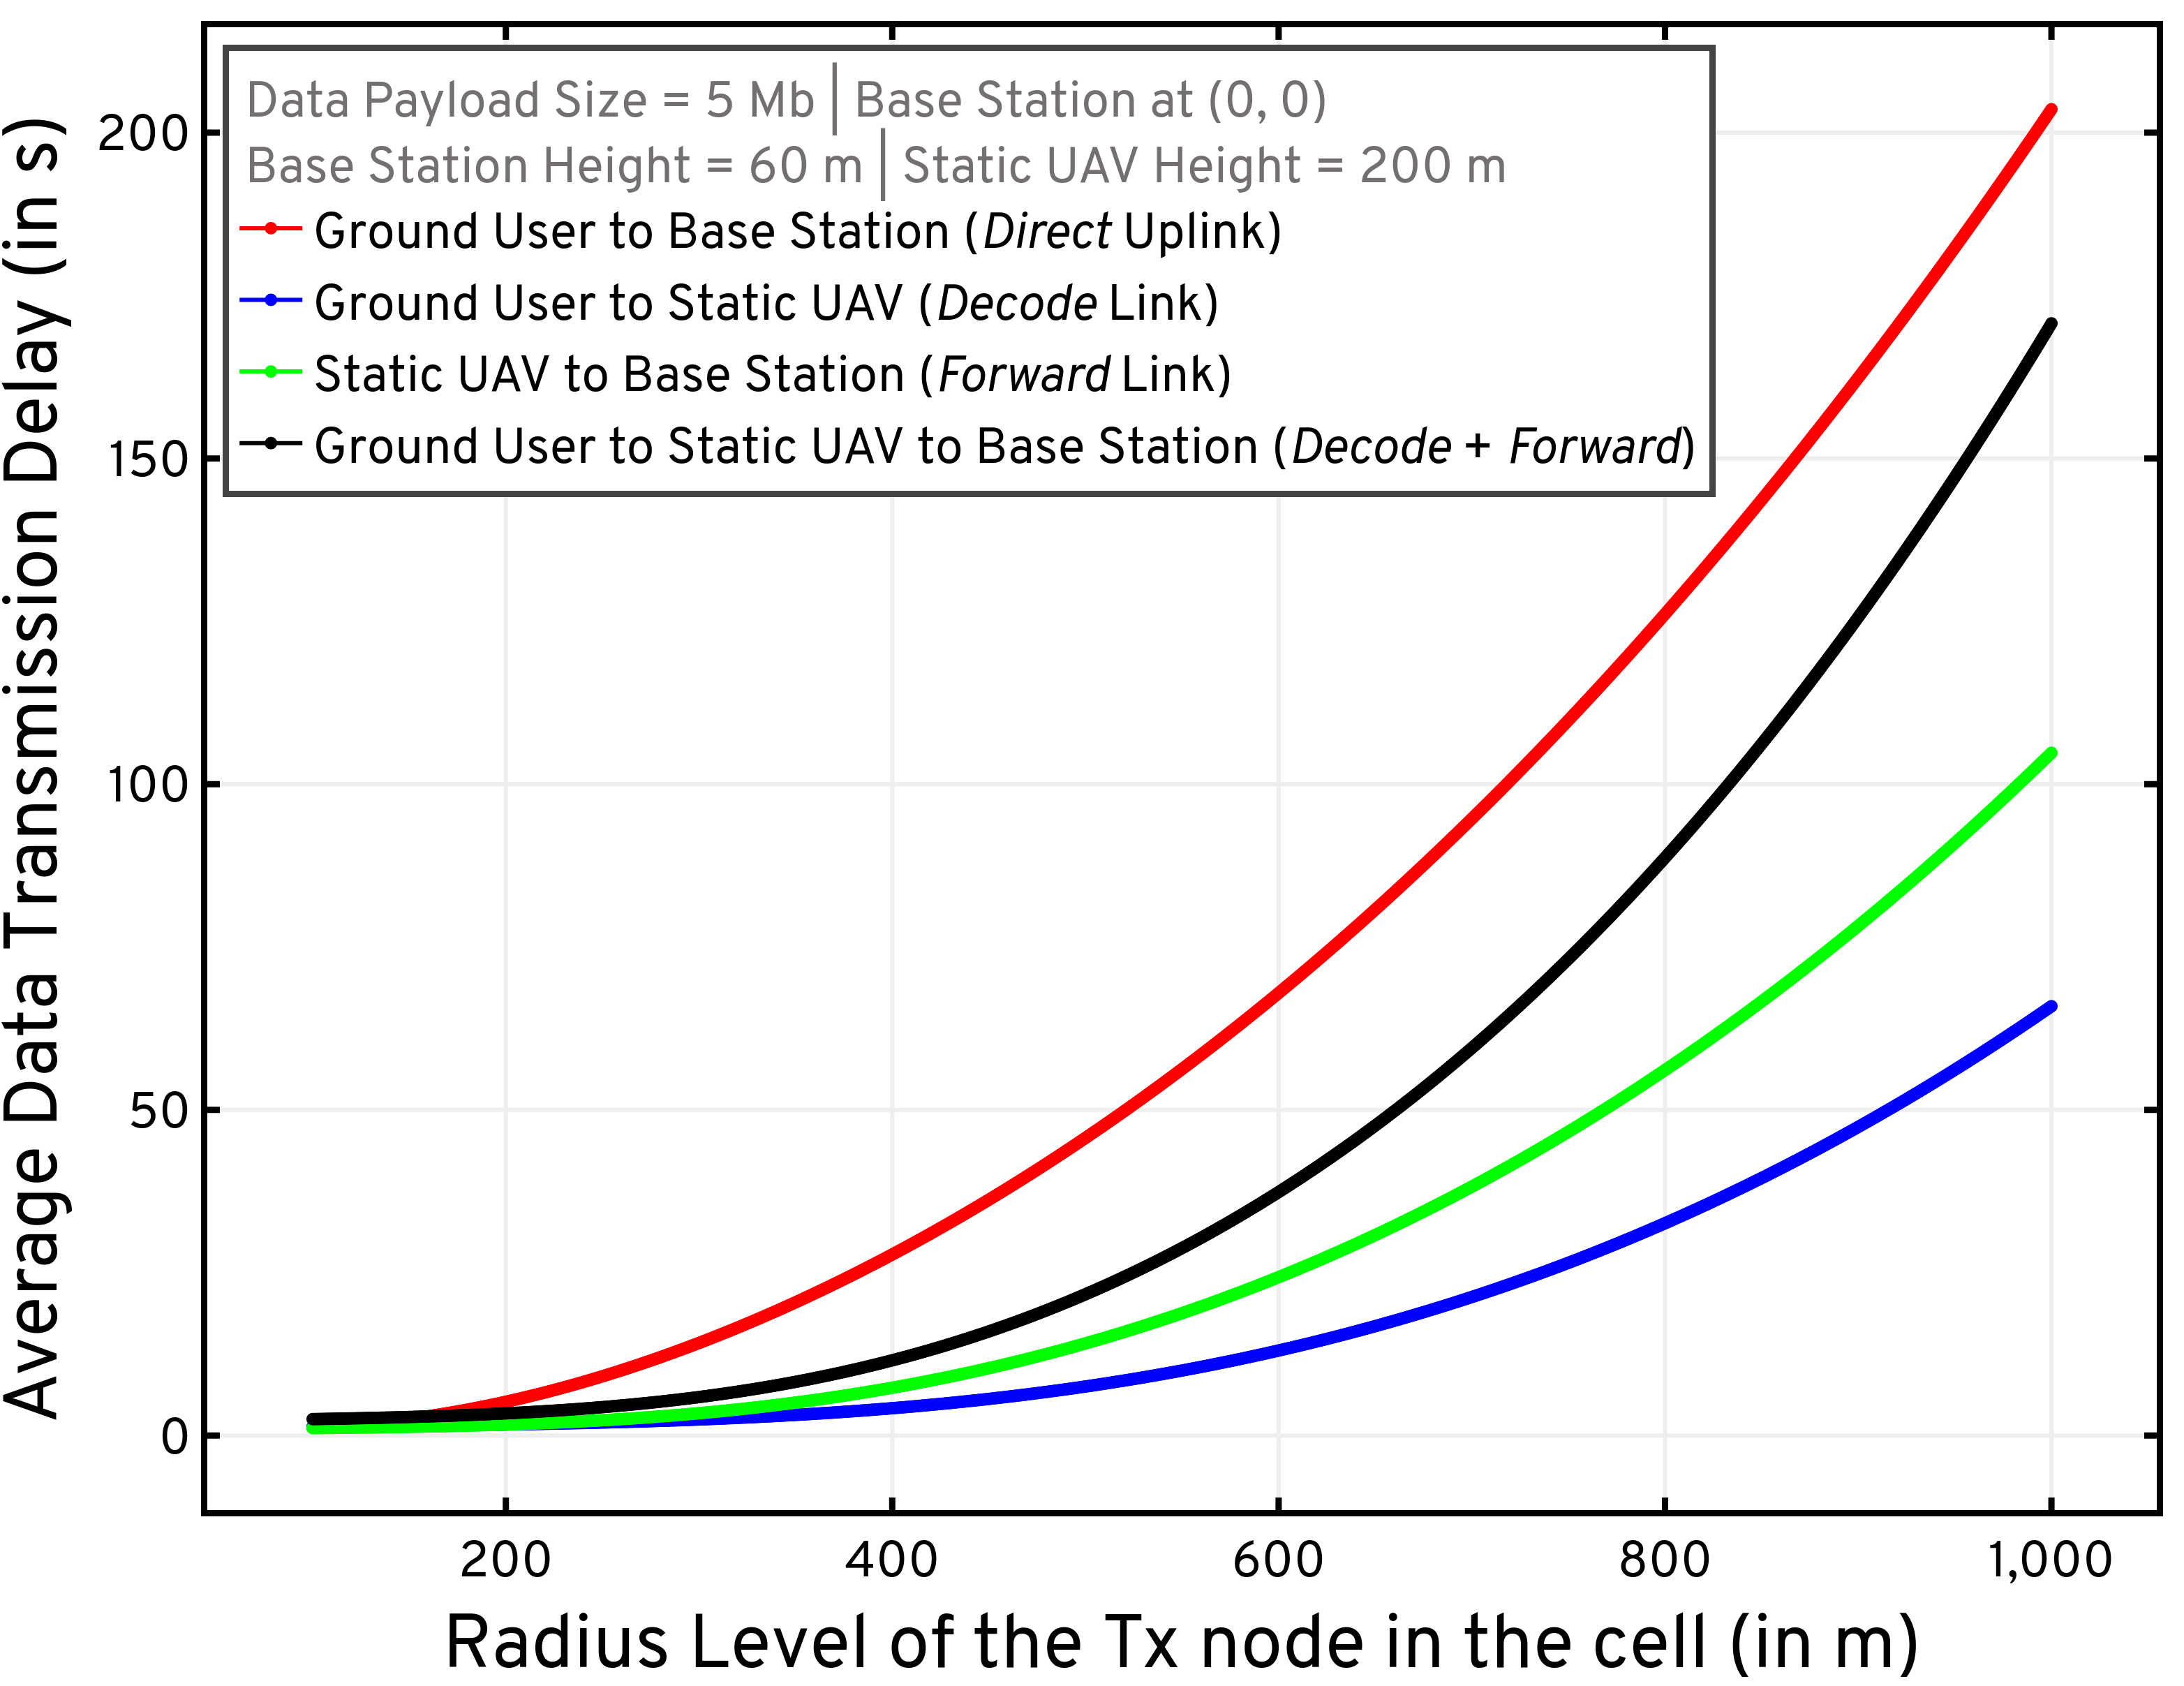
\includegraphics[width=0.9\linewidth]{figs/Channel_Model.png}
         \caption{Channel Model}
         \label{F2}
     \end{subfigure}
     \vspace{-2mm}
     \caption{(a) A terrestrial BS aided by $3$ UAVs serving as cellular relays for a diverse set of GNs: traffic offloading for cellular UEs, and coverage extensions for livestock monitors and soil sensors; (b) The service latencies experienced by GNs for $5$ Mb data payloads under both direct-BS as well as Decode-and-Forward strategies.}
     \label{F1andF2}
\end{figure}

\noindent{\textbf{A2G Channel Model}}: For a generic link, we denote the flat-fading channel coefficient as $h{\triangleq}\sqrt{\beta}g$, where $\beta$ captures the large-scale channel variations, and $g$ with $\mathbb{E}\left[|g|^2\right]{=}1$ is the small-scale fading component. We model the large-scale component as $\beta{=}\beta_{\mathrm{LoS}}(d){\triangleq}\beta_{0}d^{-\alpha}$ for line-of-sight (LoS) and $\beta{=}\beta_{\mathrm{NLoS}}(d){\triangleq}\kappa\beta_{0}d^{-\tilde{\alpha}}$ for non-LoS (NLoS) links, where $\beta_{0}$ is the pathloss referenced at a distance of $1$ meter, $2{\leq}\alpha{\leq}\tilde{\alpha}$ are the LoS and NLoS path-loss exponents, $\kappa{\in}(0,1]$ captures the additional NLoS attenuation, and $d$ denotes the Tx-Rx Euclidean distance \cite{SCA}.

\noindent{We} model the LoS and NLoS probabilities as functions of the elevation angle $\varphi{\in}(0^{o},90^{o}]$, i.e., 
\begin{align}\label{eq:PLoS}
	&P_{\mathrm{LoS}}(\varphi)=\frac{1}{1+z_{1}\exp\left(-z_{2}\left[\varphi-z_{1}\right]\right)},\;\;
	P_{\mathrm{NLoS}}(\varphi)=1-P_{\mathrm{LoS}}(\varphi),
\end{align}
where $z_{1}$ and $z_{2}$ are parameters specific to the propagation environment (e.g., rural, suburban, and urban) \cite{LAP}. The distribution of the small-scale fading component $g$ also depends on the LoS or NLoS link state \cite{WCBook}. Specifically, for a LoS link, as in \cite{Rician}, we model $g$ as Rician fading with a $\varphi$-dependent $K$-factor $K(\varphi){=}k_{1}\exp\left(k_{2}\varphi\right)$, where coefficients $k_{1}$ and $k_{2}$ are determined by the propagation environment \cite{Rician}. For a NLoS link, we model $g$ as Rayleigh fading \cite{WCBook} (Rician with $K{=}0$). Given $h$, the link capacity is $C(h){=}B{\cdot}\log_{2}\left(1{+}\frac{|h|^{2}P}{N_{0}B\Gamma} \right)$, where $P$ is the transmission power, $N_{0}$ is the noise power spectral density at the receiver, $B$ is the channel bandwidth, and $\Gamma$ is the Signal-to-Noise Ratio (SNR) gap between practical modulation-and-coding schemes and theoretical Gaussian signaling \cite{Rician}. We assume that other sources of signal degradation, such as the Doppler effect, are well-compensated at the receiver (e.g., see the approaches in \cite{Doppler}). 

Since the large-scale components typically vary slowly relative to the rate of acquisition of Channel State Information (CSI), we assume that the current large-scale parameters $(\beta,K)$ are known at the transmitter's side throughout the communication process, which enables rate-control at the transmitter; on the other hand, small-scale fading conditions vary at a much faster timescale, hence cannot be tracked at the transmitter, which may result in outages when the selected rate exceeds the channel capacity $C(h)$. Thus, given $(\beta,K)$ and a transmission rate of $\Upsilon$ [bits per second], we define the outage probability $P_{\mathrm{out}}(\Upsilon,\beta,K) \triangleq \mathbb{P}(C(\sqrt{\beta}g){<}\Upsilon)|\beta,K) = \mathbb{P}\left(|g|^{2}{<}u(\Upsilon,\beta)\right)$, where $u(\Upsilon,\beta){\triangleq}N_{0}B\Gamma(2^{\Upsilon/B}{-}1)/(\beta P)$. Since $2(K{+}1)|g|^{2}$ has a non-central $\chi^2$ distribution with $2$ degrees of freedom and non-centrality parameter $2K$, we find that
\begin{align}
	P_{\mathrm{out}}(\Upsilon,\beta,K)=1-Q_{1}\left(\sqrt{2K},\sqrt{2(K+1)u(\Upsilon,\beta)}\right),
\end{align}
where $Q_{1}(\cdot,\cdot)$ is the standard Marcum $Q$-function \cite{Rician}. Note that when $K{=}0$ (Rayleigh fading for NLoS links), the function specializes to $Q_{1}\left(0,\sqrt{2u(\Upsilon,\beta)}\right){=}\exp(-u(\Upsilon,\beta))$. We assume that the small-scale fading is averaged out across time, yielding the expected throughput as,
\begin{align}
	R(\Upsilon,\beta,K)=\Upsilon\cdot\left(1-P_{\mathrm{out}}(\Upsilon,\beta,K)\right)=\Upsilon\cdot Q_{1}\left(\sqrt{2K},\sqrt{2(K+1)u(\Upsilon,\beta)}\right).
\end{align}
In our model, we permit rate adaptation at the transmitter based on the large-scale parameters $(\beta,K)$, coordinated through the control channel via CSI feedback. The transmission rate $\Upsilon$ is chosen to maximize the expected throughput given $(\beta,K)$, i.e., $\Upsilon^{*}(\beta,K){\triangleq}\argmax_{\Upsilon{\geq}0}R(\Upsilon,\beta,K).$ To solve this problem, let $Z{\triangleq}\sqrt{\frac{2{\beta}P}{N_{0}B\Gamma}u(\Upsilon,\beta)}$, so that $\Upsilon{=}B\log_{2}\left(1{+}\frac{1}{2}Z^{2}\right){\triangleq}f(Z)$. It follows that $\Upsilon^{*}(\beta,K){=}f(Z^{*}(\beta,K))$, where $Z^{*}(\beta,K)\triangleq\argmin_{Z{\geq}0}h(Z)$ and $h(Z) \triangleq -\ln f(Z) - \ln Q_{1}\left(\sqrt{2K},\sqrt{\frac{(K{+}1)\beta P}{N_{0}B\Gamma}}Z\right)$. Since the function $h(Z)$ is convex, $Z^{*}(\beta,K)$ can be found efficiently using a bisection method. Upon determining the optimal transmission rate $\Upsilon^{*}(\beta,K)$, we define the optimized throughput, as a function of the large-scale conditions, as $R^{*}(\beta,K) \triangleq R(\Upsilon^{*}(\beta,K),\beta,K)$. Further assuming that the LoS and NLoS conditions are averaged out in the temporal and spatial dimensions, the average link throughput with rate adaptation is
\begin{align}\label{TBar}
	\bar{R}(d,\varphi)\triangleq P_{\mathrm{LoS}}(\varphi)\cdot R^{*}(\beta_{\mathrm{LoS}}(d),K(\varphi))+P_{\mathrm{NLoS}}(\varphi)\cdot R^{*}(\beta_{\mathrm{NLoS}}(d),0).
\end{align}
This throughput is then specialized to the three distinct communication links by expressing the transmission powers, the environment-specific parameters ($z_{1}$, $z_{2}$, $k_{1}$, $k_{2}$), the large-scale parameters $(\beta,K)$, and the LoS or NLoS probabilities \eqref{eq:PLoS} based on the spatial configuration, i.e., $d$ and $\varphi$.
Specifically, for the GN$\rightarrow$BS link, we let $\bar{R}_{GB}(r)$ be the throughput with the GN in position $(r,\theta)$, computed by setting the GN-BS distance as $d{=}\sqrt{H_{B}^{2}{+}r^{2}}$ and the elevation angle as $\varphi{=}\sin^{-1}\left(H_{B}/d\right)$ in \eqref{TBar}. Similarly, for the GN$\rightarrow$UAV link, we let $\bar{R}_{GU}(r_{GU})$ be the throughput when the GN-UAV distance (projected onto the $x{-}y$ plane) is $r_{GU}$, computed by setting the GN-UAV Euclidean distance as $d{=}\sqrt{r_{GU}^{2}{+}H_{U}^{2}}$ and the elevation angle as $\varphi{=}\sin^{-1}\left(H_{U}/d\right)$ in \eqref{TBar}. Finally, for the UAV$\rightarrow$BS link, we let $\bar{R}_{UB}(r_{UB})$ be the throughput when the $x{-}y$ projected UAV-BS distance is $r_{UB}$, computed by setting the GN-UAV Euclidean distance as $d{=}\sqrt{r_{UB}^{2}{+}(H_{U}{-}H_{B})^{2}}$ and the elevation angle as $\varphi{=}\sin^{-1}\left((H_{U}{-}H_{B})/d\right)$ in \eqref{TBar}. As depicted in Fig. \ref{F2}, in a system with the rate adaptation capabilities described above, the poor QoS performance experienced by GNs farther away from the BS---due to the deterioration in LoS probabilities with distance---motivates the need for aerial relays to ensure QoS guarantees.

\noindent{\textbf{UAV Mobility Power Model}}: For a rotary-wing UAV, since its communication power needs ($\approx$\qty[mode=text]{5}{\watt}) are dwarfed by its mobility power requirements ($\approx$\qty[mode=text]{1000}{\watt}), we model the on-board energy constraints of the UAV purely in terms of its flight power. From \cite{SCA}, we have that
\begin{align}\label{eq:Power}
    P_{\mathrm{mob}}(V)=P_{1}\left(1+\frac{3V^{2}}{U_{\mathrm{tip}}^{2}}\right)+P_{2}\left(\sqrt{1+\frac{V^{4}}{4v_{0}^{4}}}-\frac{V^{2}}{2v_{0}^{2}}\right)^{1/2}+P_{3}V^{3},
\end{align}
where $V$ is the horizontal flying velocity, $P_{j},j{\in}\{1,2,3\}$ are scaling constants, $U_{\mathrm{tip}}$ is the rotor blade tip velocity, and $v_{0}$ is the mean rotor induced velocity while hovering. From \cite{SCA}, hovering requires \qty[mode=text]{1370}{\watt}, whereas flying at the power-minimizing velocity of \qty[mode=text]{22}{\meter\per\second} only consumes \qty[mode=text]{940}{\watt}. This suggests that, as we will show, the mobility of the UAVs can be exploited to reduce their power consumption, while simultaneously ensuring that the QoS mandates for GNs in the cell are successfully met. Hence, our objective is to solve for an energy-conscious adaptive service scheduling and trajectory optimization scheme wherein a distributed swarm of UAV relays are employed to minimize the time-average communication service delay experienced by GNs in the cell, randomly generating uplink transmission requests, subject to an average per-UAV mobility power constraint. To this end, in the next section, we formulate a framework specialized to single UAV deployments, which is then extended to UAV swarms in Sec. \ref{S5}.
\vspace{-4mm}


\section{MAESTRO: A Semi-Markov Decision Process Formulation}\label{S3}
\vspace{-2mm}

In this section, we specialize the deployment, communication, and channel models detailed in Sec. \ref{S2} to single UAV relay settings. Accordingly, we describe the mathematical constructions involved in the design of our solution framework to minimize the time-average service delay experienced by the GNs in the cell, subject to an average UAV mobility power constraint via a Semi-Markov Decision Process (SMDP) formulation. The effective traffic rate experienced by a single UAV is $\Lambda'{\triangleq}\frac{\Lambda}{N_U}$ [requests per unit time per UAV], which is assumed in this section in place of the overall rate $\Lambda$. Let $\mathbf{q}_{U}(t){=}(r_{U}(t),\theta_{U}(t))$ be the polar coordinate of the UAV at time $t$, projected onto the $x{-}y$ plane, where $r_{U}(t){\in}\mathbb{R}_{+}$ and $\theta_{U}(t){\in}[0,2\pi)$ denote the UAV's radius and angle with respect to the BS (cell center). This specialized setup is illustrated in Fig. \ref{F4}.

We note that the operations of the UAV relay can be split into the following phases. In the waiting phase, no GN requests are being served by the UAV, which thus moves according to a {waiting policy}, until a new request is received. When a new GN request is received, say from position $(r,\theta)$, the system transitions to the request scheduling phase, where it is determined whether the GN should transmit its data payload directly to the BS, or relay it through the UAV. If direct transmission is selected, the system immediately re-enters the waiting phase, as the UAV remains free to serve other requests; else, the system enters the UAV relay phase, in which the GN relays its data payload through the UAV using the D\&F protocol; upon the completion of this relay service, the system re-enters the waiting phase. Note that the BS can accommodate simultaneous transmissions using orthogonal channels (see Sec. \ref{S2}): therefore, new requests received during the UAV relay phase are directly served by the BS.  In this section, we assume that there are always channels available, so that these requests can be immediately served by the BS; the effect of the limited number of channels is studied in Sec. \ref{S5} via queuing models.

\begin{figure} [t]
    \centering
    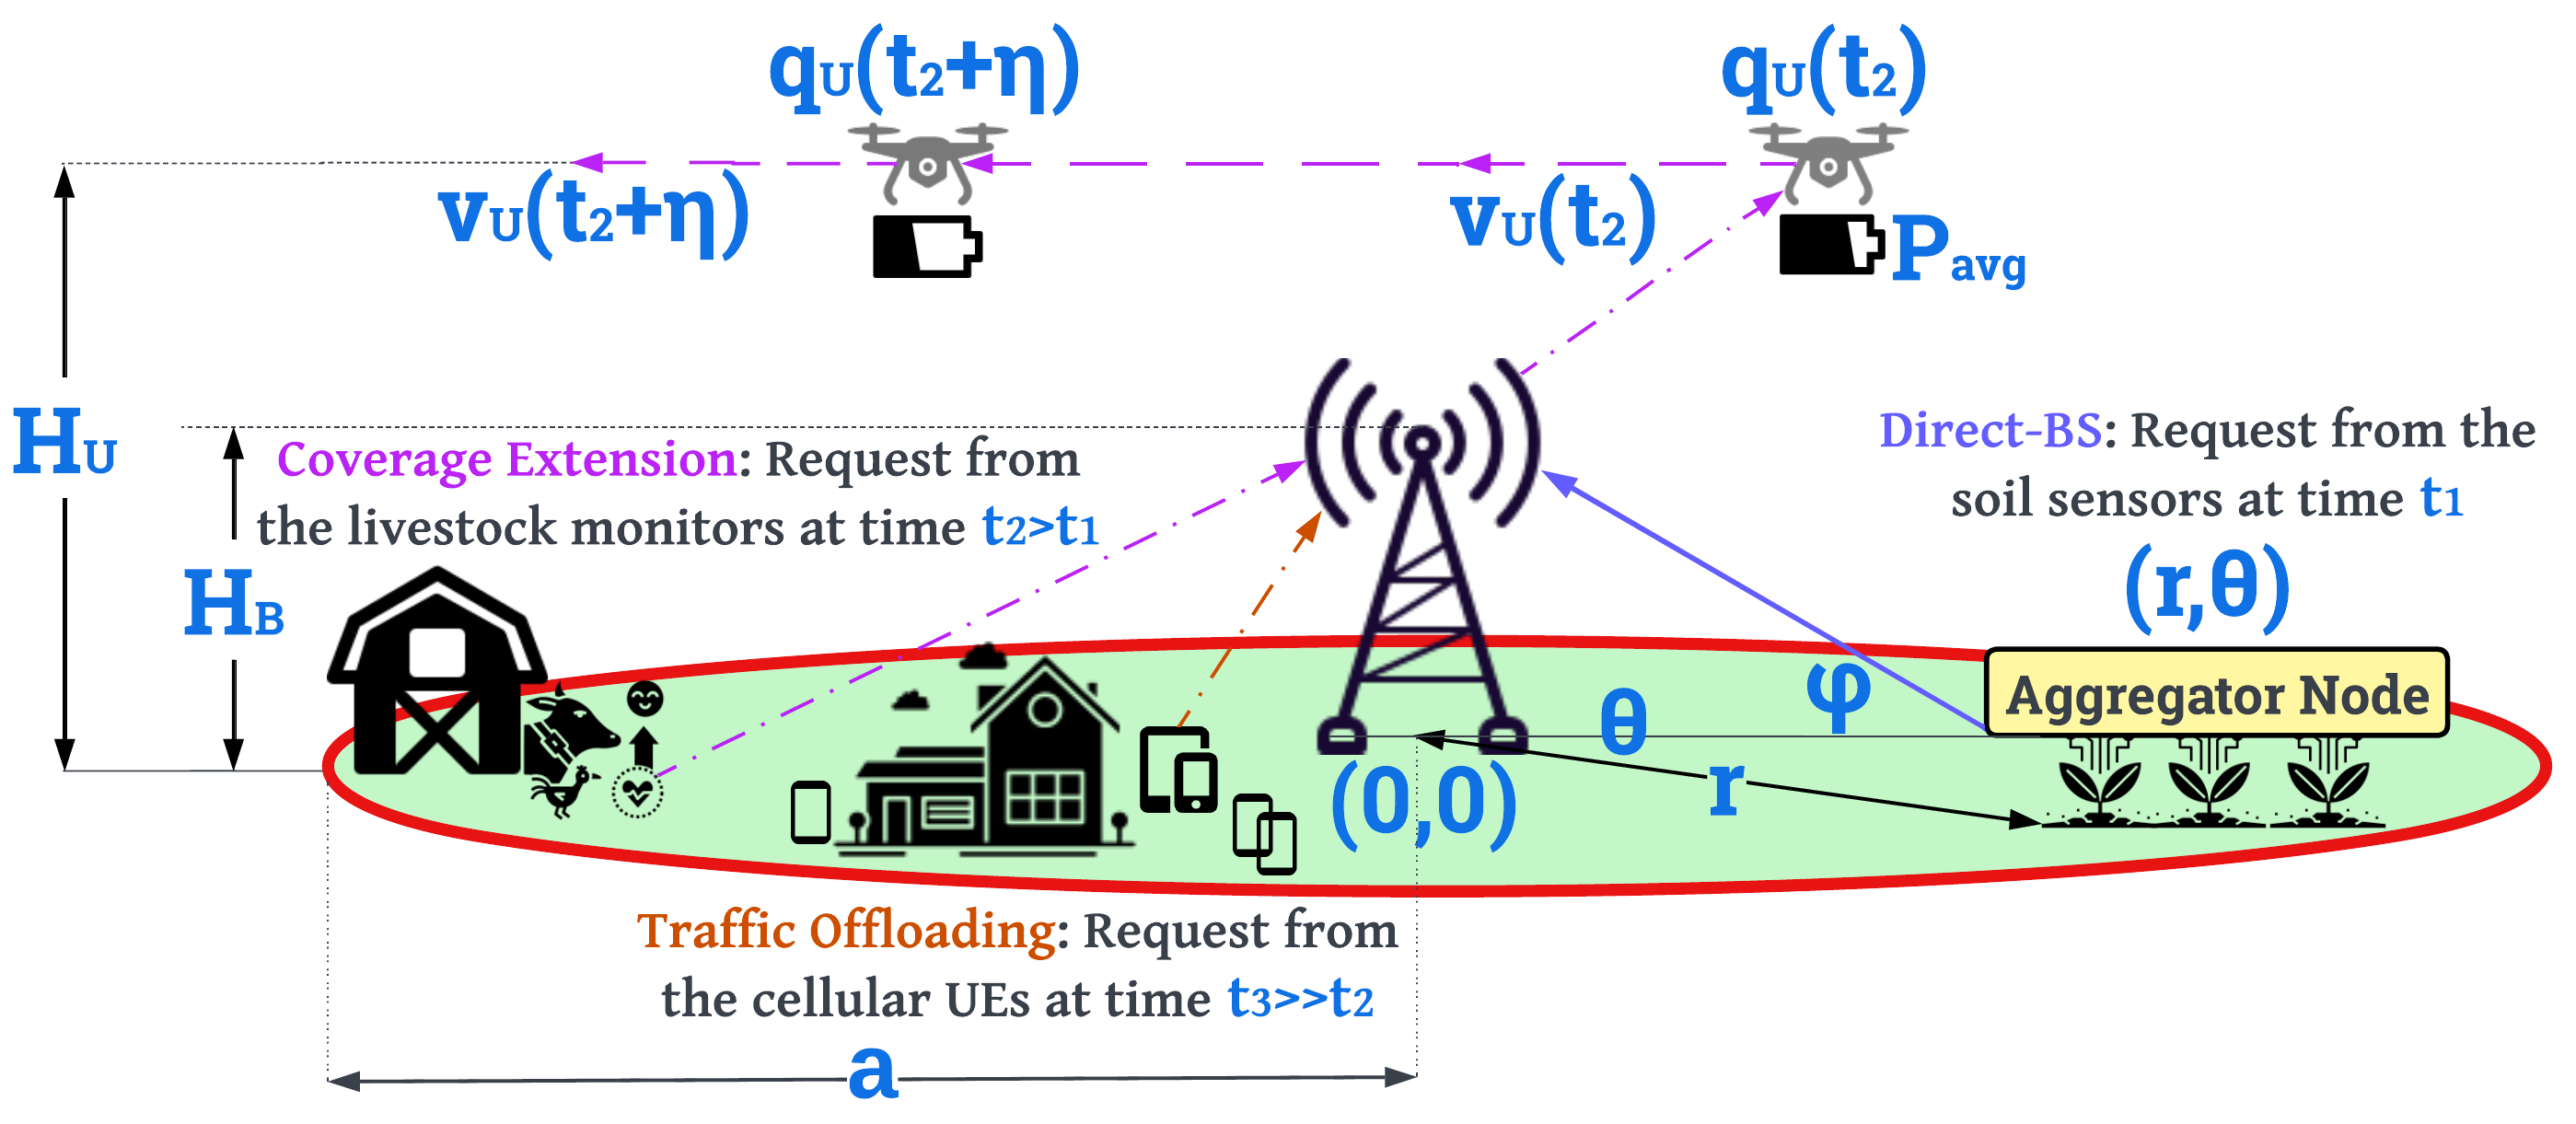
\includegraphics[width=0.7\linewidth]{figs/Single_Agent_Specialization.png}
    \vspace{-2mm}
    \caption{The single-agent specialization of our generalized deployment depicted in Fig. \ref{F1}.}
    \label{F4}
\end{figure}

Next, we formulate the average communication delay and UAV energy consumption under a given policy $\mu$ that defines the request scheduling, communication strategy, and UAV trajectory (formally defined later). We define a decision interval as the time duration spanning the start of a {waiting} phase, the subsequent {request scheduling} phase when a GN request is received, until the system re-enters the {waiting} phase after scheduling a direct transmission to the BS, or following the {UAV relay} phase. Consider the $u$th such decision interval; let $\Delta_{u}^{(w)}$ be the time to wait for a new request, and $\Delta_{u}^{(s)}$ be the time to serve it, either through the BS (denoted with the scheduling decision $\xi_{u}{=}0$) or through the UAV ($\xi_{u}{=}1$). Then, the $u$th decision interval duration is $\Delta_{u}{=}\Delta_{u}^{(w)}{+}\xi_{u}\Delta_{u}^{(s)}$, since the UAV enters the {waiting phase} immediately if a direct transmission to the BS is scheduled. Let $N_{u}{\geq}0$ be the number of additional requests received during the UAV relay phase of the $u$th decision period; since these additional requests are served directly by the BS, let $\Delta_{u,i}^{(bs)},i=\{1,{\dots},N_{u}\}$ be their communication delays. Let $E_{u}$ be the UAV mobility energy expended during the $u$th decision interval. Let $M_{t}$ be the total number of decision intervals completed up to time $t$. We define $\bar{D}_{\mu}$, the expected average communication delay per GN request under $\mu$, as the total communication delay accrued until time $t$, over the total number of requests served until time $t$; similarly, we define $\bar{P}_{\mu}$, the expected average UAV power, as the total energy consumption over the total duration of the $M_{t}$ intervals up to time $t$, i.e.,
\begin{align}\label{eq:DBarMu}
    &\bar{D}_{\mu} \triangleq \lim_{t \rightarrow \infty} \mathbb{E}_{\mu} \Bigg[
    \frac{\frac{1}{M_t}\sum_{u = 1}^{M_t}(\Delta_u^{(s)}+\xi_u\sum_{i=1}^{N_u}\Delta_{u,i}^{(bs)})}{
    \frac{1}{M_t}\sum_{u = 1}^{M_t}(1+\xi_uN_u)
    }\Bigg],\ 	\bar{P}_{\mu} \triangleq \lim_{t \rightarrow \infty} \mathbb{E}_{\mu} \Bigg[ \frac{\frac{1}{M_t}\sum_{u = 1}^{M_t}E_u}{\frac{1}{M_t}\sum_{u = 1}^{M_t} \Delta_u}\Bigg].
\end{align}
Note that $\bar{D}_{\mu}$ in \eqref{eq:DBarMu} captures the delays of all requests, i.e., those relayed through the UAV ($\xi_{u}{=}1$), those transmitted directly to the BS ($\xi_{u}{=}0$), as well as the $N_{u}$ additional requests served directly by the BS during the UAV relay phase.
The goal is to solve $\bar{D}_{\mu}^{*}{=}\underset{\mu}{\mathrm{min}}\bar{D}_{\mu}\text{ s.t. }\bar{P}_{\mu}{\leq}P_{\mathrm{avg}}$, with optimal policy $\mu^{*}$. To simplify these expressions, let
$\bar{\mathbb{E}}_{\mu}[C_u]\triangleq\lim\limits_{t \rightarrow \infty} \mathbb{E}_{\mu}
[\frac{1}{M_t} \sum_{u = 1}^{M_t }C_u]$ be a shorthand notation to denote the long-term average cost $C_u$ per decision interval, and let
$\bar{E}_{\mu}{\triangleq}\bar{\mathbb{E}}_{\mu} \left[E_u\right],\ \bar{T}_{\mu}{\triangleq}\bar{\mathbb{E}}_{\mu} \left[\Delta_u\right],\ \bar{N}_{\mu}{\triangleq}\bar{\mathbb{E}}_{\mu} \left[1+\xi_uN_u\right],\ \bar{W}_{\mu}^{(s)}{\triangleq}\bar{\mathbb{E}}_{\mu}\left[\Delta_u^{(s)}\right],\ \bar{W}_{\mu}^{(bs)}{\triangleq}\bar{\mathbb{E}}_{\mu}[\xi_u\sum_{i=1}^{N_u}\Delta_{u,i}^{(bs)}]$ be the expected average UAV energy expenditure ($\bar{E}_{\mu}$), duration ($\bar{T}_{\mu}$), number of requests served ($\bar{N}_{\mu}$), delay of requests for which a scheduling decision is made ($\bar{W}_{\mu}^{(s)}$), and total delays of requests served directly by the BS during the UAV relay phase
($\bar{W}_{\mu}^{(bs)}$), per decision interval. 
Since $\bar{P}_{\mu}{=}\bar{E}_{\mu}/\bar{T}_{\mu}$ and $\bar{D}_{\mu}{=}(\bar{W}_{\mu}^{(s)}+\bar{W}_{\mu}^{(bs)})/\bar{N}_{\mu}$ from Little's Law \cite{LittlesLaw},
we can then reformulate
\begin{align}\label{eq:OverallObj1}
    &\bar{D}_{\mu}^{*} = \underset{\mu}{\mathrm{min}} \; 
	\frac{\bar{W}_{\mu}^{(s)}+\bar{W}_{\mu}^{(bs)}}{\bar{N}_{\mu}}\;\;
	\mathrm{s.t.} \; \bar{E}_{\mu}-P_{\mathrm{avg}}\bar{T}_{\mu}\leq 0.
\end{align}

Let $\mu_{BS}$ denote the policy wherein all requests are served by the BS and the UAV flies around at the power-minimizing speed $V_{\mathrm{min}}$. Clearly, this policy is feasible for the above problem, since the UAV uses minimum flying power.
Since the delay to serve a request from a GN in position $(r,\theta)$ by direct transmission to the BS is $L/\bar R_{GB}(r)$,  the expected delay under policy $\mu_{BS}$ is obtained by computing the expectation with respect to the radial coordinate, $\bar{D}_{BS}{\triangleq}\int_{0}^{a}\frac{L}{\bar{R}_{GB}(r)}f_{R}(r)\mathrm{d}r$. Clearly, by optimizing over $\mu$, $\bar{D}_{\mu}^{*}{\leq}\bar{D}_{BS}$: this suggests that optimization of the UAV trajectory and scheduling decisions is key to improving the delay performance to serve requests. Note the inherent complexity that is required to solve the optimization problem \eqref{eq:OverallObj1}: as the policy varies, the delay metric changes both the numerator and denominator terms of the objective function, which cannot be solved with standard dynamic programming algorithms. To address this challenge, we now propose an alternative optimization criterion based on upper- and lower-bounds to $\bar{D}_{\mu}$.

Let $\bar{W}_{\mu}{\triangleq}\bar{W}_{\mu}^{(s)}{+}\bar{W}_{\mu}^{(bs)}$. If $\xi_u{=}1$, then additional requests received during the UAV relay phase are served directly by the BS, with delay $L/\bar{R}_{GB}(r)$ for a GN in position $(r,\theta)$. Therefore, the expected average communication delay to serve these additional requests is $\mathbb E[\Delta_{u,i}^{(bs)}]{=}\bar{D}_{BS}$, yielding $\bar{W}_{\mu}{=}\bar{W}_{\mu}^{(s)}{+}\bar{D}_{BS}(\bar{N}_{\mu}{-}1)$ and
 $\bar{D}_{\mu}{=}\frac{\bar{W}_{\mu}}{\bar{N}_{\mu}}{=}\frac{\bar{W}_{\mu}^{(s)}}{\bar{N}_{\mu}}{+}\left(1{-}\frac{1}{\bar N_{\mu}}\right)\bar{D}_{BS}$. 
 Let $\mu$ be any policy (including the optimal one) that satisfies $\bar{D}_{\mu}{\leq}\bar{D}_{BS}$: under such policy, since $\bar{N}_{\mu}{\geq}1$, the expression above implies that $\bar{W}_{\mu}^{(s)}{\leq}\bar{D}_{\mu}{\leq}\bar{D}_{BS}$. 
Moreover, since
$\mathbb{E}[N_{u}|\Delta_{u}^{(s)}]{=}\Delta_{u}^{(s)}\Lambda'$ and $\xi_{u}{\leq}1$, it follows that $\bar{N}_{\mu}{\leq}1{+}\Lambda'\bar{W}_{\mu}^{(s)}$
with  equality if the UAV always serves requests. 
This implies that $\bar{W}_{\mu}^{(s)}{\leq}\bar{D}_{\mu}{\leq}\bar{W}_{\mu}^{(s)}\frac{1{+}\Lambda'\bar{D}_{BS}}{1{+}\Lambda'\bar{W}_{\mu}^{(s)}}{\leq}\bar{D}_{BS}$. 
% Therefore, under the optimal policy, we must have $\bar{D}_{\mu}^{*}{\leq}\bar{D}_{\mu_{BS}}{=}\bar{D}_{BS}$. Since $\bar{N}_{\mu}{\geq}1$, this implies that $\bar{W}_{\mu^*}^{(s)}{\leq}\bar{D}_{BS}$. Let $\mu$ be any policy (including the optimal one) that satisfies $\bar{W}_{\mu}^{(s)}{\leq}\bar{D}_{BS}$: under such policy, $\bar{W}_{\mu}^{(s)}{\leq}\bar{D}_{\mu}{\leq}\bar{D}_{BS}$. 
Observing that both the lower and upper bounds of $\bar{D}_{\mu}$ are increasing functions of $\bar{W}_{\mu}^{(s)}$, we
replace \eqref{eq:OverallObj1} with the surrogate 
 $\underset{\mu}{\mathrm{min}}\bar{W}_{\mu}^{(s)}\mathrm{ s.t. }\bar{E}_{\mu}{-}P_{\mathrm{avg}}\bar{T}_{\mu}{\leq}0,$ which will be the focus of our subsequent analyses. To solve this, we employ the Lagrangian
\begin{align}\label{eq:W2Lagr}
    &g(\nu){=}\underset{\mu}{\mathrm{min}} \left( \bar{W}_{\mu}^{(s)} + \nu (\bar{E}_{\mu}-P_{\mathrm{avg}}\bar{T}_{\mu}) \right)
    {=}\underset{\mu}{\mathrm{min}}\, \lim_{t \rightarrow \infty} \, \mathbb{E}_{\mu} \left[\frac{1}{M_t} \sum_{u = 1}^{M_t}\left( \Delta_u^{(s)} + \nu (E_u - P_{\mathrm{avg}}\Delta_u) \right) \right],\!\!
\end{align}
where $\nu$ is the dual variable, optimized by solving $\max_{\nu{\geq}0}g(\nu)$. We now demonstrate that for a given $\nu{\geq}0$, \eqref{eq:W2Lagr} can be cast as a Semi-Markov Decision Process (SMDP) and solved with dynamic programming tools: next, we discuss its states, actions, transitions, and policy. 

\noindent{\textbf{States}}: The state is defined by the UAV position $\mathbf{q}_{U}$, an element of the set $\mathcal{Q}_{\mathrm{UAV}}{\triangleq}\mathbb{R}_{+}{\times}[0,2\pi)$ (polar coordinates), and the position of the GN originating traffic $\mathbf{q}_G$, taking values from the set  $\mathcal{Q}_{\mathrm{GN}}{\triangleq}[0,a]{\times}[0,2\pi)$. The state space is then $\mathcal{S}{=}\mathcal{S}_{\mathrm{wait}}{\cup}$ $\mathcal{S}_{\mathrm{comm}}$, where $\mathcal{S}_{\mathrm{wait}}{=}\mathcal{Q}_{\mathrm{UAV}}$ is the set of {waiting} states and $\mathcal{S}_{\mathrm{comm}}{=}\mathcal{Q}_{\mathrm{UAV}}{\times}\mathcal{Q}_{\mathrm{GN}}$ is the set of {communication} states. Crucial to the definition of the SMDP is how the system is sampled in time to define Markovian dynamics in the evolution of the sampled states: accordingly, we define the actions available in each state $\mathbf{s}{\in}\mathcal{S}$ and the transition probabilities, along with the time duration $T(\mathbf{s};\mathbf{a})$, the UAV energy usage $E(\mathbf{s};\mathbf{a})$, and the request service delay $\Delta(\mathbf{s};\mathbf{a})$ metrics accrued in state $\mathbf{s}$ under action $\mathbf{a}$.

\noindent{\textbf{Waiting states' actions, transitions, and metrics}}: If the UAV is in {waiting} state $\mathbf{s}_{n}{=}\mathbf{q}_{U}{\in}\mathcal{S}_{\mathrm{wait}}$ at time $t$, i.e., it is in position $\mathbf{q}_{U}(t){=}\mathbf{q}_{U}{=}(r_{U},\theta_{U})$ with no active requests, then the actions available are to move the UAV with radial and angular velocity components $(v_{r},\theta_{c})$, over an arbitrarily small duration $\Delta_{0}{\ll}1/\Lambda'$. Under a maximum velocity constraint $V_{\mathrm{max}}$, this waiting-state action space is given by $\mathcal{A}_{\mathrm{wait}}(r_{U}){\triangleq}\Big\{(v_{r},\theta_{c}){\in}\mathbb{R}^{2}\Big|\sqrt{v_{r}^{2}{+}r_{U}^{2}{\cdot}\theta_{c}^{2}}{\leq}V_{\mathrm{max}} \Big\}$, where $v_{U}{=}\sqrt{v_{r}^{2}{+}r_{U}^{2}\theta_{c}^{2}}$ is the velocity expressed with respect to polar coordinates. Upon choosing action $\mathbf{a}{=}(v_{r},\theta_{c}){\in}\mathcal{A}_{\mathrm{wait}}(r_{U})$, the communication delay is $\Delta(\mathbf{s};\mathbf{a}){=}0$, since there is no ongoing communication; the duration of a waiting state visit is $T(\mathbf{s};\mathbf{a}){=}\Delta_{0}$, during which the UAV uses an amount of energy $E(\mathbf{s};\mathbf{a}){=}\Delta_{0}P_{\mathrm{mob}} \left(v_{U}\right)$ to move at velocity $v_{U}$. The new state is then sampled at time $t{+}\Delta_{0}$, with the UAV moved to the new position $\mathbf{q}_{U}(t{+}\Delta_{0}){\approx}(r_{U},\theta_{U}){+}(v_{r},\theta_{c})\Delta_{0}$. With probability $e^{-\Lambda'\Delta_{0}}$, no new request is received in the time interval $[t,t{+}\Delta_{0}]$, so that the new state is a waiting state.  Otherwise, a new request is received from a GN in position $(r,\theta)$, so that the new state is a communication state. Accordingly, the transition probability model from the waiting state $\mathbf{s}_{n}{=}\mathbf{q}_{U}{\in}\mathcal{S}_\mathrm{wait}$ under action $\mathbf{a}_{n}{=}(v_{r},\theta_{c}){\in}\mathcal{A}_{\mathrm{wait}}(r_{U})$ is mathematically described by
\begin{align}\label{eq:CommTransProb}
    &\mathbb{P}(\mathbf{s}_{n+1}=\mathbf q_U+\mathbf a_n\Delta_0|\mathbf{s}_n,\mathbf{a}_n) = e^{-\Lambda'\Delta_{0}},\\\nonumber
    &\mathbb{P}(\mathbf{s}_{n+1}=(\mathbf q_U+\mathbf a_n\Delta_0,\mathbf q_G') \text{ with } \mathbf q_G' \in \mathcal{F} \,|\mathbf{s}_n,\mathbf{a}_n) =\frac{A(\mathcal{F})}{\pi a^2} \cdot (1-e^{-\Lambda'\Delta_{0}}),\ \forall \mathcal{F}\subseteq \mathcal{Q}_{\mathrm{GN}},
\end{align}
where $A(\mathcal{F})$ is the area of region $\mathcal{F}$, since requests are uniformly distributed in the cell.

\noindent{\textbf{Communication states' actions, transitions, and metrics}}:
Upon reaching a communication state $\mathbf{s}_{n}{=}(\mathbf{q}_{U},\mathbf{q}_{G}){\in}\mathcal{S}_{\mathrm{comm}}$ at time $t$, the system must serve a GN request at position $\mathbf{q}_{G}{=}(r,\theta)$. The BS first determines the scheduling decision $\xi{\in}\{0,1\}$. If $\xi{=}0$, the GN transmits directly to the BS, and the next state is sampled immediately after the decision, so that it is the waiting state $\mathbf{s}_{n{+}1}{=}\mathbf{q}_{U}{\in}\mathcal{S}_{\mathrm{wait}}$ with probability $1$. We denote this action as $\mathbf{a}{=}(0,[\ ])$, with cost metrics $\Delta(\mathbf{s}_{n};\mathbf{a}){=}\frac{L}{\bar R_{GB}(r)}$, $E(\mathbf{s}_{n};\mathbf{a}){=}0$, $T(\mathbf{s}_{n};\mathbf{a}){=}0$, since direct transmissions occur at throughput $\bar{R}_{GB}(r)$ and the system moves immediately to the waiting state $\mathbf{q}_{U}{\in}\mathcal{S}_{\mathrm{wait}}$ resulting in the action duration and energy expenditure being $0$. On the other hand, if $\xi{=}1$, the UAV uses the D\&F protocol described next, while following a trajectory starting from its current position $\mathbf{q}_{U}$ and ending in position $\mathbf{q}_{U}'$. We denote this action as $\mathbf{a}{=}(1,\mathbf{q}_{U}{\rightarrow}{\mathbf{q}}_{U}')$. In the first phase (of duration $t_{p}$) of the D\&F protocol, the GN transmits its payload to the UAV; in the second phase (of duration $\Delta{-}t_{p}$), the UAV relays the data payload to the BS. Assuming a {move-and-transmit} implementation \cite{SCA}, the trajectory ($\mathbf{q}_{U}{\rightarrow}{\mathbf{q}}_{U}'$) and the durations ($t_{p}$ and $\Delta{-}t_{p}$) must satisfy
the data payload constraint given by \eqref{eq:PLConst1} below,
i.e., the entire payload of $L$ bits is first transmitted to the UAV with rate $\bar R_{GU}(r_{GU}(t{+}\eta))$, where $r_{GU}(t{+}{\eta})$ is the GN-UAV distance (projected onto the $x{-}y$ plane) at time $t{+}\eta$; then, the UAV transmits the payload to the BS with rate $\bar{R}_{UB}(r_{UB}(t{+}\eta))$, where $r_{UB}(t{+}\eta)$ is the radial position of the UAV at time $t{+}\eta$, so that the total communication delay is $\Delta$.  In this case, the cost metrics under action $\mathbf{{a}}=(1,\mathbf{q}_{U}{\rightarrow}{\mathbf{q}}_{U}')$ are $\Delta(\mathbf{s}_{n};\mathbf{{a}}){=}\Delta$, $E(\mathbf{s}_{n};\mathbf{{a}}){=}\int_0^\Delta P_{\mathrm{mob}}\left(v_{U}(t{+}\eta)\right)\mathrm{d}\eta$, $T(\mathbf{s}_{n};\mathbf{{a}}){=}\Delta$. Upon completing D\&F, the UAV enters the {waiting} state, i.e., $\mathbf{s}_{n{+}1}{=}\mathbf{q}_{U}'$ at time $t{+}\Delta$. The set of feasible UAV trajectories $\mathcal{Q}_{\mathbf q_G} \big({\mathbf q}_U\rightarrow{\mathbf q}_U'\big)$ starting in $\mathbf{q}_{U}$, terminating in $\mathbf{q}_{U}'$, to serve a GN at $\mathbf{q}_{G}$ is
\begin{align}
	\mathcal{Q}_{\mathbf q_G} \big({\mathbf q}_U\rightarrow{\mathbf q}_U'\big) = \Big\{ &\mathbf{p}_{U} : 
	[0,\Delta] \mapsto \mathbb{R}_{+} \times[0,2\pi)\text{ s.t.}\\
	&\int_{0}^{t_{p}} \bar{R}_{GU}(r_{GU}(t+\eta)) \mathrm d \eta \geq L, \ \int_{t_p}^{\Delta} \bar R_{UB}(r_{UB}(t+\eta)) \mathrm d \eta \geq L, \label{eq:PLConst1}\tag{C.1}\\
	&v_U (\eta) \leq V_{\mathrm{max}},\ \forall\eta\in[0,\Delta],\label{eq:SpeedConst1}\tag{C.2}\\
	&\mathbf{p}_{U}(0) ={\mathbf q}_U, 
	\mathbf{p}_{U}(\Delta) ={\mathbf q}_U',\label{eq:IFConst1}\ \exists \Delta \geq 0, \exists\; 0 \leq t_p \leq \Delta 
	\Big\},
	\tag{C.3}
\end{align}
where \ref{eq:PLConst1} reflects the data payload constraints, \ref{eq:SpeedConst1} the maximum velocity constraint, and \ref{eq:IFConst1} the trajectory constraints. Then, the action space in state $(\mathbf{q}_{U},\mathbf{q}_{G}){\in}\mathcal{S}_{\mathrm{comm}}$ when $\xi{=}1$ is the set $\mathcal{Q}_{\mathbf{q}_{G}}(\mathbf{q}_{U}){\triangleq}\cup_{\mathbf{q}_{U}'{\in}\mathcal{Q}_{\mathrm{UAV}}}\mathcal{Q}_{\mathbf{q}_{G}}\big(\mathbf{q}_{U}{\rightarrow}\mathbf{q}_{U}'\big)$ of feasible trajectories starting in $\mathbf{q}_{U}$ that serve the GN at $\mathbf{q}_{G}$ via the D\&F protocol. The overall action space of these {communication} states is then $\mathcal{A}_{\mathrm{comm}}(\mathbf{q}_{U},\mathbf{q}_{G}){\triangleq}\{0,[\ ]\}{\cup}\{\{1\}{\times}\mathcal{Q}_{r,\theta}(r_{U},\theta_{U})\}$: the set $\{0, [\ ]\}$ corresponds to $\xi{=}0$ (direct-BS), while the set $\{\{1\}{\times}\mathcal{Q}_{r,\theta}(r_{U},\theta_{U})\}$ corresponds to $\xi{=}1$ (relayed service through the UAV).

\noindent{\textbf{Policy $\mu$}}: For {waiting} states $\mathbf{q}_{U}{\in}\mathcal{S}_{\mathrm{wait}}$, the policy selects a velocity $(v_{r},\theta_{c})$ from the corresponding action space i.e., $\mu(\mathbf{q}_{U}){\in}\mathcal{A}_{\mathrm{wait}}(r_{U})$. Likewise, for {communication} states $(\mathbf{q}_{U},\mathbf{q}_{G}){\in}\mathcal{S}_{\mathrm{comm}}$, the policy selects the scheduling decision $\xi{\in}\{0,1\}$ and if $\xi{=}1$, the trajectory followed in the D\&F protocol, i.e., $\mu(\mathbf{q}_{U},\mathbf{q}_{G}){\in}\mathcal{A}_{\mathrm{comm}}(\mathbf{q}_{U},\mathbf{q}_{G})$. With a stationary policy $\mu$ defined, the Lagrangian metric $L_{\mu}^{(\nu)}{\triangleq}\bar{W}_{\mu}^{(s)}{+}\nu(\bar{E}_{\mu}{-}P_{\mathrm{avg}}\bar{T}_{\mu})$ in \eqref{eq:W2Lagr} is reformulated using Little's Law \cite{LittlesLaw} as
\begin{align}\label{eq:CostMetric}
    L_\mu^{(\nu)}
    = \lim_{N \rightarrow \infty} \mathbb{E}_\mu \Bigg[ \frac{\frac{1}{N}\sum_{n=0}^{N-1}  \ell_\nu(\mathbf{s}_n; \mu(\mathbf{s}_n)) }{\frac{1}{N}\sum_{n = 0}^{N-1} \mathbb I(\mathbf{s}_n \in \mathcal{S}_{\mathrm{comm}})}  \Bigg]
    = \frac{1}{\pi_{\mathrm{comm}}}\int_{\mathcal{S}} \Pi_{\mu}(\mathbf{s})\ell_\nu(\mathbf{s}; \mu(\mathbf{s}))\mathrm{d}\mathbf{s},
\end{align}
where $\Pi_{\mu}(\mathbf{s})$ is the steady-state probability density function of the SMDP being in a state $\mathbf{s}$ under policy $\mu$, $\pi_{\mathrm{comm}}{=}\int_{\mathcal{S}_{\mathrm{comm}}}\!\!\!\!\!\Pi_{\mu}(\mathbf{s})\mathrm{d}\mathbf{s}$ is the  steady-state probability that the UAV is in the communication phase in the SMDP, and $\ell_{\nu}(\mathbf{s};\mathbf{a}){\triangleq}\Delta(\mathbf{s};\mathbf{a}){+}\nu\big(E(\mathbf{s};\mathbf{a}){-}P_{\mathrm{avg}}T(\mathbf{s};\mathbf{a})\big)$ is the overall Lagrangian metric in state $\mathbf{s}$ under action $\mathbf{a}$.
In \eqref{eq:CostMetric}, note that $\sum_{n=0}^{N{-}1}\ell_{\nu}(\mathbf{s}_{n};\mu(\mathbf{s}_{n}))$ is the total Lagrangian cost accrued during the first $N$ SMDP stages, and $\sum_{n{=}0}^{N{-}1}\mathbb{I}(\mathbf{s}_{n}{\in}\mathcal{S}_{\mathrm{comm}})$ is the number of communication states encountered in the SMDP; since a new decision interval is initiated after a communication state, this in turn equals the number of decision intervals. Therefore, after taking the expectation and the limit $N{\to}\infty$, $L_{\mu}^{(\nu)}$ represents the expected Lagrangian cost per decision interval, as expressed in \eqref{eq:W2Lagr}. The right hand expression in \eqref{eq:CostMetric} follows by noticing that the SMDP achieves a steady-state behavior when $N\to\infty$. Next, we prove that the steady-state probability $\pi_{\mathrm{comm}}$ is independent of the policy $\mu$ by detailing the SMDP's stationary expressions. 
Let $\pi_{\mathrm{wait}}{=}1{-}\pi_{\mathrm{comm}}$ be the SMDP steady-state probability of the UAV being in the waiting state.
Since the probability of remaining in the waiting state (no request is received) in one SMDP step is $p_{ww}{=}e^{-\Lambda \Delta_0}$ and that of moving from a communication state to a waiting state is
$p_{cw}{=}1$, we can write the stationary equations of waiting and communication states of the SMDP as
\begin{align}
    &\pi_{\mathrm{wait}} = \pi_{\mathrm{wait}}p_{ww} + \pi_{\mathrm{comm}}p_{cw} = e^{-\Lambda \Delta_0}\pi_{\mathrm{wait}} + \pi_{\mathrm{comm}};\nonumber\\
    &\pi_{\mathrm{comm}} = \pi_{\mathrm{wait}}(1-p_{ww}) + \pi_{\mathrm{comm}}(1-p_{cw}) = (1-e^{-\Lambda \Delta_0})\pi_{\mathrm{wait}};\text{ and}\\
    &\pi_{\mathrm{wait}} + \pi_{\mathrm{comm}} = 1,\text{ thereby yielding $\pi_{\mathrm{comm}}{=}\frac{1{-}e^{-\Lambda\Delta_{0}}}{2-e^{-\Lambda\Delta_{0}}}$.}\nonumber
\end{align}
Specializing $\ell_{\nu}(s;\mathbf{a})$ for the waiting states, $\ell_{\nu}(r_{U},\theta_{U};v_{r},\theta_{c}){=}\nu\Big(P_{\mathrm{mob}}\Big(\sqrt{v_{r}^{2}{+}r_{U}^{2}\theta_{c}^{2}}\Big){-}P_{\mathrm{avg}}\Big)\Delta_{0}$; and for {communication} states under action $\xi{=}0$, $\ell_{\nu}(r_{U},\theta_{U},r,\theta;0, [\ ]){=}\frac{L}{\bar{R}_{GB}(r)}$, while under action $\xi{=}1$ with trajectory $\mathbf{p}_{U}$ of duration $\Delta$, $\ell_{\nu}(r_{U},\theta_{U},r,\theta;1,\mathbf{p}_{U}){\triangleq}(1{-}\nu P_{\mathrm{avg}})\Delta{+}\nu\int_{0}^\Delta P_{\mathrm{mob}}\left(v_{U}(\eta)\right)\mathrm{d}\eta$. The minimization problem of \eqref{eq:W2Lagr} can then be expressed as the {average cost-per-stage problem}
\begin{align}\label{eq:TotalGMin}
	g(\nu) = \frac{1}{\pi_{\mathrm{comm}}}\underset{\mu}{\mathrm{min}} \; \int_{\mathcal{S}} \Pi_{\mu}(s) 
	\ell_\nu(s; \mu(s))\mathrm d s,
\end{align}
solvable through standard dynamic programming approaches, after discretization of the state and the action spaces, followed by the dual maximization process given by $\mathrm{max}_{\nu{\geq}0}g(\nu)$.

Since GN transmission requests are uniformly distributed in the circular cell with the BS in the center, the UAV radius information is a sufficient statistic in decision making for a {waiting} state $(r_{U},\theta_{U})$, which can then be expressed as $\mathbf{s}{=}r_{U}{\in}\mathcal{S}_{\mathrm{wait}}$. Likewise, for a {communication} state $(r_{U},\theta_{U},r,\theta)$, only the UAV radius, GN request radius, and the angle $\psi{\in}[0,2\pi)$ between them suffice to characterize the state. Thus {communication} states can be compactly represented as $\mathbf{s}{=}(r_{U},r,\psi){\in}\mathcal{S}_{\mathrm{comm}}$. A consequence of these sufficient statistics for decision making is that the policy affects the SMDP state transitions (hence steady-state behavior) only through the UAV radial velocity $v_{r}$ in the {waiting} states and the UAV trajectory's target end radius position $\hat{r}_{U}$ in the {communication} states. On the other hand, the angular velocity $\theta_{c}$ in the {waiting} states and the
specific trajectory used by the UAV to reach the target end radius $\hat{r}_{U}$ in the {communication} states do not influence state dynamics, but only the instantaneous Lagrangian metric $\ell_{\nu}$. 

With this observation, let $O(\mathbf{s}){\triangleq}v_{r}{\in}[-V_{\mathrm{max}},V_{\mathrm{max}}]$ define the radial velocity policy of the {waiting} states $\mathbf{s}{\in}\mathcal{S}_{\mathrm{wait}}$, specifying the radial velocity component of a waiting action $\mathbf{a}{\in}\mathcal{A}_{\mathrm{wait}}(\mathbf{s})$; let $U(\mathbf{s}){\triangleq}\hat{r}_{U}{\in}[0,a]$ define the next radius position policy of the {communication} states $\mathbf{s}{\in}\mathcal{S}_{\mathrm{comm}}$, specifying the end radius position of a communication action $\mathbf{a}{\in}\mathcal{A}_{\mathrm{comm}}(\mathbf{s})$. Accordingly, $O$ and $U$ constitute the SMDP's outer decisions and are the only actions to affect the steady-state distribution, denoted as $\Pi_{O,U}$ under the outer policy $(O,U)$; thus, \eqref{eq:TotalGMin} can be restated as
\begin{align}\label{eq:PolDecomp}
	g(\nu) = \frac{1}{\pi_{\mathrm{comm}}} \underset{O,U}{\mathrm{min}} \Bigr[ \int_{\mathcal{S}_{\mathrm{wait}}} \Pi_{O,U}(\mathbf{s}) \ell_{\nu}^{*}(\mathbf{s}; O(\mathbf{s}))\mathrm{d}\mathbf{s} + \int_{\mathcal{S}_{\mathrm{comm}}} \Pi_{O,U}(\mathbf{s}) \ell_{\nu}^{*}(\mathbf{s}; U(\mathbf{s})) \mathrm{d}\mathbf{s} \Bigr],
\end{align}
where $\ell_{\nu}^{*}$ is the Lagrangian metric optimized with respect to the {inner action} components not specified by $O$ and $U$. In particular, for a waiting state $\mathbf{s}{=}r_{U}$ and corresponding radial velocity action $O(\mathbf{s}){=}v_{r}$, the inner optimization is performed with respect to the angular velocity $\theta_{c}$,
\begin{align}\label{eq:MinLWP}
	&\ell_{\nu}^{*}(\mathbf{s}; v_r) = \underset{\theta_c}{\mathrm{min}}\; \nu \left( P_{\mathrm{mob}}\left(\sqrt{v_{r}^2 + r_U^2\theta_c^2}\right) - P_{\mathrm{avg}} \right)\Delta_0 \;\; \mathrm{s.t.}\;\; \sqrt{v_{r}^{2} + r_U^2\theta_c^2} \leq V_{\mathrm{max}}.
\end{align}
Since $\nu{\geq}0$, $\Delta_{0}{>}0$, and $P_{\mathrm{avg}}$ are constant, the optimizer $\theta_{c}^{*}$ is the angular velocity minimizing the UAV power consumption for a given UAV radial velocity $v_{r}$ and radius $r_{U}$. Due to the quasi-convex structure of $P_{\mathrm{mob}}(v)$ \cite{SCA}, it follows that the optimal radial velocity is 
$\theta_r=0$ if $|v_r|\geq v_{P_{\mathrm{min}}}\triangleq\arg\min P_{\mathrm{mob}}(v)$ (in fact, any radial velocity would unnecessarily increase power consumption), and such that $\sqrt{v_{r}^2 + r_U^2\theta_c^2}=v_{P_{\mathrm{min}}}$ otherwise (so as to match the power minimizing speed). For communication states $\mathbf{s}{=}(r_{U},r,\psi)$, $\ell_{\nu}^{*}(\mathbf{s};\hat{r}_{U})$ is determined by optimizing over the scheduling decision $\xi{\in}\{0,1\}$ and, if $\xi{=}1$, the trajectory $\mathbf{p}_{U}$ followed by the UAV, terminating at radius $\hat{r}_{U}$. Formally, let $\ell_{\nu}^{*}(\mathbf{s};\hat{r}_{U},\xi)$ be the optimized metric: for $\xi{=}1$ (D\&F),
\begin{align}
    \ell_{\nu}^{*}(\mathbf{s};\hat{r}_{U},1){=}&\underset{\Delta,\mathbf{p}_{U},t_{p}}{\mathrm{min}}(1{-}\nu P_{\mathrm{avg}})\Delta{+}\nu\int_{0}^{\Delta}P_{\mathrm{mob}}\Bigg(\sqrt{r_{U}^{'}(\eta)^{2}{+}r_{U}^{2}(\eta)\theta_{U}^{'}(\eta)^{2}}\Bigg)\mathrm{d}\eta \text{ s.t.}\;\, \text{\ref{eq:PLConst1}},\; \text{\ref{eq:SpeedConst1}},\label{eq:EllMin}\\
    &\mathbf{p}_{U}(0) =(r_U,0), \Vert \mathbf{p}_{U}(\Delta)\Vert_{2} =\hat{r}_U,\tag{$\hat{\text{C}}$.3}\label{eq:StEnd}\
\end{align}
where \ref{eq:PLConst1} reflects the data payload constraints of the D\&F protocol, \ref{eq:SpeedConst1} is the maximum UAV velocity constraint, and \ref{eq:StEnd} (rewritten version of \ref{eq:IFConst1}) enforces the trajectory constraints; for $\xi{=}0$ (direct-BS, hence $\hat{r}_{U}{=}r_{U}$), $\ell_{\nu}^{*}(\mathbf{s};r_{U},0){=}\frac{L}{\bar{R}_{GB}(r)}$. Hence, $\ell_{\nu}^{*}(\mathbf{s};r_{U})$ is obtained by further minimizing over the scheduling decision $\xi{\in}\{0,1\}$, yielding the following metric:
\begin{align}\label{ellnushatru}
	\ell_{\nu}^* (\mathbf{s}; \hat r_U) = \underset{\xi\in\{0,1\}}{\min} \ell_{\nu}^* (\mathbf{s}; r_U,\xi)\mathbb{I}(\hat r_U = r_U) + \ell_{\nu}^* (\mathbf{s}; \hat r_U, 1)\mathbb{I} (\hat r_U \neq r_U).
\end{align}
Thus, if the outer decision selects $U(\mathbf{s}){=}r_{U}$, the inner scheduling decision $\xi{\in}\{0,1\}$ is obtained by greedily minimizing 
a cost metric that trades off communication delay and energy consumption, i.e., direct transmission to the BS occurs if $\ell_{\nu}^{*}(\mathbf{s}; r_{U},0){<}\ell_{\nu}^{*}(\mathbf{s};r_{U},1)$. Otherwise, the UAV handles the GN request using the D\&F protocol, and the inner decision on UAV trajectory greedily minimizes the instantaneous delay-power trade-off, terminating at the target radius $U(\mathbf{s}){=}\hat{r}_{U}$. We now describe Algorithm \ref{A1}, which designs the outer policy and computes the average cost-per-stage metric $g(\nu)$, along with the average energy- and time-per-stage metrics for a given $\nu$, by solving problem \eqref{eq:PolDecomp} via value iteration. Then, we discuss Algorithm \ref{A2}, which solves the dual maximization problem $\mathrm{max}_{\nu{\geq}0}g(\nu)$ via projected sub-gradient ascent \cite{SubgradientMethods}. The source code for these algorithms\footnote{While Algorithm \ref{A1} describes continuous state and action spaces, practical implementations constitute their discretized versions.} has been made available in our GitHub repository (MAESTRO-X \cite{MAESTRO-X}).

Specifically, in Algorithm \ref{A1}, lines $2$ and $3$ compute the inner Lagrangian cost metric optimized with respect to the inner actions---along with the energy and time cost metrics---for all states and outer actions; line $6$ computes the value iteration update for waiting states, which accounts for the transition to the waiting state $r_{U}{+}v_{r}\Delta_{0}$ (if no transmission request is received, w.p. $e^{-\Lambda'\Delta_{0}}$) and to a communication state $(r_{U}{+}v_{r}\Delta_{0},r',\psi')$ (if a transmission request is received in position $(r',\psi')$, with probability density function $\frac{r'}{\pi a^{2}}$); line $11$ computes the value iteration update for communication states which---for end radius $\hat{r}_{U}$---accounts for the transition to the waiting state $\hat{r}_{U}$, w.p. $1$; lines $7$, $8$, $12$, and $13$ update the corresponding total energy and time costs; line $17$ estimates the values of the average cost-, energy-, and time-per-stage metrics.

\begin{algorithm}[t]
\caption{Value Iteration: $(O^{*},U^{*},g(\nu),\bar{E},\bar{T})=\mathrm{VITER}(\nu)$}\label{A1}
    \begin{algorithmic}[1]
        \scriptsize
        \State \textbf{Initialization}: $i{=}0$; the value function $V_{i}(\mathbf{s}){=}0$, total energy cost $E_{i}(\mathbf{s}){=}0$, and total time cost $T_{i}(\mathbf{s}){=}0$, ${\forall}\mathbf{s}{\in}\mathcal{S}$; stop criterion $\delta$.
        \vspace{0.1cm}
    	\State \textbf{Inner optimization in waiting states}: ${\forall}\mathbf{s}{\in}\mathcal{S}_{\mathrm{wait}}, {\forall}v_{r}{\in}[-V_{\mathrm{max}},V_{\mathrm{max}}]$, calculate $\ell_{\nu}^{*}(\mathbf{s};v_{r})$ as in \eqref{eq:MinLWP}, with minimizer $\theta_{c}^{*}$; compute energy cost $e^{*}(\mathbf{s};v_{r}){=}E(\mathbf{s};v_{r},\theta_{c}^*)$ and time cost $t^{*}(\mathbf{s};v_r){=}T(\mathbf{s};v_{r},\theta_{c}^{*})$.
    	\vspace{0.1cm}
    	\State \textbf{Inner optimization in communication states}: ${\forall}\mathbf{s}{\in}\mathcal{S}_{\mathrm{comm}}, {\forall}\hat{r}_{U}{\in}[0,a]$, calculate $\ell_{\nu}^{*}(\mathbf{s};\hat{r}_{U})$ as in \eqref{eq:EllMin} and \eqref{ellnushatru} using Algorithm \ref{A3}, with minimizer $(\xi^{*},\hat{\theta}_{U}^{*},\mathbf{p}_{U}^{*},\Delta^{*})$; compute energy cost $e^{*}(\mathbf{s};\hat{r}_{U}){=}\xi^{*}E(\mathbf{s};\hat{r}_{U},\hat{\theta}_{U}^{*},\mathbf{p}_{U}^{*})$ and time cost $t^{*}(\mathbf{s};\hat{r}_{U}){=}\xi^{*}T(\mathbf{s};\hat{r}_{U},\hat{\theta}_{U}^{*},\mathbf{q}_{U}^{*})$.
    	\vspace{0.1cm}
        \Repeat
            \vspace{0.1cm}
        	\For{each $\mathbf{s}{=}r_{U}{\in}\mathcal{S}_{\mathrm{wait}}$}
        	    \vspace{0.1cm}
        		\State $V_{i{+}1}(s){\gets}\underset{v_{r}{\in}[-V_{\mathrm{max}},V_{\mathrm{max}}]}{\mathrm{min}}\, \big[\ell_{\nu}^{*}(\mathbf{s};v_{r}){+}e^{-\Lambda'\Delta_{0}}V_{i}(r_{U}{+}v_{r}\Delta_{0}){+} \left(1{-}e^{-\Lambda'\Delta_{0}}\right)\int_{0}^{2\pi}\frac{1}{2\pi}\int_{0}^{a}\frac{2r'}{a^{2}}V_{i}(r_{U}{+}v_{r}{\cdot}\Delta_{0},r',\psi')\mathrm{d}r'\mathrm{d}\psi'\big]$,
        		\vspace{0.1cm}
        		\Statex \hspace{2.0cm} where $O_{i{+}1}(\mathbf{s})$ is the $\argmin$.
        		\vspace{0.1cm}
        		\State $E_{i{+}1}(\mathbf{s}){\gets}e^{*}(\mathbf{s};O_{i{+}1}(\mathbf{s})){+}e^{-\Lambda'\Delta_{0}}E_{i}(r_{U}{+}O_{i{+}1}(\mathbf{s})\Delta_{0}){+}\left(1{-}e^{-\Lambda'\Delta_{0}}\right)\int_{0}^{2\pi}\frac{1}{2\pi}\int_{0}^{a}\frac{2r'}{a^{2}}E_{i}(r_{U}{+}O_{i{+}1}(\mathbf{s})\Delta_{0},r',\psi')\mathrm{d}r'\mathrm{d}\psi'$.
        		\vspace{0.1cm}
        		\State $T_{i{+}1}(\mathbf{s}){\gets}t^{*}(\mathbf{s};O_{i{+}1}(\mathbf{s})){+}e^{-\Lambda'\Delta_{0}}T_{i}(r_{U}{+}O_{i{+}1}(\mathbf{s})\Delta_{0}){+}\left(1{-}e^{-\Lambda'\Delta_{0}}\right)\int_{0}^{2\pi}\frac{1}{2\pi}\int_{0}^{a}\frac{2r'}{a^{2}}T_{i}(r_{U}{+}O_{i{+}1}(\mathbf{s})\Delta_{0},r',\psi')\mathrm{d}r'\mathrm{d}\psi'$.
        		\vspace{0.1cm}
        	\EndFor
        	\vspace{0.1cm}
        	\For{each $\mathbf{s}{=}(r_U,r,\psi){\in}\mathcal{S}_{\mathrm{comm}}$}
        	    \vspace{0.1cm}
        		\State $V_{i{+}1}(\mathbf{s}){\gets}\underset{\hat{r}_{U}{\in}[0,a]}{\mathrm{min}}\left[\ell_{\nu}^{*}(\mathbf{s};\hat{r}_{U}){+}V_{i}(\hat{r}_{U})\right]$, where $U_{i{+}1}(\mathbf{s})$ is the $\argmin$.
        		\vspace{0.1cm}
        		\State $E_{i{+}1}(\mathbf{s}){\gets}e^{*}(\mathbf{s};U_{i{+}1}(\mathbf{s})){+}E_{i}(U_{i{+}1}(\mathbf{s}))$; $T_{i{+}1}(\mathbf{s}){\gets}t^{*}(\mathbf{s};U_{i{+}1}(\mathbf{s})){+}T_{i}(U_{i{+}1}(\mathbf{s}))$.
        		\vspace{0.1cm}
        	\EndFor
        	\vspace{0.1cm}
        	\State ${\forall}\mathbf{s}$, calculate the stopping criterion metric $H(\mathbf{s}){=}V_{i{+}1}(\mathbf{s}){-}V_{i}(\mathbf{s})$; $i{\gets}i{+}1$.
        	\vspace{0.1cm}
        \Until{$\mathrm{max}_{\mathbf{s}{\in}\mathcal{S}}H(\mathbf{s}){-}\mathrm{min}_{\mathbf{s}{\in}\mathcal{S}}H(\mathbf{s}){<}\delta$.}
    \vspace{0.1cm}
    \State Approximate $\left[g(\nu);\bar{E};\bar{T}\right]{\approx}\frac{1}{\pi_{\mathrm{comm}}}\frac{1}{i}\left[V_{i}(\mathbf{s});E_{i}(\mathbf{s});T_{i}(\mathbf{s})\right]$, for some arbitrary $\mathbf{s}{\in}\mathcal{S}$.
    \vspace{0.1cm}\\
    \Return $O^{*}(\mathbf{s})=O_{i}(\mathbf{s}),{\forall}\mathbf{s}{\in}\mathcal{S}_{\mathrm{wait}}$, $U^{*}(\mathbf{s}){=}U_{i}(\mathbf{s}),{\forall}\mathbf{s}{\in} \mathcal{S}_{\mathrm{comm}}$, $g(\nu)$, $\bar{E}$, and $\bar{T}$.
    \end{algorithmic}
\end{algorithm}

\begin{algorithm}[t]
\caption{Projected Sub-gradient Ascent: PSGA()}\label{A2}
    \begin{algorithmic}[1]
    \scriptsize
    \State \textbf{Initialization}: $k{=}0$; dual variable $\nu_{0}{\geq}0$; step-size $\{\rho_{j}{=}\frac{\rho_{0}}{(j{+}1)},j{\geq}0\}$; $g_{-1}{=}\infty$.
    \vspace{0.1cm}
    \For{$k{=}0,1,{\dots}$}
        \vspace{0.1cm}
    	\State Determine $(O_{k}^{*},U_{k}^{*},g_{k},\bar{E}_{k},\bar{T}_{k})=\mathrm{VITER}\left(\nu_{k}\right)$ via Algorithm \ref{A1}.
    	\vspace{0.1cm}
    	\If{$|g_{k}{-}g_{k{-}1}|{<}\epsilon_{DI}$; $\bar{E}_{k}{-}P_{\mathrm{avg}}\bar{T}_{k}{<}\epsilon_{PF}$; $\nu_{k}|\bar{E}_{k}{-}P_{\mathrm{avg}}\bar{T}_{k}|{<}\epsilon_{CS}$}
    	    \vspace{0.1cm}
    	    \State \textbf{return:} optimal outer policy $(O_{k}^{*},U_{k}^{*})$;
    	    \vspace{0.1cm}
    	\Else
    	    \vspace{0.1cm}
    		\State Update $\nu_{k{+}1}{=}\max\left\{\nu_{k}{+}\rho_{k}\left( \bar{E}_{k}{-}P_{\mathrm{avg}}\bar{T}_{k}\right),0\right\}$; $k{\gets}k{+}1$.
    		\vspace{0.1cm}
    	\EndIf
    	\vspace{0.1cm}
    \EndFor
    \end{algorithmic}
\end{algorithm}

In Algorithm \ref{A2}, line $1$ initializes the dual variable and a sequence of step-sizes used for projected dual sub-gradient ascent; line $3$ calls the value iteration of Algorithm \ref{A1} using the current dual variable value $\nu_{k}$, and outputs the optimal radial velocity (for waiting states) and next radius position (for communication states) policies, as well as the average cost-, energy-, and time-per-stage metrics; line $4$ monitors convergence, by checking the change in the average cost-per-stage value, as well as primal feasibility and complementary slackness, with respect to the average UAV power constraint; line $7$ updates the value of the dual variable in the direction of its sub-gradient and projects the value to the non-negative range to ensure dual feasibility. We are left with the trajectory design (line $3$ of Algorithm \ref{A1}), which is carried out in the next section via the Hierarchical Competitive Swarm Optimization (HCSO) algorithm.
\vspace{-4mm}

\section{MAESTRO: Trajectory Design via Hierarchical CSO}\label{S4}
\vspace{-2mm}

In this section, we design the UAV trajectory during the D\&F protocol by solving \eqref{eq:EllMin}. The literature solves problems like \eqref{eq:EllMin} with SCA (see \cite{SCA, CSCA-ADMM, EnergyEfficientUAVs}), in which the non-convex objective and constraints are approximated by convex functions around a local point; the approximated problem is solved with convex optimization methods, the minimizers become the next local point, convex approximations are made about the new point, and the process repeats until convergence. However, SCA has major drawbacks: $1$) it is computationally slow, as shown numerically in Sec. \ref{S6}; $2$) its QoS constraints on the GN data payload require additional approximations, which are not employed in our model, and these preclude the adoption of rate adaptation at the transmitters to efficiently exploit the A2G channel characteristics.

Within MAESTRO, to overcome these challenges, we propose a framework based on Competitive Swarm Optimization (CSO) \cite{CSO}. Since the design space involves optimizing over infinitely many variables $(r_{U}(t),\theta_{U}(t))$, we simplify the continuous UAV trajectory into a finite sequence of way-points connected by straight lines at constant velocity. However, a direct application of CSO suffers from poor convergence because solution spaces of such problems tend to increase exponentially with dimensionality \cite{HighDimensionality}. We address this weakness by proposing a Hierarchical CSO (HCSO) algorithm, in which a sequence of CSO problems is solved: initially, CSO produces a low-resolution trajectory; the optimized trajectory is then used to create a higher-resolution trajectory via interpolation, which is further optimized with CSO; and so on. This sequence of CSO problems generate trajectories of increasing resolution and helps alleviate the poor performance achieved when optimizing the high-resolution trajectory directly. First, we describe the meta-heuristic trajectory; then, we design a hierarchical wrapper enveloping CSO and show how high-dimensional trajectories leverage low-dimensional ones to boost accuracy.

\noindent{\textbf{Formulation of the Meta-Heuristic UAV Trajectory}}: To define the UAV meta-heuristic trajectory, we use Cartesian coordinates instead of polar coordinates, for easier evaluation of the data payload constraints. For a state $\mathbf{s}{=}(r_{U},r,\psi){\in}\mathcal{S}_{\mathrm{comm}}$ and a next radius position $U(\mathbf{s}){=}\hat{r}_{U}$, we encode a trajectory as a sequence of way-points and UAV velocities. In particular, we define a meta-heuristic trajectory of $\mathbf{p}_{U}$ by a sequence of $M$ trajectory segments, $\{\mathbf{x}_{m}\}_{m{=}0}^{M}{=}\{(x_{m},y_{m})\}_{m{=}0}^{M}$. The UAV trajectory begins at $\mathbf{x}_{0}$ and ends at $\mathbf{x}_{M}$; the UAV traverses each straight trajectory segment $\Psi_{m}{\triangleq}\mathbf{x}_{m{+}1}{-}\mathbf{x}_{m}$ with velocity $v_{m}{\in}[V_{\mathrm{low}},V_{\mathrm{max}}]$, with minimum velocity $V_{\mathrm{low}}{\ll}V_{\mathrm{max}}$ introduced to ensure well-defined durations; the sequences of trajectory way-points $\mathbf{p}{\triangleq}[\mathbf{x}_{1},{\dots},\mathbf{x}_{M}]^{T}$ and velocities $\mathbf{v}{\triangleq}[v_{0},{\dots},v_{M{-}1}]^{T}$ are the optimization variables. For $M$ trajectory segments, the first and second $\frac{M}{2}$ segments correspond to the two-phase D\&F protocol. As the throughput equations are angular-invariant, without loss of generality, the initial UAV location is set to $\mathbf{x}_{0}{=}(r_{U},0)$ and the GN request location to $\mathbf{x}_G{\triangleq}(r\cos{\psi},r\sin{\psi})$. Since the number of bits communicated \eqref{eq:PLConst1} during each trajectory segment cannot be computed in closed-form, we approximate them for each trajectory segment numerically. Specifically, between subsequent way-points, $\mathbf{x}_{m}$ and $\mathbf{x}_{m{+}1}$ with velocity $v_{m}$, we generate a sequence of $n_{\mathrm{res}}$ evenly-spaced points with a sufficiently high resolution, i.e., $\{\mathbf{x}_{k}^{\mathrm{new}}\}_{k{=}0}^{n_{\mathrm{res}}}$; the time durations between the sequence of points, $\{t_{k}^{\mathrm{new}}\}_{k{=}0}^{n_{\mathrm{res}}{-}1}$, and expected throughput at each point, $\{R_{k}^{\mathrm{new}}\}_{k{=}0}^{n_{\mathrm{res}}{-}1}$, then determine the number of bits communicated for the $m$th segment by calculating $F_{m}{\triangleq}\sum_{k{=}0}^{n_{\mathrm{res}}{-}1}t_{k}^{\mathrm{new}}R_{k}^{\mathrm{new}}$. With this numerical approximation, the problem of $\ell_{\nu}^{*}(\mathbf{s};U(\mathbf{s}))$ to be solved with HCSO is
\begin{align}
    &(\mathbf{P.0})\;\;\; \underset{\mathbf p,\mathbf v}{\mathrm{min}} \;\,  (1-\nu P_{\mathrm{avg}}) \sum_{m=0}^{M-1} \frac{\Vert \Psi_m \Vert_2}{v_m} + \nu \sum_{m=0}^{M-1} \frac{\Vert \Psi_m \Vert_2}{v_m} P_{\mathrm{mob}}(v_m) \label{eq:HeurMin}\\
    &\mathrm{s.t.}\; h_{i}(\mathbf p ,\mathbf v) \triangleq L - \sum_{m=\frac{M}{2}(i-1)}^{\frac{M}{2}(i-1)+\frac{M}{2}-1} F_{m} \leq 0, \;\; i = 1\text{ and }2,\label{eq:NewPLC}\tag{$\tilde{\text{C}}$.1} \\
    &\mathbf x_0 = (r_U,0), \; \mathbf x_M = 
    \hat{r}_U\frac{\mathbf{x}_{M-1}}{\Vert \mathbf x_{M-1}\Vert_2}\mathbb{I}(\Vert \mathbf x_{M-1} \Vert_2 {\neq} 0) {+} (\hat{r}_U,0)\mathbb{I}(\Vert \mathbf x_{M-1} \Vert_2 {=} 0)\label{eq:SERC}\tag{$\tilde{\text{C}}$.3},
\end{align}
where
$\frac{\Vert\Psi_{m}\Vert_{2}}{v_{m}}$ is the duration of the $m$th trajectory segment,
\ref{eq:NewPLC} (rewritten version of \ref{eq:PLConst1}) enforces the data payload constraint, and \ref{eq:SERC} (rewritten version of \ref{eq:IFConst1}) enforces the trajectory constraints. To satisfy the end radius constraint, the final trajectory way-point $\mathbf{x}_{M}$ is determined by projecting the penultimate way-point $\mathbf{x}_{M{-}1}$ to the circle at radius $\hat{r}_{U}$, as expressed in \ref{eq:SERC}. We solve $(\mathbf{P.0})$ with HCSO, as it promises to provide results in a computationally tractable manner. 

\noindent{\textbf{Solution of $(\mathbf{P.0})$ via the HCSO Method}}: The HCSO method is executed by converting the constrained problem ($\mathbf{P.0}$) into an unconstrained one and solving a sequence of unconstrained problems with CSO. We enforce the data payload constraints by penalizing constraint violations with a particular solution: if the UAV does not {decode} (or {forward}) its data payload at the end of either phase, then it flies along the circumference of a circle (radius $r_{\mathrm{min}}{>}0$, small) around the current position with its power-minimizing velocity ($v_{P_{\mathrm{min}}}$=\qty[mode=text]{22}{\meter\per\second} \cite{SCA}) until it fully receives (or transmits) this data payload. Thus, the penalized objective function is given as
\begin{align*}
    \hat{f}(\mathbf{p},\mathbf{v})&{\triangleq}(1{-}\nu P_{\mathrm{avg}})\sum_{m{=}0}^{M{-}1}\frac{\Vert\Psi_{m}\Vert_{2}}{v_{m}}{+}\nu \sum_{m{=}0}^{M{-}1}\frac{\Vert\Psi_{m}\Vert_{2}}{v_{m}}P_{\mathrm{mob}}(v_{m}){+}(1{-}\nu P_{\mathrm{avg}})(\hat{t}_{P,1}{+}\hat{t}_{P,2}){+}\nu(\hat{E}_{P,1}{+}\hat{E}_{P,2});\nonumber\\
    &\hat{t}_{P,1}{\triangleq}\frac{h_{1}(\mathbf{p},\mathbf{v})\mathbb{I}\left(h_{1}(\mathbf{p},\mathbf{v}){>}0\right)}{\bar{R}_{GU}\left(\Vert\mathbf{x}_{M/2}-\mathbf{x}_{G}\Vert_{2}\right)};\ 
    \hat{t}_{P,2}{\triangleq}\frac{h_{2}(\mathbf{p},\mathbf{v})\mathbb{I}(h_{2}(\mathbf{p},\mathbf{v}){>}0)}{\bar{R}_{UB}\left(\Vert\mathbf{x}_{M}\Vert_{2}\right)};\ \hat{E}_{P,i}{\triangleq}P_{\mathrm{mob}}(v_{P_{\mathrm{min}}})\hat{t}_{P,i},
\end{align*}
where $\hat{t}_{P,i}$ and $\hat{E}_{P,i}$ correspond to the time and energy penalties for the additional flying involved in finishing the data communication during the decode and forward phases ($i{=}1\text{ and }2)$. 

We begin by randomly initializing a population of $M$-segment trajectory solutions (particles). Specifically, in the first call to the CSO algorithm \cite{CSO} inside the HCSO framework, we initialize $N$ trajectory particles $\mathbf{p}_{1:N}{\triangleq}\mathbf{p}_{1},{\dots},\mathbf{p}_{N}$, with particle velocities $\mathbf{u}_{1:N}{\triangleq}\mathbf{u}_{1},{\dots},\mathbf{u}_{N}$, and $N$ UAV velocity particles $\mathbf{v}_{1:N}{\triangleq}\mathbf{v}_{1},{\dots},\mathbf{v}_{N}$, with particle velocities $\mathbf{w}_{1:N}{\triangleq}\mathbf{w}_{1},{\dots},\mathbf{w}_{N}$, imposing no trajectory structure in the first iteration. After the first CSO iteration, the resulting trajectory is interpolated to form a reference $2M$-segment trajectory, $\tilde{\mathbf{p}}{=}[\tilde{\mathbf{x}}_{1},{\dots},\tilde{\mathbf{x}}_{M{-}1}]^{T}$ and $\tilde{\mathbf{v}}{=}[\tilde{v}_{0},{\dots},\tilde{v}_{M{-}1}]^{T}$, with $M{\gets}2M$, so as to increase the resolution for the next iteration. The new population size is then reduced, $N{\gets}N{-}N_{\mathrm{red}}$, to lower the computational burden of CSO, and a new set of trajectories is generated randomly in a neighborhood around the reference trajectory. More precisely, the $m$th way-point, $\mathbf{x}_{m}{=}(x_{m},y_{m})$, of a new trajectory is generated as $\mathbf{x}_{m}{=}\tilde{\mathbf{x}}_{m}{+}(\chi_{m},\zeta_{m})$,
where the localized randomness in the new way-points is modeled using zero-mean Gaussian random variables, $\chi_{m},\zeta_{m}{\sim}\mathcal{N}\left(0,\varsigma\left(\Vert\tilde{\mathbf{x}}_{m{+}1}{-}\tilde{\mathbf{x}}_{m}\Vert^{2}{+}\Vert\tilde{\mathbf{x}}_{m{-}1}{-}\tilde{\mathbf{x}}_{m}\Vert^2\right)\right)$, with $\varsigma{>}0$ as a scaling factor, and the variance determined by the spread between neighboring reference trajectory way-points, incorporated due to the empirical observation that areas with clustered UAV way-points are the regions where the objective function $\hat{f}(\mathbf{p},\mathbf{v})$ is sensitive to large variations. Likewise, the UAV velocity of the $m$th new trajectory segment is generated by $v_{m}{=}[\tilde{v}_{m}{+}\varkappa_{m}]^{[V_{\mathrm{low}},V_{\mathrm{max}}]}$
where $\varkappa_{m}{\sim}\mathcal{N}\left(0,\varepsilon\left(V_{\mathrm{max}}{-}V_{\mathrm{low}}\right)^{2}\right)$ induces randomness in the new velocity, $\varepsilon{>}0$ is a scaling factor, and $[\cdot]^{[V_{\mathrm{low}},V_{\mathrm{max}}]}{=}\mathrm{max}\left\{ \mathrm{min}\left\{\cdot,V_{\mathrm{max}}\right\},V_{\mathrm{low}}\right\}$ projects velocity $v_{m}$ to the feasible set. The variance is chosen due to the observation that the UAV velocities exhibit consistent convergence with CSO much faster than the trajectory way-points and are less sensitive to random initializations. This structure of HCSO is depicted in Algorithm \ref{A3}.

\begin{algorithm}[t]
\caption{HCSO Algorithm for $\ell_{\nu}^* (s; U(s))$}\label{A3}
    \begin{algorithmic}[1]
        \scriptsize
    	\State Randomly initialize UAV way-points $\mathbf p_{1:N}$ and speeds  $\mathbf v_{1:N}$.
    	\While{$M \leq M_{\mathrm{max}}$}
    		\State Obtain $M$-segment trajectory: $(\mathbf p^*, \mathbf v^*) = \mathrm{CSO}(\mathbf p_{1:N}, \mathbf v_{1:N},N,M)$ (see \cite{CSO}).
    		\State Increase $M \gets 2M$; interpolate to form reference trajectory: $(\tilde{\mathbf p}, \tilde{\mathbf v}) = \mathrm{interp}(\mathbf p^*, \mathbf v^*, M)$.
    		\State Reduce swarm size $N \gets N - N_{\mathrm{red}}$.
    		\For{$n_1=1,2,\dots,N$}
    			\For{$n_2=1,2,\dots,M-1$}
    				\State Extract $\tilde{\mathbf x}_{n_2} = (\tilde{x}_{n_2},\tilde{y}_{n_2})$ from reference $\tilde{\mathbf p}$ and generate $\mathbf x_{n_2}$ of $\mathbf p_{n_1}$ via $\mathbf{x}_{n_2}{=}\tilde{\mathbf{x}}_{n_2}{+}(\chi_{n_2},\zeta_{n_2})$.
    			\EndFor
    			\For{$n_3 = 0,\dots,M-1$}
    				\State Extract $\tilde v_{n_3}$ from reference $\tilde{\mathbf v}$ and generate $v_{n_3}$ of $\mathbf v_{n_1}$ via $v_{n_3}{=}[\tilde{v}_{n_3}{+}\varkappa_m]^{[V_{\mathrm{low}},V_{\mathrm{max}}]}$.
    			\EndFor
    			\State Update new swarm particle $\mathbf p_{n_1} \gets [\mathbf x_{1},\dots,\mathbf x_{M-1}]^T$ and $\mathbf v_{n_1} \gets [v_0, \dots, v_{M-1}]^T$.
    		\EndFor
    	\EndWhile
    \end{algorithmic}
\end{algorithm}

Line $1$ initializes $N$ random $M$-segment UAV trajectories; line $3$ obtains an $M$-segment trajectory with CSO \cite{CSO}; line $4$ doubles the trajectory resolution and interpolates the CSO output to a $2M$-segment reference trajectory; and lines $8$ and $11$ generate random trajectories in a neighborhood of the reference trajectory, $(\tilde{\mathbf p}, \tilde{\mathbf v})$. This process repeats until the trajectory resolution equals a desired value. The CSO algorithm, called in line $3$, follows \cite{CSO} and involves the following operations. During the $k$th iteration inside CSO, the $N$ particles are randomly grouped into $\frac{N}{2}$ pairwise competitions. For both members of a pair, $\hat{f}(\mathbf{p},\mathbf{v})$ is calculated; the winner of the competition is passed onto the $(k{+}1)$th iteration of CSO, and the loser is modified by learning from the winner, as detailed by the loser particle and velocity update equations in \cite{CSO}. Next, we discuss the extension of our single-relay specialization to UAV swarms.
\vspace{-4mm}

%\nm{NOTE TO SELF: previous sections are fine, I will not check them again}
\section{MAESTRO-X: An Extension to UAV Swarms via Supplementary Heuristics}\label{S5}
\vspace{-2mm}

In this section, we  extend the optimal scheduling and trajectory optimization framework developed in Secs. \ref{S3} and \ref{S4} (MAESTRO) to our generalized wireless network model of $N_{U}$ UAV relays in the swarm. MAESTRO's eXtension, termed MAESTRO-X, constitutes augmentations to the multiscale optimal {waiting} and {communication} policy obtained via SMDP value iteration. Here, we also allow the UAVs and the BS to queue requests, and the scheduling decisions in this network are driven by a modified Lagrangian metric that takes into account the queuing latencies experienced at the BS and the UAVs. Depicting an example scenario of serving data traffic generated by an aggregation of soil sensors in precision agriculture, Fig. \ref{F5} illustrates the control flow of MAESTRO-X---in particular, the operations of $\mathrm{UAV}_{2}$. Along with a fully-connected distributed mesh network (employing the designated channels at the band-edges of the allocated spectrum) overlaid over the BS and the UAVs for command-and-control, enhancements to MAESTRO include spread maximization and conflict resolution: these are discussed next.

\begin{figure} [t]
    \centering
    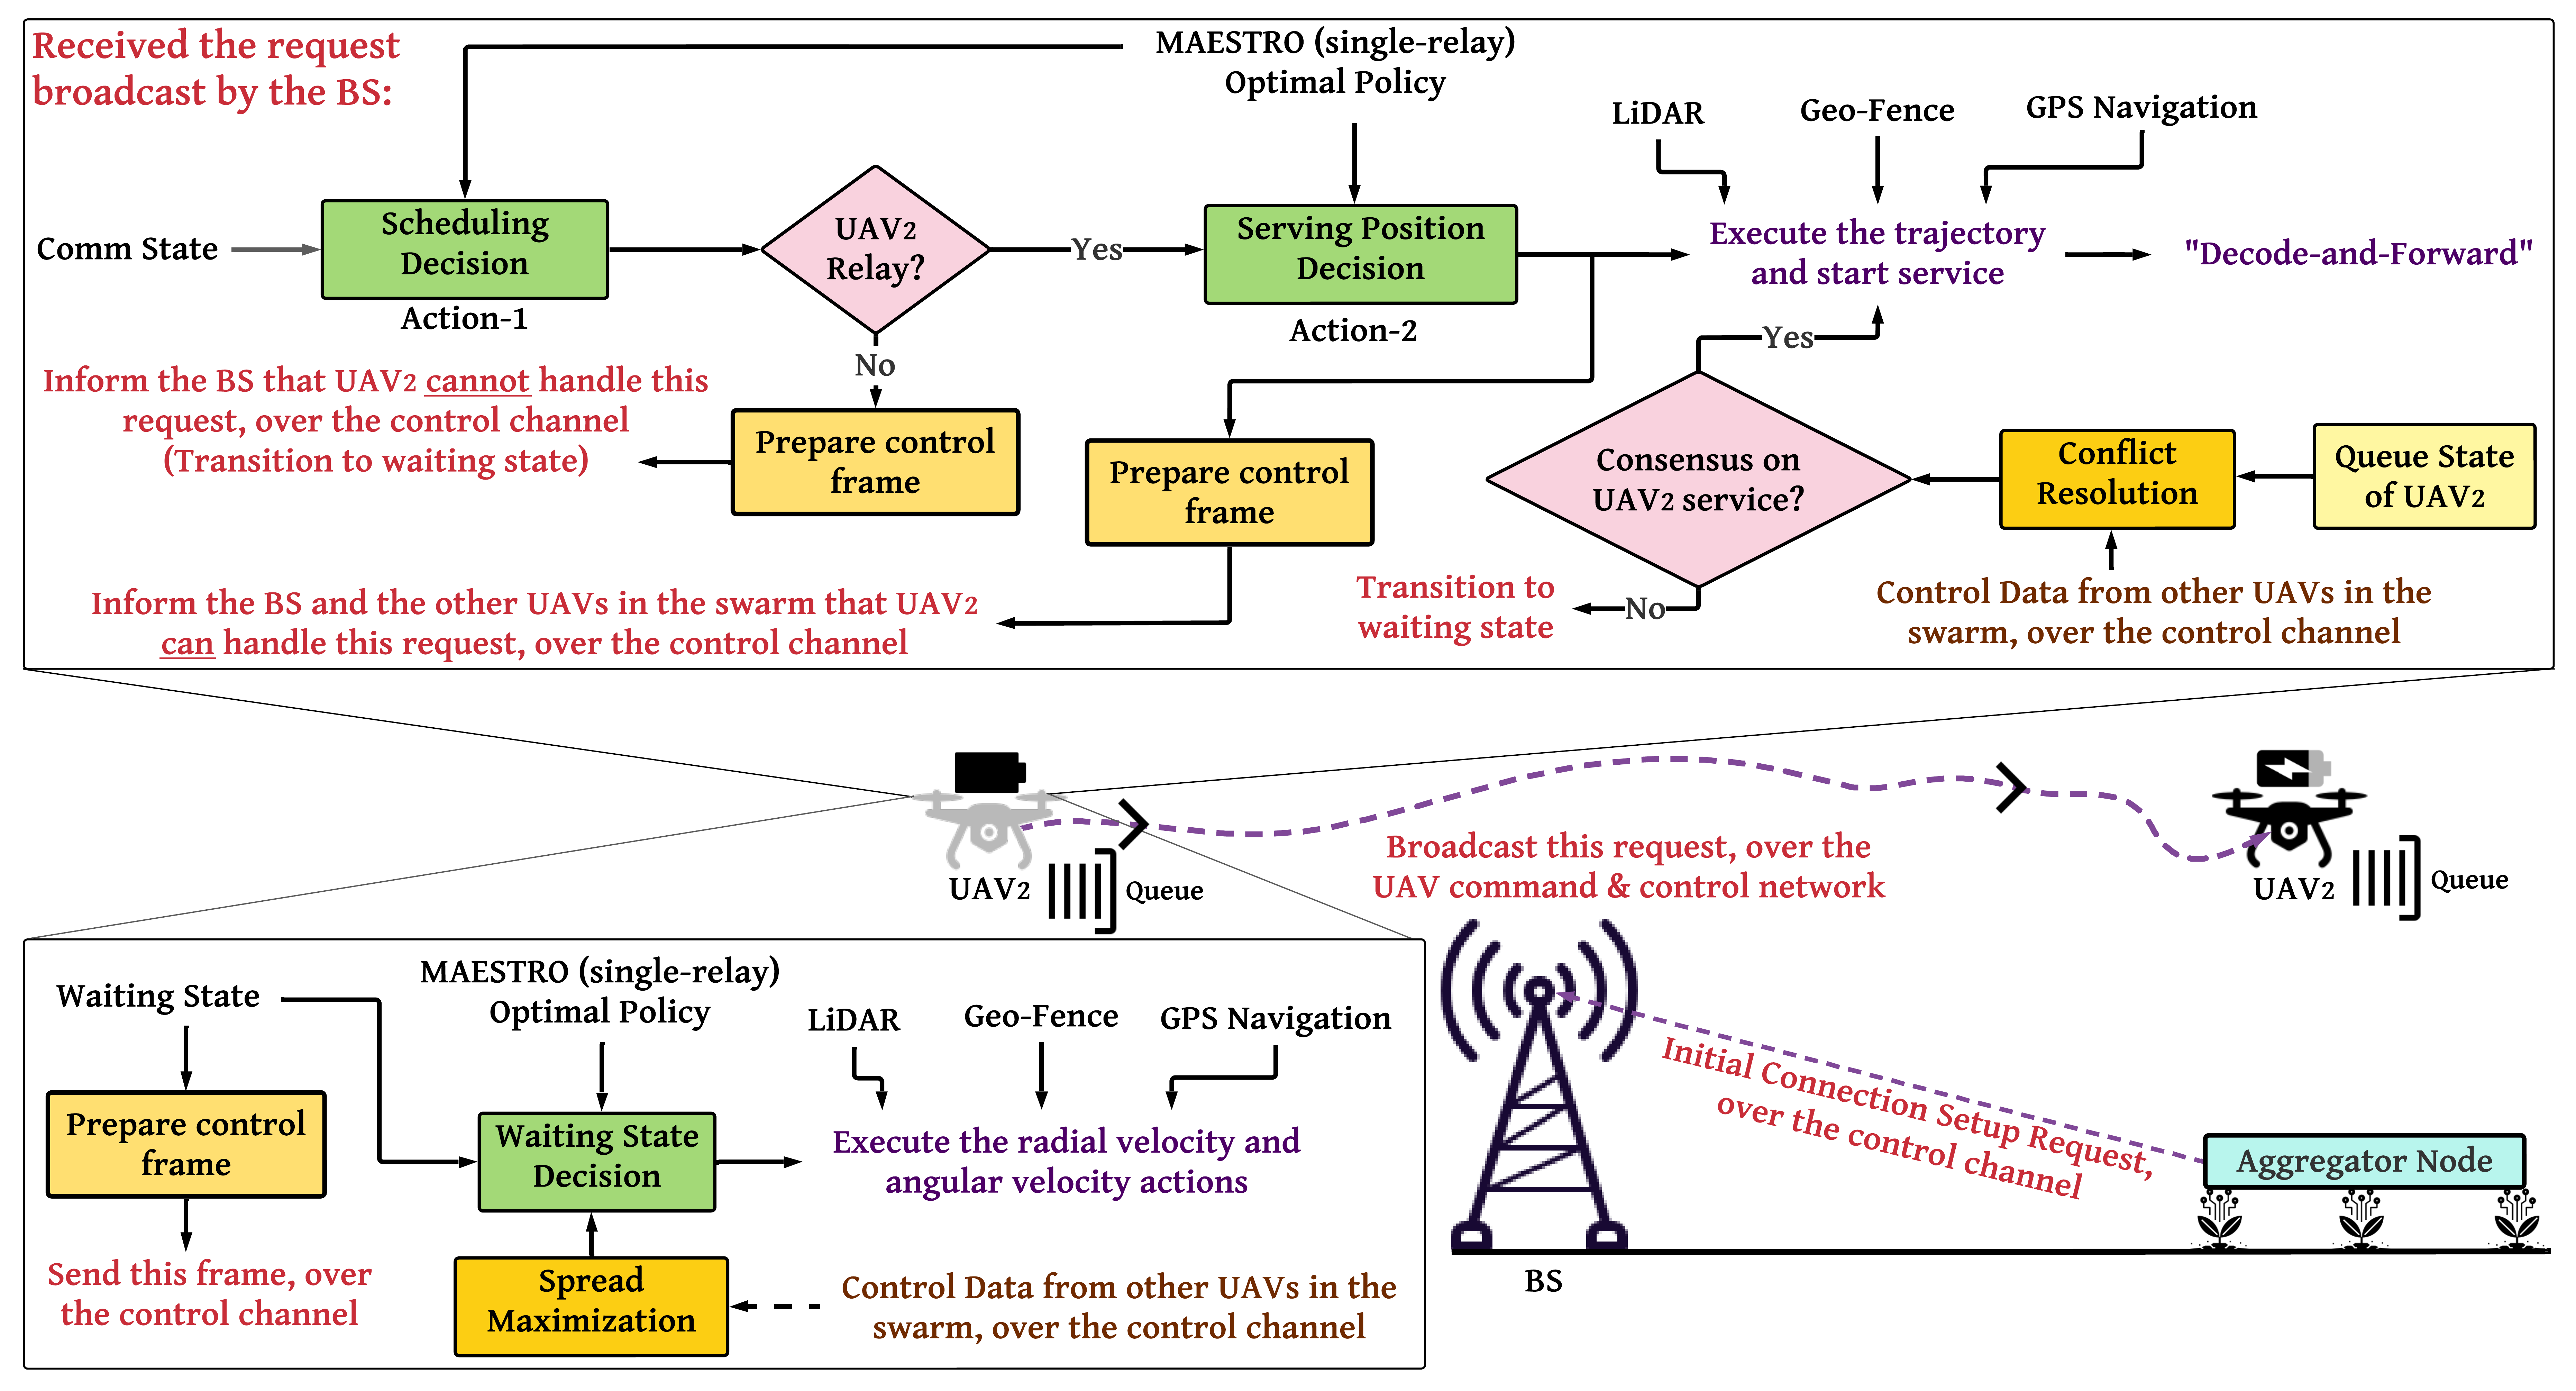
\includegraphics[width=0.9\linewidth]{figs/Sequence_of_Operations.png}
    \vspace{-2mm}
    \caption{The study of a wireless network augmented by a swarm of UAV relays in precision agriculture: an illustration outlining the sequence of operations under MAESTRO-X that occur at $\text{UAV}_{2}$ in the swarm.}
    \label{F5}
\end{figure}

\noindent{\textbf{Spread Maximization}}:
We motivate the need for spread maximization by noting that the outer action of MAESTRO's optimal waiting policy constitutes the UAV radial velocity component, which is symmetric with respect to the clockwise and counter-clockwise angular movements of the UAV. In multi-UAV settings, we can leverage this symmetry to efficiently prime and position the idle UAVs for potential new relay requests originating in the cell, which is the objective of our spread maximization algorithm. Under this context, a UAV in the swarm, waiting in a particular radius level with the optimal radial velocity action, and with the magnitude of its angular motion obtained from the optimal inner decision at this radius level \eqref{eq:MinLWP}, determines the direction of this angular motion (clockwise or counter-clockwise) based on our spread maximization heuristic---wherein each UAV relay in the {waiting} state, executes either positive (counter-clockwise) or negative (clockwise) angular movements in order to maximize the minimum distance among them. These coordinated movements among the UAVs in the swarm are made possible through periodic exchanges of control messages, whose frame structure is illustrated in Fig. \ref{F5.5}. 

With periodic exchanges of control frames (synchronized reporting period $\delta{>}0$, small), UAV $i$ waiting in the radius level $r$ with optimal radial velocity $v_{r}^{*}$ and optimal angular velocity magnitude $\theta_{c}^{*}$, parses the state flag and GPS event fields in the received control frames, and constructs a local peer list $\mathcal{L}$ of other UAVs in the waiting state. Let the current angular position of UAV $i$ be $\theta_{i}{\in}[0, 2\pi)$. First, UAV $i$ determines the index of its closest peer (in the angular dimension), i.e., $j^{*}{=}\argmin_{j{\in}\mathcal{L}}|\theta_{i}{-}\theta_{j}|$. Let the current angular coordinate of this UAV $j^{*}$ be $\theta_{j^{*}}{\in}[0,2\pi)$. Next, UAV $i$ determines its direction of angular motion as $\rho^{*}{=}\argmax_{\rho{\in}\{{+}1,{-}1\}} \left|[\theta_{i}{+}\delta\rho\theta_{c}^{*}]^{[0,2\pi)}{-}\theta_{j^{*}}\right|$, wherein UAV $i$ is moving away from its closest UAV in an attempt to spread out such that it is suitably positioned for potential new requests from this region of the cell. Then, UAV $i$ executes this angular motion until new control frames (containing updated positions) are received from its peers (at the end of the synchronized reporting period) or upon reception of a new uplink transmission request from a GN in the cell, after which it transitions to the communication state and the consensus-driven conflict-resolution process (which is discussed next) begins.

\begin{figure} [t]
    \centering
    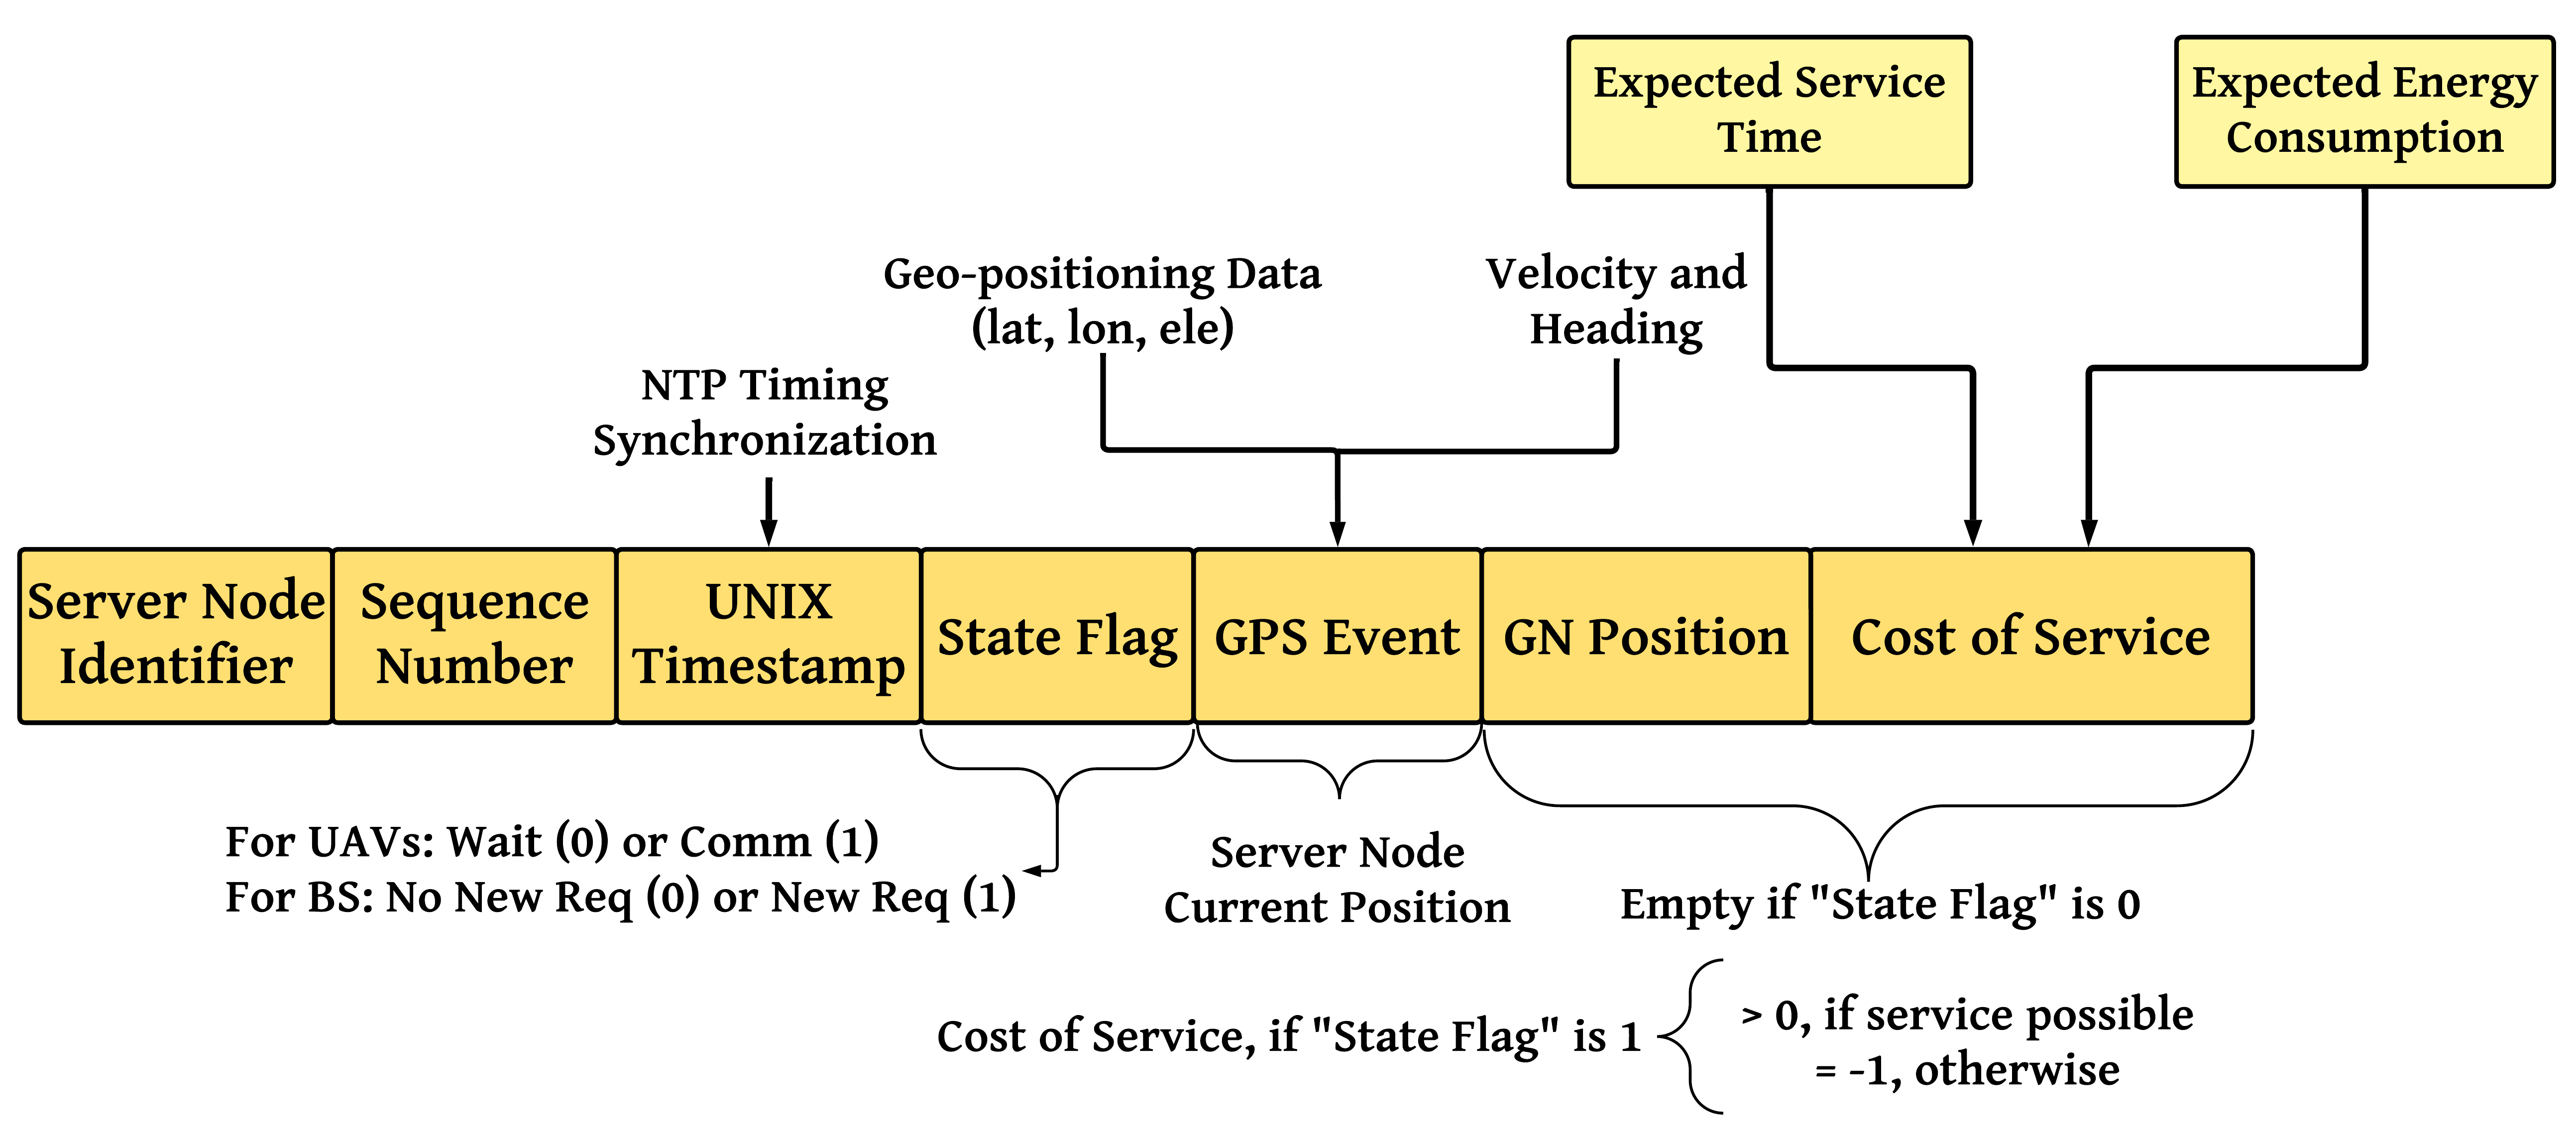
\includegraphics[width=0.9\linewidth]{figs/Control_Frame_Design.png}
    \vspace{-2mm}
    \caption{The structure of a control frame for inter-UAV and BS-UAV coordination in MAESTRO-X.}
    \label{F5.5}
\end{figure}

\noindent{\textbf{Consensus-driven Conflict Resolution}}: 
In our single-relay formulation discussed in Sec. \ref{A3}, the scheduling action involved a comparison between the Lagrangian cost of direct transmission to the BS and that of relayed service through the UAV. However, while extending to UAV swarms via policy replication and with the incorporation of queuing dynamics, this single-agent scheduling decision has to be enhanced to 1) resolve conflicts among server nodes (BS and UAVs), when two or more of them decide to serve a new GN request (according to their local execution of MAESTRO) and hence facilitate a consensus on the best possible node to serve the GN; and 2) account for the queue wait times experienced by the GN at each potential server node. Accordingly, the single-agent comparison operation for scheduling is scaled to multiple UAVs and modified to incorporate the impact of queuing dynamics: this augmentation is termed consensus-driven conflict resolution and is driven by a cost-of-service metric defined below. 

For a request at $(r,\theta)$, $\frac{L}{\bar{R}_{GB}(r)}{+}t_{Q|\text{BS}}$ at the BS and $\tilde{f}(\mathbf{p}_{i}^{*},\mathbf{v}_{i}^{*}){=}\hat{f}(\mathbf{p}_{i}^{*},\mathbf{v}_{i}^{*}){+}(1{-}\nu P_{\mathrm{avg}})t_{Q|i}$ at an available UAV $i$, constitutes the comparison cost metric, where $t_{Q|\text{BS}}$ denotes the waiting time in a BS queue and $t_{Q|i}$ denotes the wait time for the request in the UAV $i$ queue. Specifically, this queue wait time includes the time needed to serve the requests already in the queue. Moreover, note that in our construction---corresponding to the Poisson arrival process and the number of orthogonal channels at the BS and the UAVs---the BS models an M/G/$N_{B}$ queuing system while the UAVs model an M/G/$1$ queue each. When a new request originates in the cell, the UAVs already serving a GN continue to do so, i.e., they do no participate in the consensus-driven conflict resolution process. On the other hand, UAVs in the {waiting} states transition into their respective {communication} states: let these UAVs constitute the set $\mathcal{L}'$. The BS along with these relays are deemed to be available. These available server nodes exchange collaboration messages over the command-and-control network (see Fig. \ref{F5.5}). These messages comprise the cost-of-service metric $\tilde{f}(\mathbf{p}_{i}^{*},\mathbf{v}_{i}^{*})$ which enables the available nodes to arrive at a consensus on the best choice to serve the request, i.e., if $\frac{L}{\bar{R}_{GB}(r)}{+}t_{Q|\text{BS}}{<}\tilde{f}(\mathbf{p}_{i}^{*},\mathbf{v}_{i}^{*}),{\forall}i{\in}\mathcal{L}'$, then direct transmission to the BS is scheduled; else, the GN request is relayed through UAV $i^{*}{=}\argmin_{i{\in}\mathcal{L}'}\tilde{f}(\mathbf{p}_{i}^{*},\mathbf{v}_{i}^{*})$.
\vspace{-4mm}


\section{Simulation Setup and Numerical Evaluations}\label{S6}
\vspace{-2mm}

In our numerical evaluations, we use a channel bandwidth of $B=$ \qty[mode=text]{5}{\mega\hertz}; for all links, NLoS attenuation constant $\kappa=$ \qty[mode=text]{0.2}{}, $1$-meter reference SNR $\frac{\beta_{0}P}{\sigma^{2}\Gamma}=$ \qty[mode=text]{40}{\decibel}, LoS path-loss exponent $\alpha=$ \qty[mode=text]{2}{}, NLoS path-loss exponent $\tilde{\alpha}=$ \qty[mode=text]{2.8}{}, Rician $K$-factor parameters $k_{1}=$ \qty[mode=text]{1}{} and $k_{2}=$ \qty[mode=text]{0.05}{} \cite{Rician}, and LoS probability parameters $z_{1}=$ \qty[mode=text]{9.61}{} and $z_{2}=$ \qty[mode=text]{0.16}{} \cite{OptimalAltitude}; UAV height $H_{U}=$\qty[mode=text]{200}{\meter}; BS antenna height $H_{B}=$\qty[mode=text]{80}{\meter}; maximum UAV velocity $V_{\mathrm{max}}=$ \qty[mode=text]{55}{\meter\per\second}; and cell radius $a=$ \qty[mode=text]{1000}{\meter}. The UAV power consumption model uses the relationship and parameters detailed in \cite{SCA}. To solve \eqref{eq:PolDecomp}, we discretize the state and action spaces and apply linearly-interpolated value iteration. We discretize the states with $N_{\mathrm{sp}}=$ \qty[mode=text]{25}{} equispaced radii values, with $12$ GNs in each level; and $R_{\mathrm{sp}}=$ \qty[mode=text]{25}{} equispaced radial velocity actions for $v_r{\in}\{-V_{\mathrm{max}},{\dots},V_{\mathrm{max}}\}$. Lastly, $\Delta_{0}$ is chosen to satisfy $e^{-\Lambda'\Delta_{0}}{=}$ \qty[mode=text]{0.93}{}, such that it is unlikely to receive two or more GN requests in $\Delta_{0}$.

\begin{figure} [t]
      \begin{subfigure}{0.5\linewidth}
	     \centering
         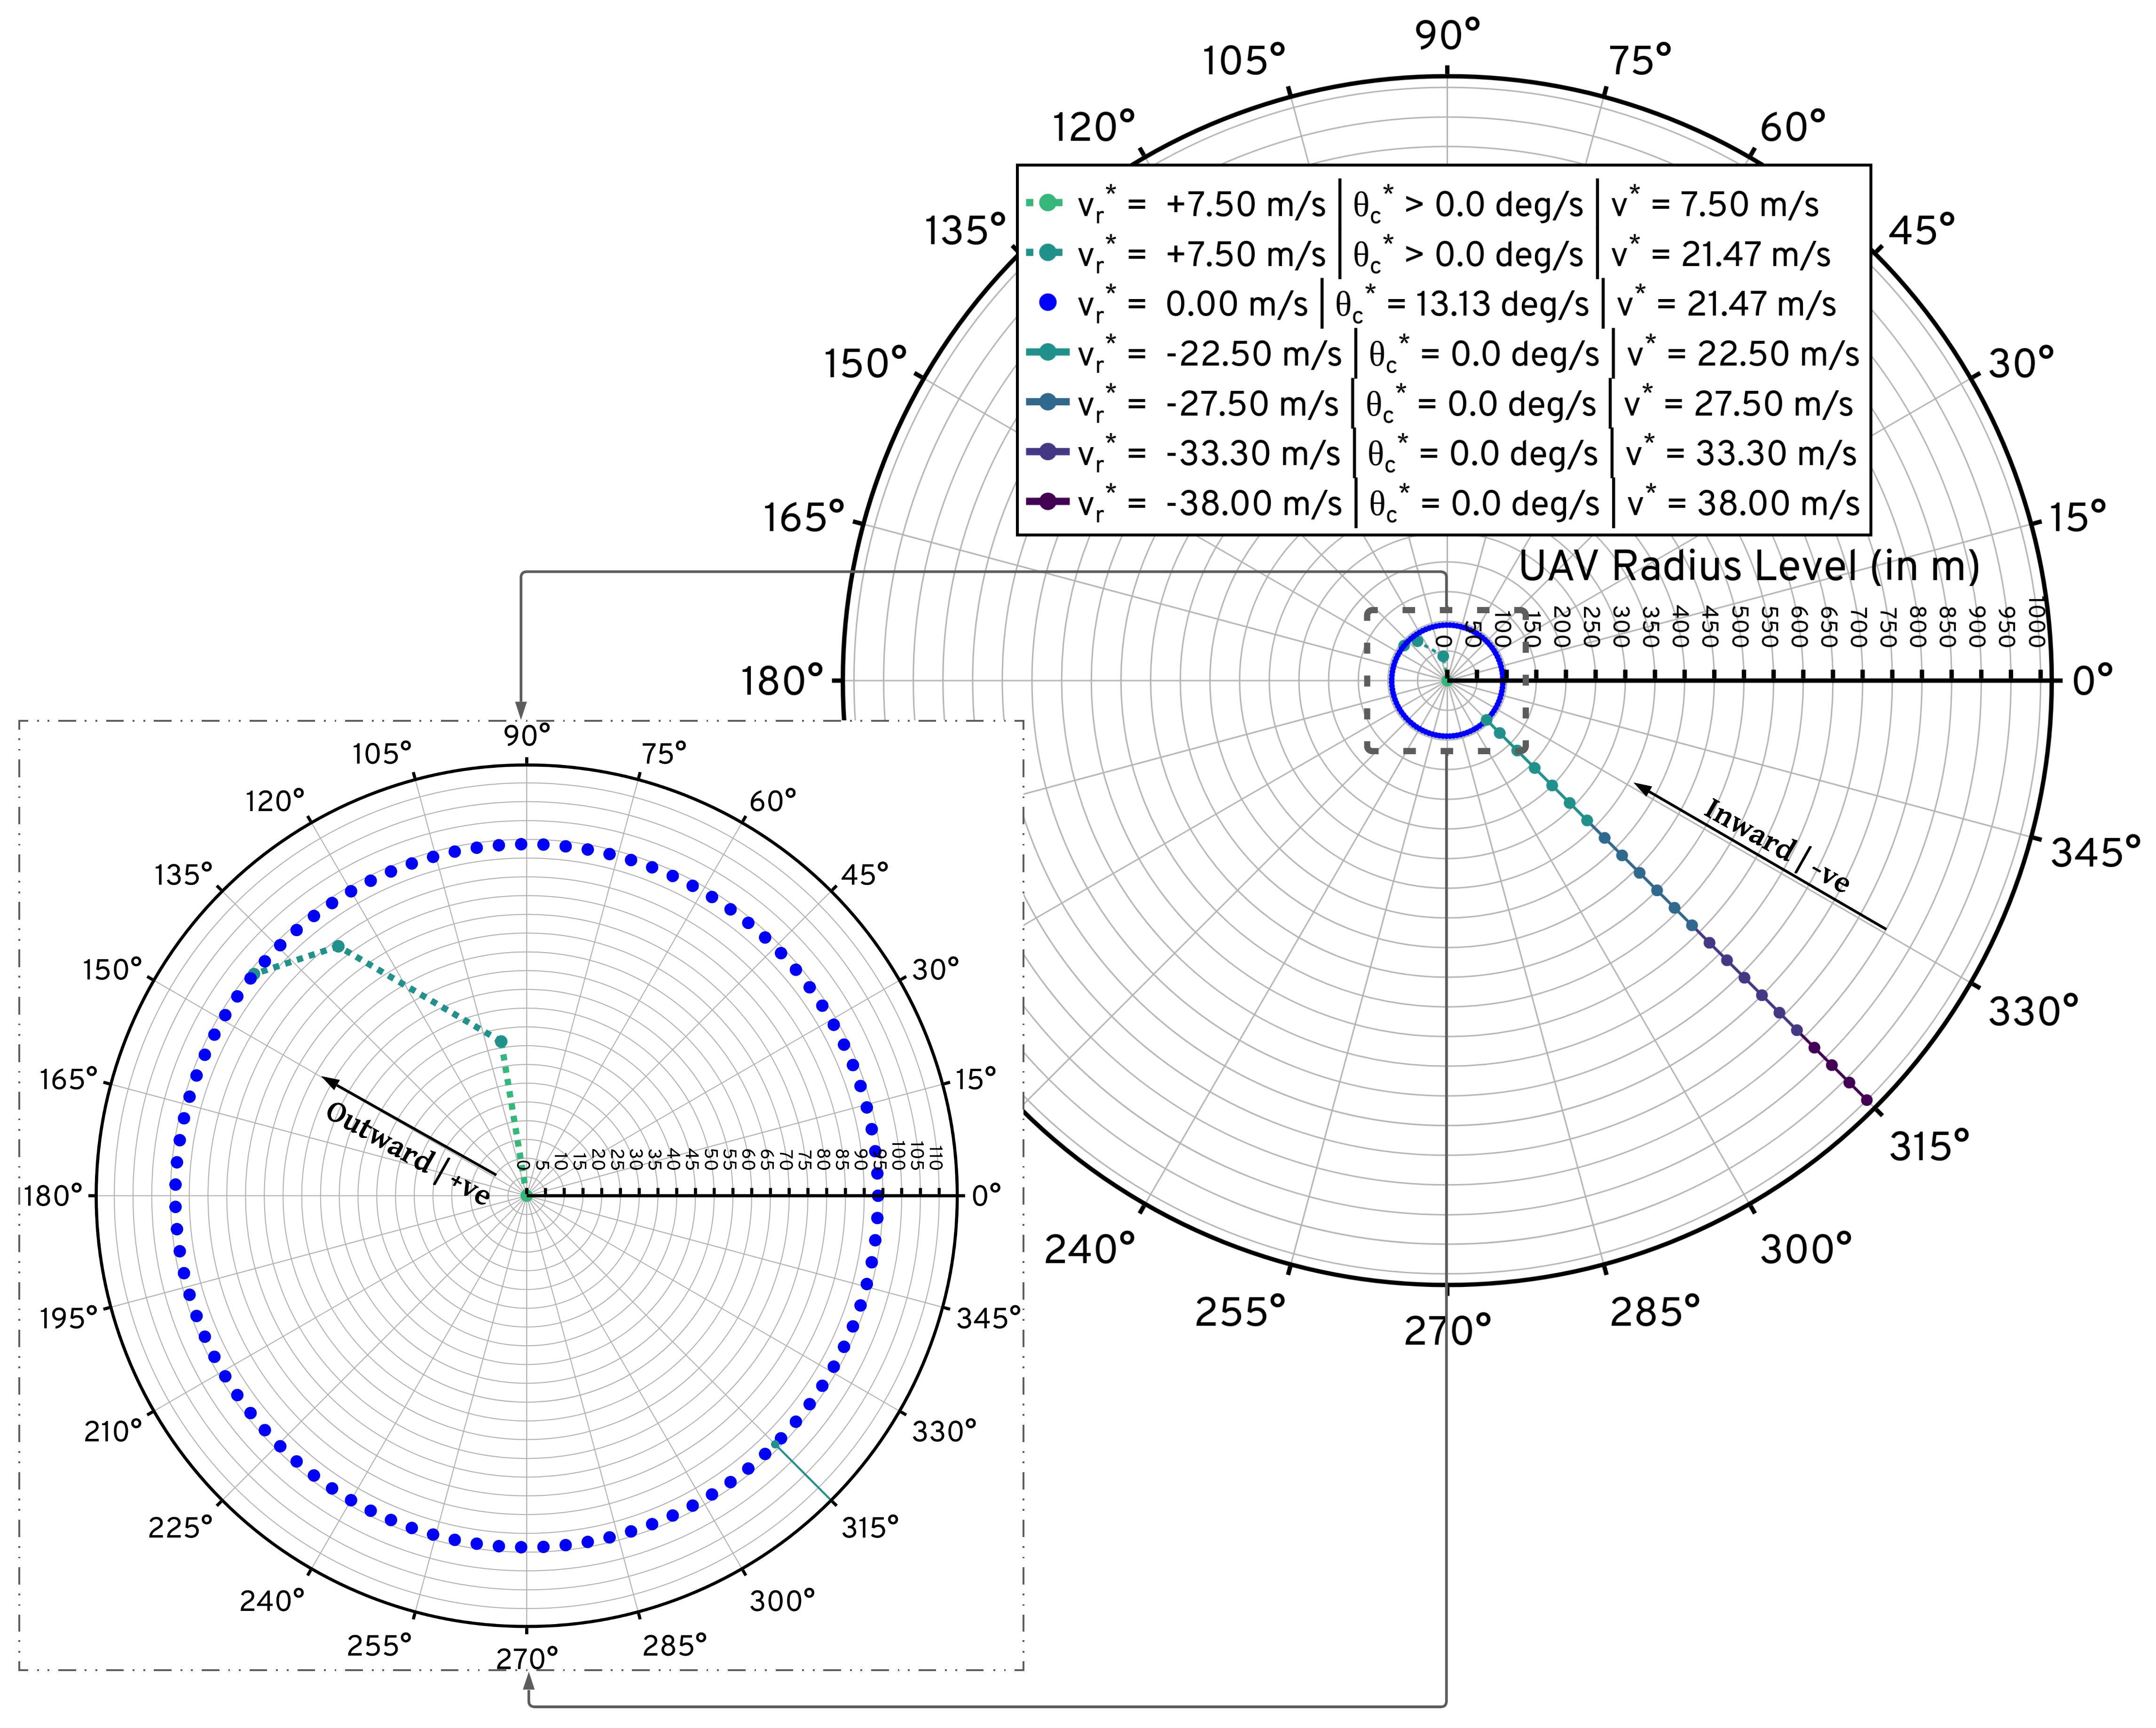
\includegraphics[width=0.9\linewidth]{figs/Optimal_Waiting_Policy_1Mb.png}
         \caption{Optimal Wait Policy for $L{=}1$ Mb}
		 \label{F6}
	 \end{subfigure}
     \begin{subfigure}{0.516\linewidth}
         \centering
  		 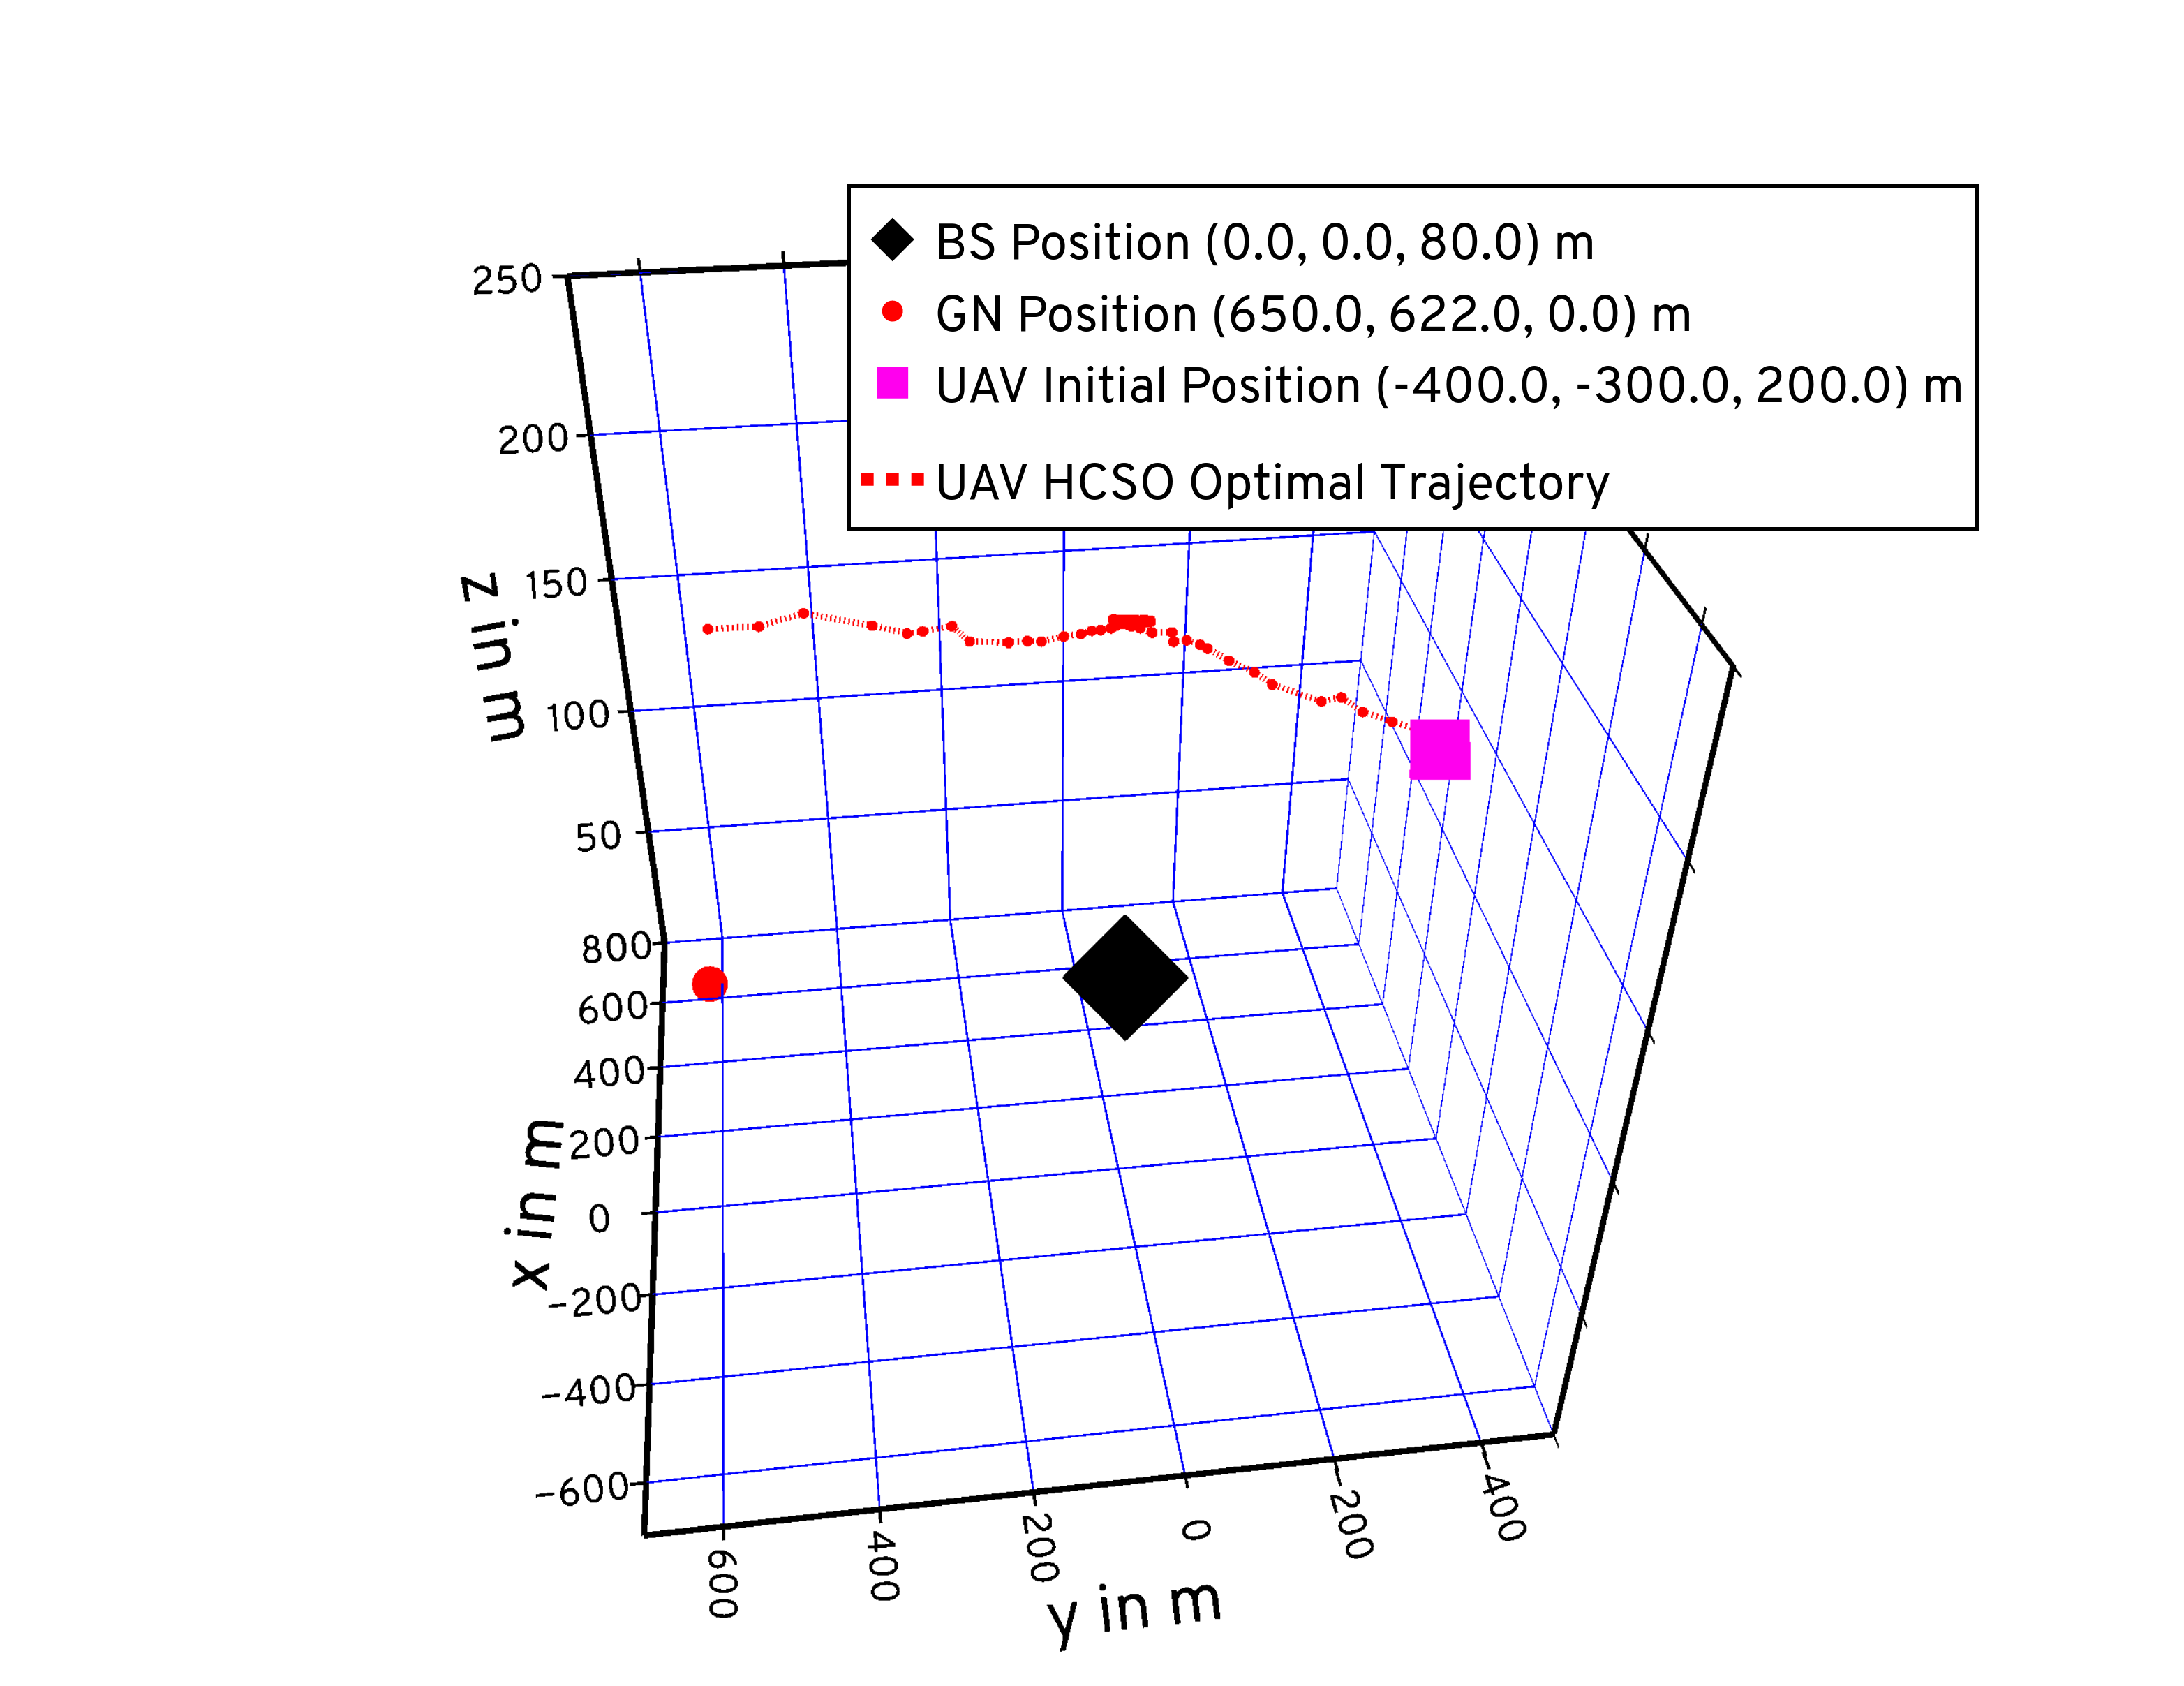
\includegraphics[width=0.9\linewidth]{figs/Optimal_UAV_Trajectory.png}
		 \caption{Optimal trajectory simulation for $L{=}10$ Mb}
         \label{F7}
     \end{subfigure}
     \vspace{-2mm}
     \caption{(a) The execution of the optimal waiting state policy at a UAV for $L{=}1$ Mb with $P_{\mathrm{avg}}{=}1.2$ kW; (b) The optimal trajectory simulation of $\text{UAV}_{2}$ under the MAESTRO-X framework for $L{=}10$ Mb and $P_{\text{avg}}{=}1.2$ kW.}
\end{figure}

First, to analyze the optimal waiting behavior of a UAV relay in our control framework, we fix $P_{\mathrm{avg}}{=}1.2$ kW and $L{=}1$ Mb. Fig. \ref{F6} shows that the UAV moves to and waits ($v_{r}^{*}{=}0$) by flying around an optimal radius level ($r_{0}^{*}{\approx}95$ m) to address two considerations: to be well-positioned for future requests and to fly at the power-minimizing velocity so as to reduce its energy consumption. Moreover, angular velocity optimization adheres to the observations in \cite{SCA} about optimizing towards $P_{\mathrm{min}}$ (corresponding to $V{=}$ \qty[mode=text]{22}{\meter\per\second}). Next, Fig. \ref{F7} depicts a simulated execution of the optimal trajectory of UAV$_{2}$ (obtained via HCSO in Sec. \ref{S4}) under $L{=}10$ Mb traffic payloads and an average power constraint of $P_{\text{avg}}{=}1.2$ kW, when an active GN request at $(650,622,0)$ in the cell is scheduled to be served by the UAV---via the D\&F protocol detailed in Sec. \ref{A3}---with this trajectory beginning at the initial UAV position of $(-400,-300,200)$.

Second, we evaluate the delay-power trade-off of MAESTRO-X and compare with with state-of-the-art algorithms: Successive Convex Approximation (SCA) \cite{SCA}, Constrained SCA with Alternating Direction Method-of-Multipliers (CSCA-ADMM) \cite{CSCA-ADMM}, and Double Deep Q-Networks with Combined Experiential Replay (DDQN-CER) \cite{DDQN}. As depicted in Figs. \ref{F8} and \ref{F9}, for uplink transmission requests of size $L{=}1$ Mb from the $300$ GNs in the cell, we observe the following improvements in performance over custom network deployment heuristics and state-of-the-art frameworks, averaged over $10,000$ requests with a Poisson arrival rate of $1$ request every $60$ s. Considering only direct transmissions to a $10$-channel OFDMA BS at the cell center, we find a significant reduction in the average communication delay experienced by the GNs in the cell, by employing UAVs to relay data traffic. Also, we observe that employing dynamic UAVs with optimized trajectories demonstrate lower service delays compared to static relay deployments---specifically, for a swarm of $3$ UAV relays, with $L{=}1$ Mb and a per-UAV power consumption of $1.37$ kW, our solution services GN requests $12.5{\times}$ faster than a static deployment of $3$ UAVs positioned equidistant from the cell center. With CVXPY implementations of joint multi-agent SCA strategies \cite{SCA, CSCA-ADMM}, we note that our control system with $1$ UAV relay exceeds the QoS performance offered by $3$ relays under these SCA approaches. Also, at $P_{\text{avg}}{=}1.1$ kW, MAESTRO-X demonstrates $3.25{\times}$ faster service times relative to the DDQN solution in \cite{DDQN}. 

Additionally, Fig. \ref{F9} illustrates the components of QoS latencies experienced by GNs in our network: the transmission delay (in green) which constitutes the execution of either direct-BS transmission or the D\&F protocol of relayed-service through a UAV, and the amount of time spent waiting (in red) in one of $N_{B}{=}10$ BS queues or a UAV queue. Expectedly, under a Join-Fastest-Queue heuristic, the BS-only M/G/$N_{B}$ queuing system encounters zero queue wait times due to the availability of multiple queues; similar trends are observed across UAV-assisted implementations when the number of UAVs in the swarm increases. Moreover, we observe a direct correlation between the transmission times and the queue wait times, i.e., for $1$-UAV networks with high transmission times (e.g., static UAVs, SCA \cite{SCA}, DDQN-CER \cite{DDQN}), requests experience long delays waiting to be picked up by this single UAV queue under relayed-service. 

\begin{figure} [t]
     \begin{subfigure}{0.53\linewidth}
         \centering
         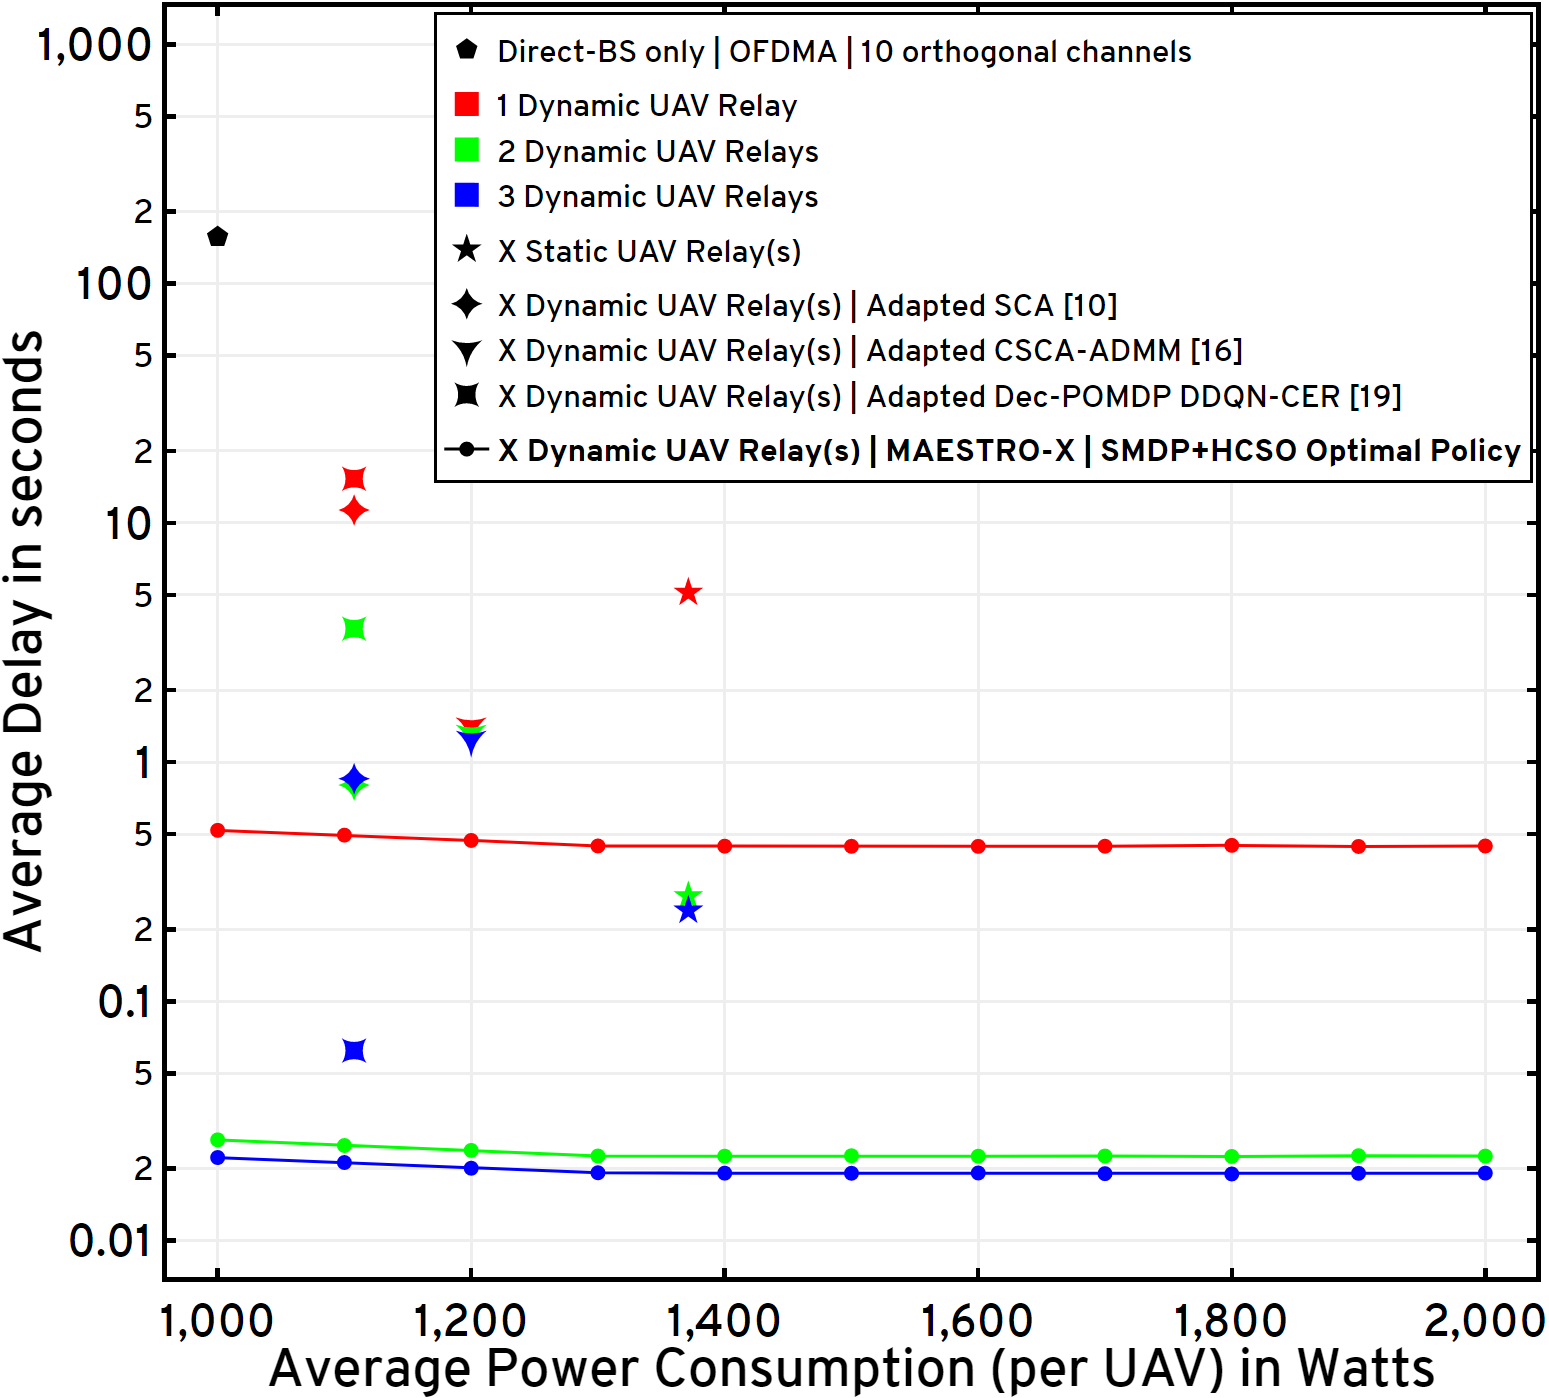
\includegraphics[width=0.9\linewidth]{figs/Delay_Power_Tradeoff_1Mb.png}
         \caption{Delay-Power Trade-off}
         \label{F8}
     \end{subfigure}
     \begin{subfigure}{0.47\linewidth}
         \centering
         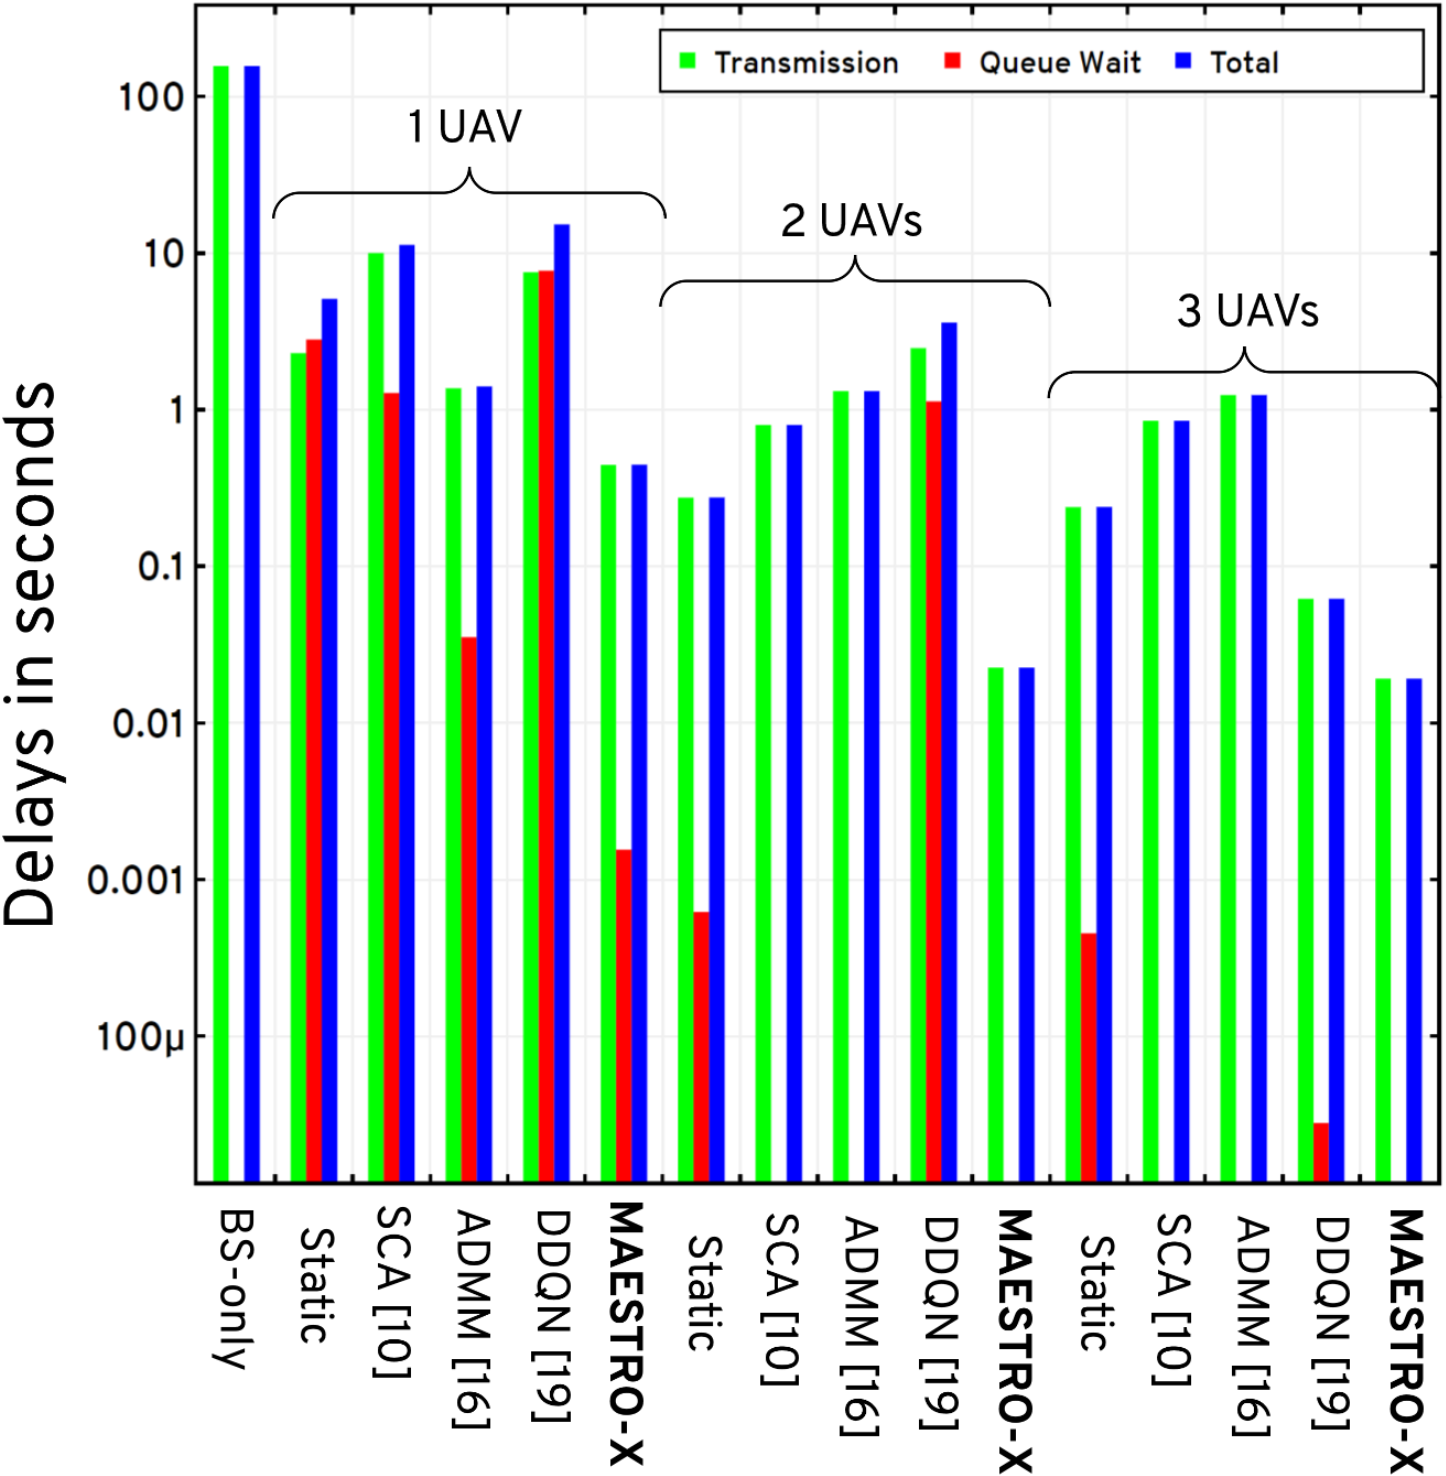
\includegraphics[width=0.9\linewidth]{figs/Delay_Power_Histogram_1Mb.png}
         \caption{Delay-Power Histogram}
         \label{F9}
     \end{subfigure}
     \vspace{-2mm}
     \caption{The traces (a) and histogram (b) constituting the average service latencies versus the average power constraint for MAESTRO-X under $L{=}1$ Mb: Comparisons with custom deployment heuristics and with the state-of-the-art.}
\end{figure}

Third, as shown in Fig. \ref{F10}, bench-marking our MAESTRO-X framework against both model-based \cite{CSCA-ADMM} and model-free \cite{DDQN} solutions in the state-of-the-art, we observe that the decoupled policy replication across the swarm---with suitable supplementary heuristics---ensures that our solution constitutes a practically feasible formulation even with higher-degrees of scaling in the number of UAVs in the swarm. The CSCA-ADMM approach in \cite{CSCA-ADMM} and the DDQN-CER approach in \cite{DDQN} involve prohibitively large policy convergence times when the number of the UAVs in the swarm is scaled beyond $N_{U}{=}5$ and $N_{U}{=}6$, respectively. All implementations are in Python, and this bench-marking is performed on a compute node with $2{\times}$ $64$-core AMD EPYC Milan 7763 CPUs, $16{\times}$ $64$ GB DDR$4$ memory, and $4{\times}$ NVIDIA A$100$ GPUs with $40$ GB VRAM each. The CSCA-ADMM solution in \cite{CSCA-ADMM} suffers poor bench-marking performance relative to MAESTRO-X due to a joint multi-UAV construction involved in its CVXPY-SCS implementation; the DDQN-CER solution in \cite{DDQN} involves larger policy convergence times due to an underlying model-free formulation that employs combined MDP state and action spaces.

\begin{figure}[t]
	\begin{subfigure}{0.494\linewidth}
  		\centering
  		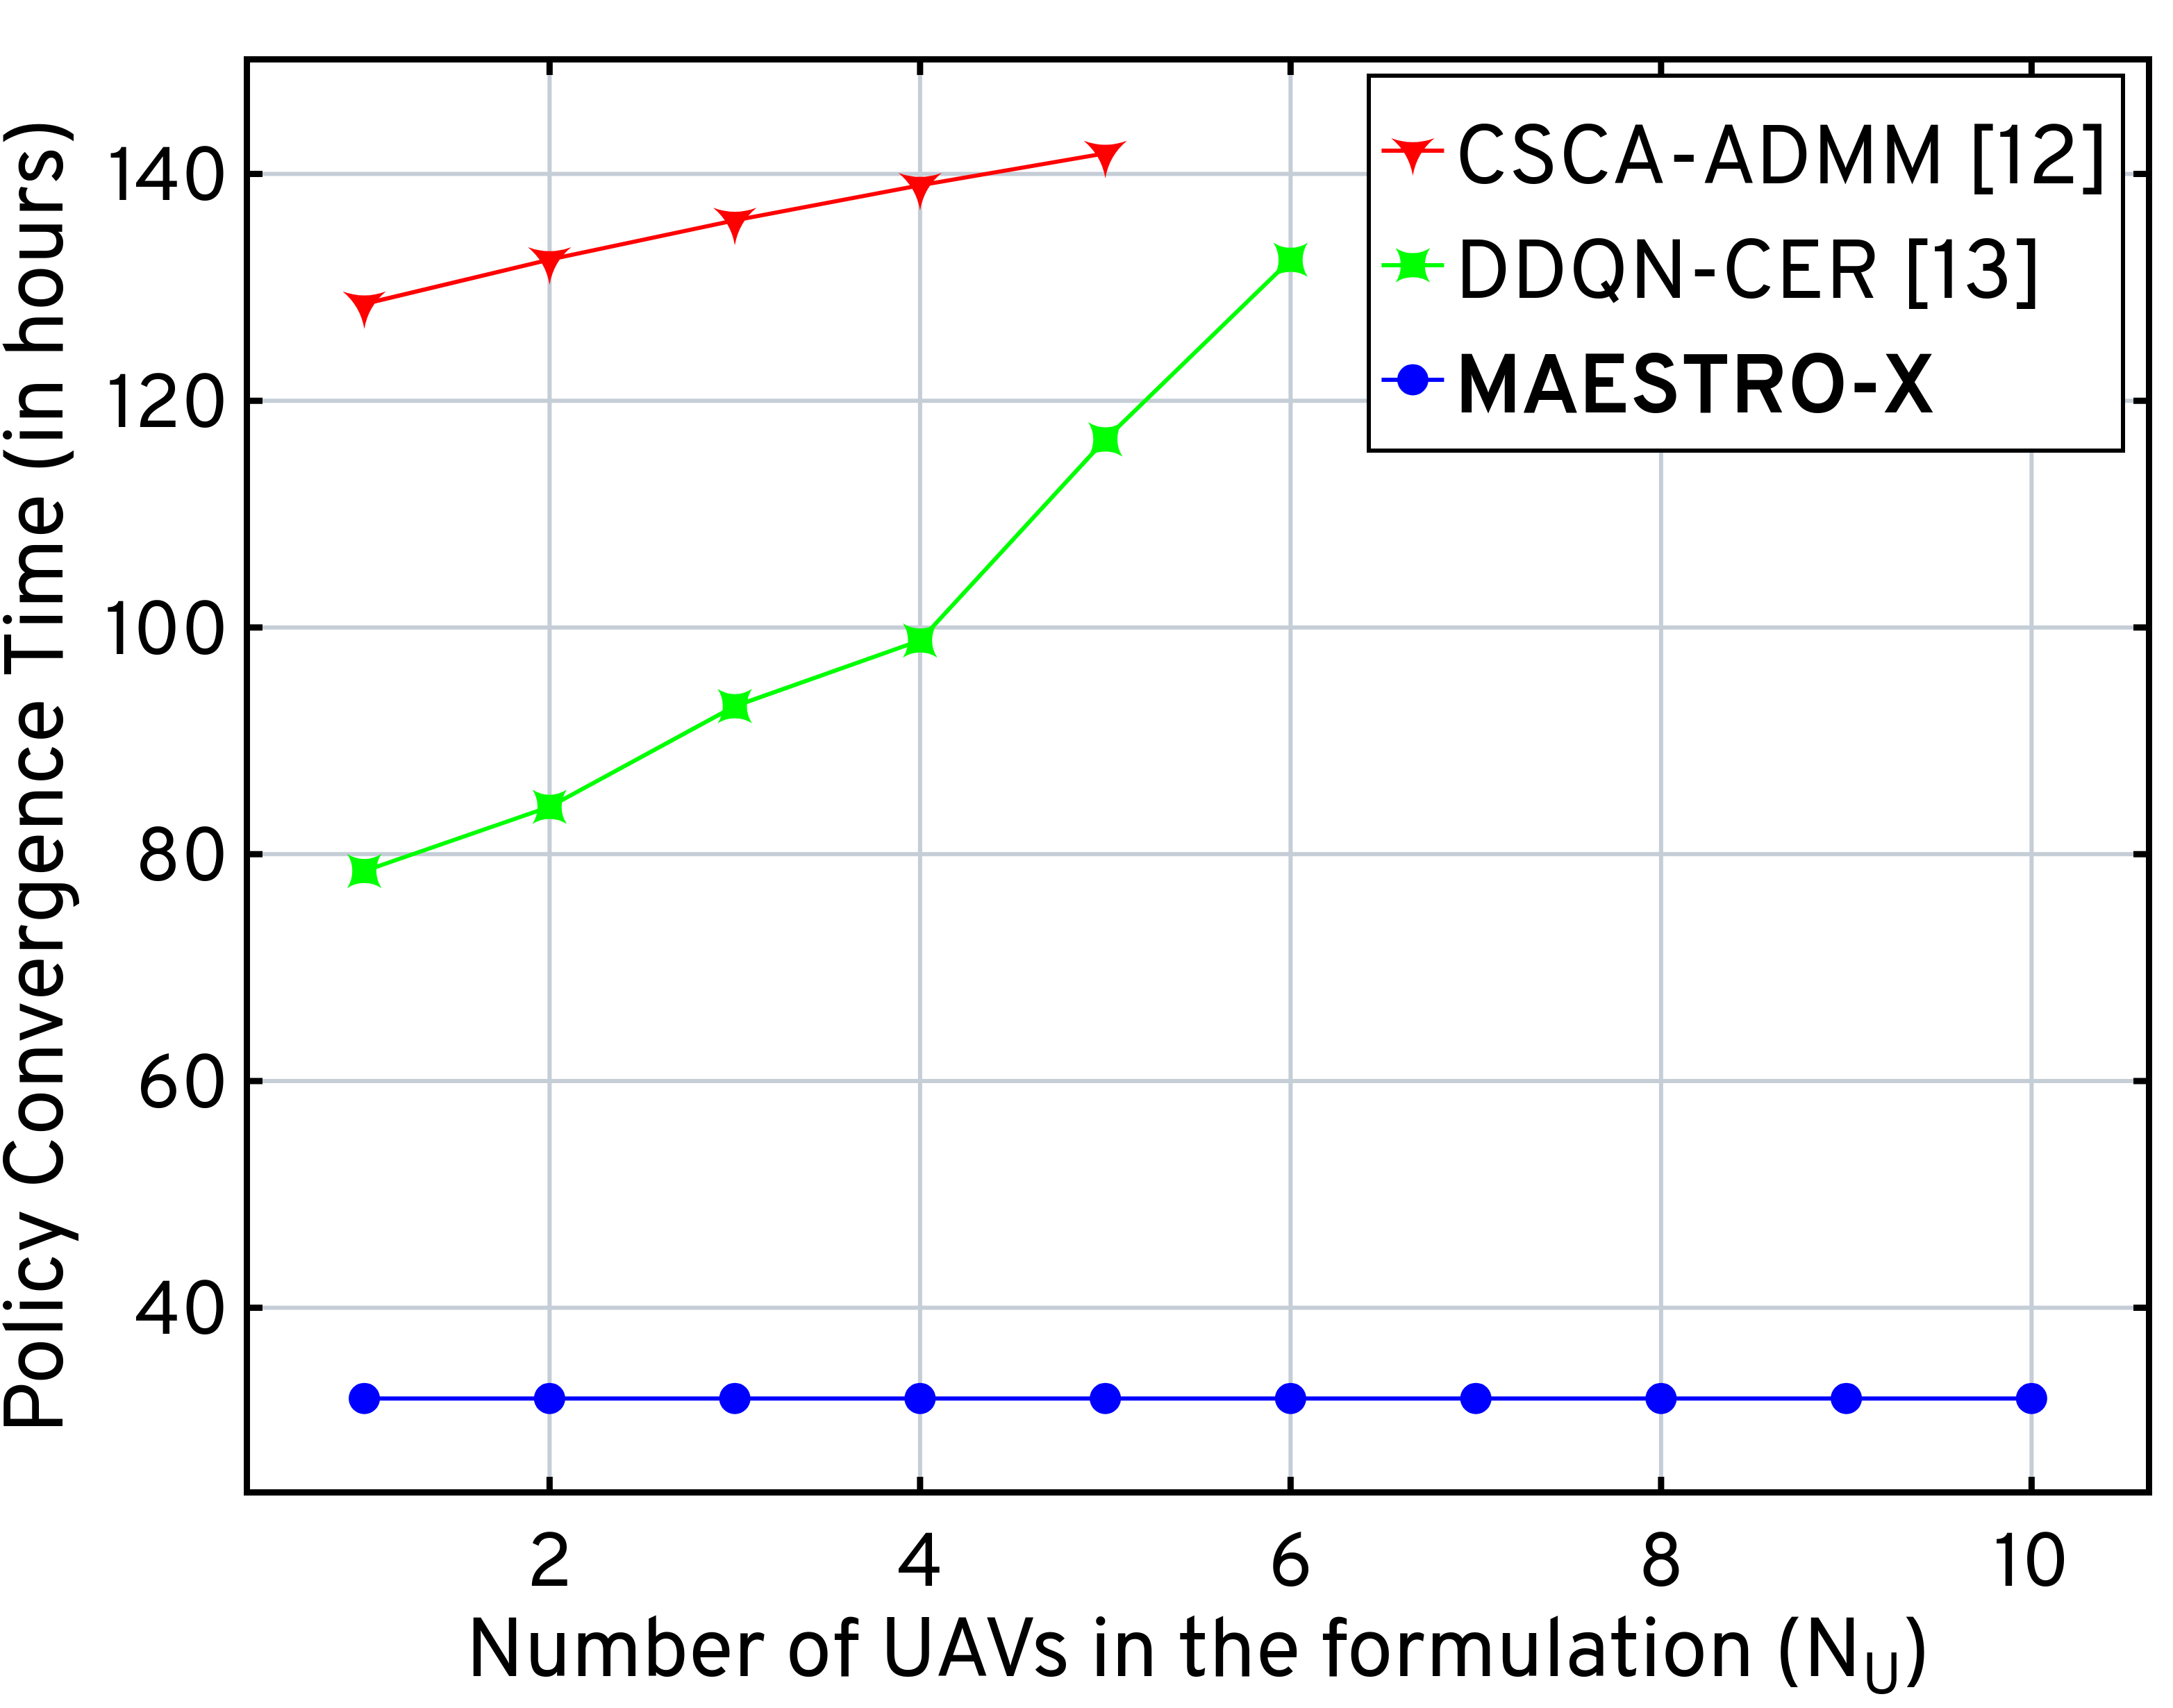
\includegraphics[width=0.9\linewidth]{figs/Computational_Complexity.png}
  		\caption{Computation Time Bench-marking}
  		\label{F10}
	\end{subfigure}
	\begin{subfigure}{0.506\linewidth}
         \centering
         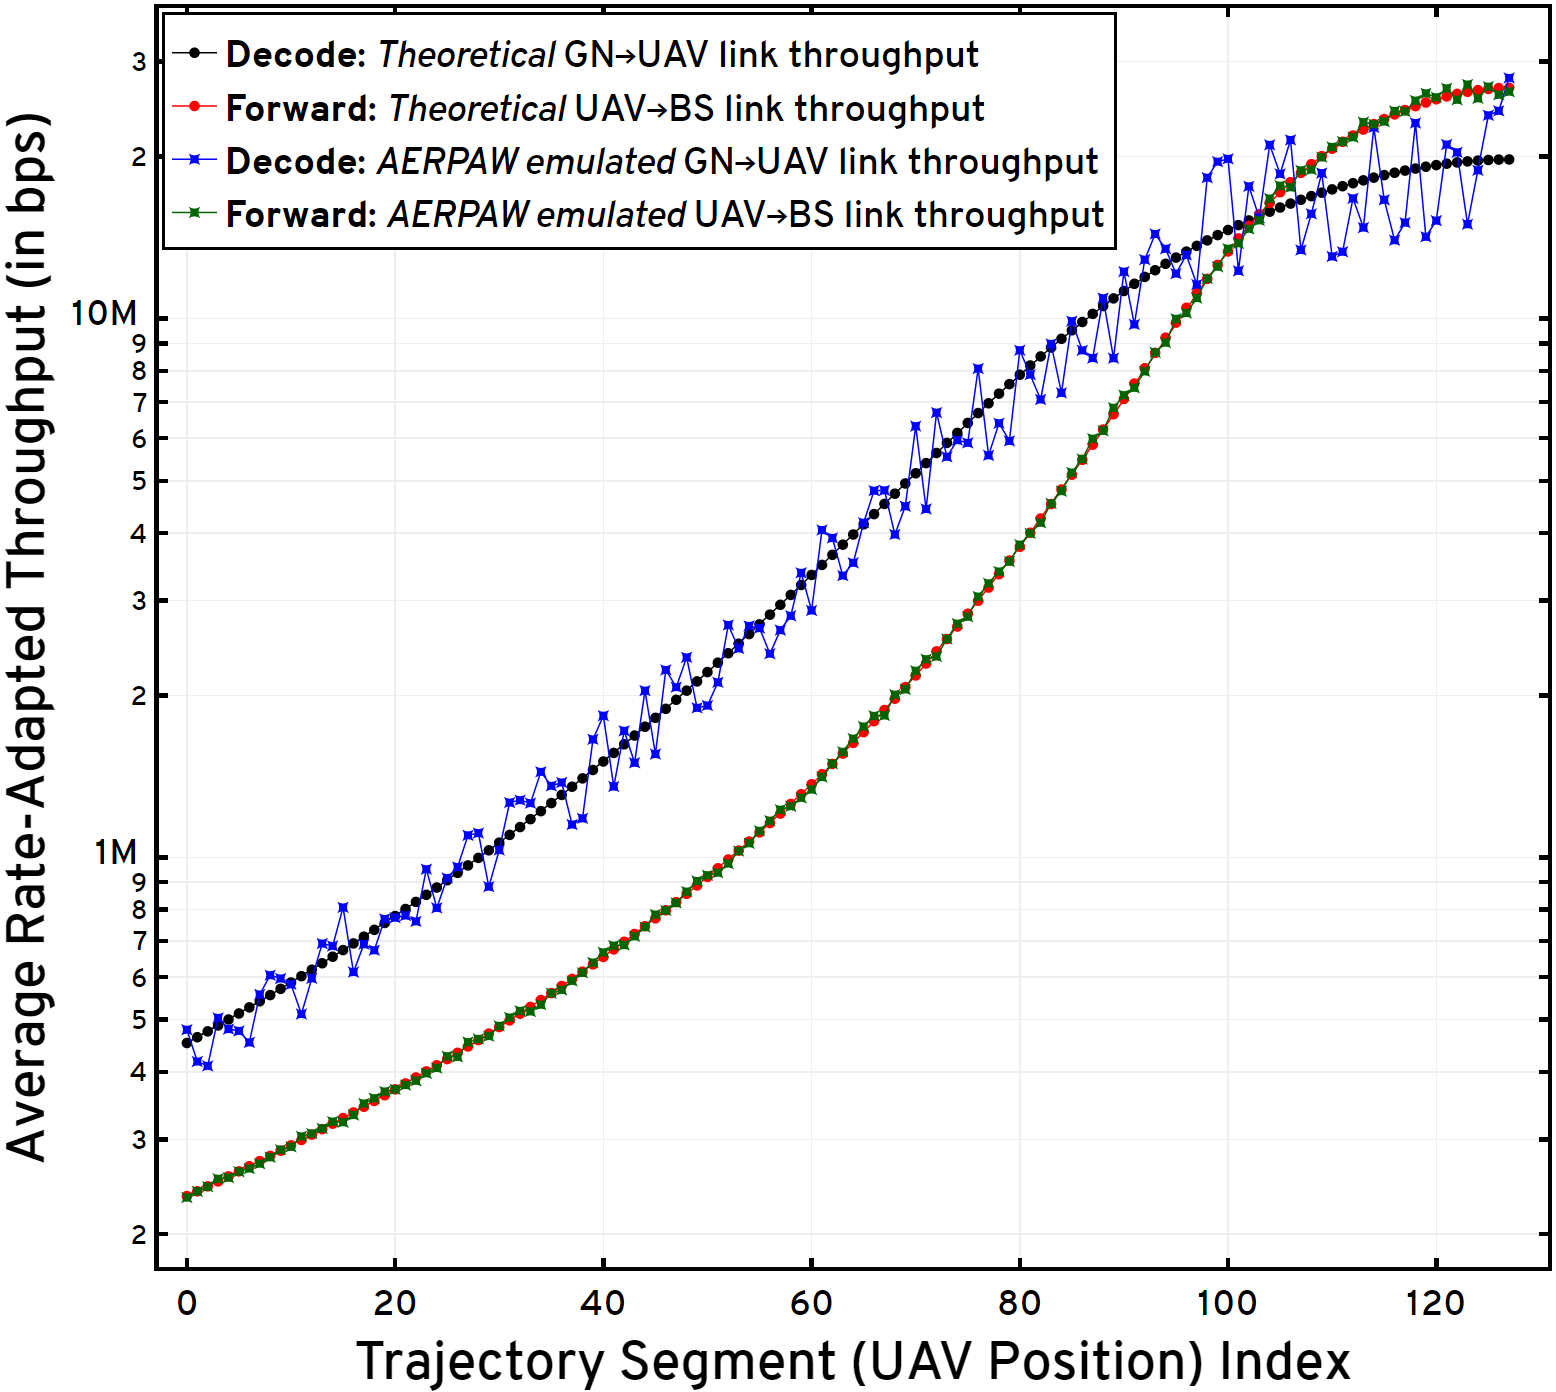
\includegraphics[width=0.9\linewidth]{figs/AERPAW_Emulated_Throughput_Comparisons.png}
         \caption{Theoretical vs AERPAW Emulated Throughput}
         \label{F11}
     \end{subfigure}
	\vspace{-2mm}
	\caption{(a) Computational bench-marking of MAESTRO-X against relevant frameworks in the state-of-the-art; (b) Comparisons between the theoretical rate-adapted throughput achieved in our simulations and that obtained during the emulated execution of the optimal trajectory for $L{=}10$ Mb and $P_{\text{avg}}{=}1.2$ kW on NSF AERPAW.}
\end{figure}

Finally, we discuss the emulations of our optimal communication state policy on the NSF AERPAW platform: the setup of this emulation process on the advanced wireless platform includes provisioning both fixed (GN/BS) and portable node (UAV) resources, OFDM PHY at all radios equipped with adaptive modulation and coding driven by SNR feedback, and the integration of our optimal control framework with the underlying radio and vehicle control libraries. Controlled in software using GNURadio libraries, the radio nodes in our emulation include the fixed BS (at the center of the cell), the fixed GN (at a designated position within the cell), and the UAV (portable node) flying at a fixed height of $200$ m. To efficiently exploit A2G channel dynamics, at each of these radios, rate adaptation centers around an adaptive modulation and coding strategy with the instantaneous SNR fed back to determine the best modulation scheme and code rate for the transmitted symbols. We emulate the optimal service trajectory of the UAV shown in Fig. \ref{F7}, as it traverses its decode and forward paths, orchestrated from within MAESTRO-X via asynchronous remote calls using the platform-provided vehicle control libraries over the MAVLink interface: considering the same channel and mobility parameters, Fig. \ref{F11} depicts the comparison between the throughput achieved by our setup in this emulation environment against that achieved in our simulations, as the UAV traverses the $M$-segments ($M{=}256$) of the optimal trajectory to serve the request. Here, we observe that the emulated throughput closely matches the theoretical one described in \eqref{TBar}, which was derived under the idealistic assumptions of capacity achieving codes and throughput maximizing rate.
\vspace{-4mm}


\section{Conclusions}\label{S7}
\vspace{-2mm}

In this paper, we propose MAESTRO-X, a framework for the decentralized orchestration of a swarm of rotary-wing UAV relays in cellular networks, augmenting the coverage and service capabilities of a terrestrial BS. First, we specialize our system model to single-UAV deployments and design the optimal scheduling and trajectory optimization policy under an SMDP formulation (via value iteration and HCSO). Next, we extend this single-relay policy to distributed deployments of two or more UAVs by supplementing the policy with multi-UAV coordination heuristics and M/G/$x$ queuing management, and replicate this augmented policy across the swarm. Numerical evaluations demonstrate that MAESTRO-X delivers significant performance gains over BS-only and static UAV deployments; furthermore, MAESTRO-X outperforms popular Q-learning and successive convex approximation strategies in the existing literature. Finally, we demonstrate the integration and implementation viability of MAESTRO-X through emulations on the NSF AERPAW platform.
\vspace{-4mm}


\bibliographystyle{IEEEtran}
\bibliography{IEEEabrv,main} 


\end{document}